% !TEX root = ../main.tex
\chapter{Word Order}\label{WordOrder}

%%% ニガの語順を調べる
%%% Strongly active topicsは文頭に現れても良い

%%% 代名詞にアクセントがないことで、日本語の語頭アクセント規則(LH or HL)を破っている。よって後ろに現れるほうが良い。

%%% 前置された名詞はゼロになりやすいが、そうでない名詞はずっと繰り返し現れる。

%%% 文頭に現れる要素のすべてにトピック・マーカーがついているわけではない。トピック・マーカーはactivation statusに敏感だが、語順はidentityの方に敏感。

%%% Vallduv\UTF{00ED} (1994) のLink & Tailとの並行性を指摘。

%%% Gundel (1988)
%(52) Given before new principle
%     State what is given before what is new in relation to it.
%
%(53) First things first principle
%     Provide the most important information first.

%%% Rizziらのカートグラフィーに対する反論
%%% [TOPIC [FOCUS ...] ]
%%% 初期状態でこのような構造をしているという根拠はなく、トピックは文頭と文末、それぞれに現れる認知的動機付けが存在する

%%% フォーカスは動詞の直前 (Kuno, 1980)
%%% Tanaka (2005) 後置文の分析:選好応答は後置文

%%% 必ずしもDefiniteが文頭に来るわけではないというBackgroundのdefinitenessの節と矛盾

%%% 「へーテスト」にかける

%%----------------------------------------------------
%%----------------------------------------------------
\section{Introduction}\label{WO:Intro}

This chapter discusses how information structure of a clause affects
word order.

Figure \ref{DEPositionAllF} shows the overall distribution of elements
in terms of their positions in a clause.
%i.e.,
%elements' positions from the beginning of the clause in question
%to the last element of the current clause boundary.
Elements are counted by phrases (so called \ci{bunsetsu}).
The y-axis indicates the frequency of elements and
the x-axis indicates the position of elements:
\code{1} means that the element in question appeared in the first position in the clause,
\code{2} means that it appeared in the second position,
and so on.
I used the values of \code{nth} originally included in CSJ.
The reason why the frequencies of \code{1} and \code{2} are lower than \code{3} is that
the linguistic categories that appear in the first or second position
are typically fillers, connectives, and adjectives and
they are excluded from the analysis.
The fact that the elements in more than fifth positions appear very frequently
might be counterintuitive based on the ordinary idea of a clause;
a clause consists of a single predicate and at most three arguments and a few more adjuncts.
In spoken language, however,
there are many fillers, intensifiers like \ci{hontooni} `really', and paraphrases,
which make the clause longer.
Since \code{nth} simply counts the position of a phrase flatly, not structurally,
embedded clauses such as relative clauses are also included in the count.
\chd{I assume that it is worth including these intervening expressions
to analyze where a phrase can be interfered by them and where it cannot.
In fact, the following results show that most non-anaphoric elements appear immediately before the predicate, not interfered by fillers, intensifiers, and so on (see \S \ref{WOPrePredEles}).}
Moreover,
CSJ has a unique definition of clause, which is not always the same as intuitive clause;
\chd{Rather, a clause in CSJ is closer to a single series of clause-chaining.}
For example,
some subordinate markers such as \ci{-to} `if' and \ci{-te} `and' do not work as clause boundaries.
These characteristics causes the \code{nth} of elements following the subordinate markers to be larger.
See \citeA{maruyamaetal06} for the detailed definition of clause unit.

Figure \ref{DEPositionISF} and \ref{DEPositionPerF} show
element positions and their frequencies based on information status and persistence, respectively.
Information status ``anaphoric'' in this thesis just means ``the element in question has the co-referential antecedent'' and ``non-anaphoric'' means ``it does not.''
``Persistent'' means ``the referent in question is mentioned also in the following discourse'', and ``non-persistent'' means ``it is not.''
See \ref{FW:Cor:AnaRel} for the detail of the procedure of annotation.
\chd{
As has been discussed in \S \ref{TopPar},
a linear mixed effects model was employed to predict information status (anaphoric vs.~non-anaphoric).
As fixed effects, word order (\code{nth} in CSJ, see \S \ref{WO:Intro} for the definition of this annotation), particles (\ci{toiuno-wa, wa, mo, ga, o, ni}), and intonation (phrasal vs.~clausal IU, see \S \ref{Int:PIUCIU} for the definitions) were included, and
as a random effect, the speaker (\code{TalkID}) was included.
The model with the effects of word order, particles, and intonation is significantly different from the models without each of them, which indicates that
word order, particles, and intonation respectively contribute the prediction of information status.
The model with all three effects is significantly different from the model without the effect of word order (likelihood ratio test, $p < 0.01$);
It is significantly different from the model without the effect of particles ($p < 0.001$) and the model without the effect of intonation ($p<0.05$)}

\chd{As has also been discussed in \S \ref{TopPar},
a linear mixed effects model was also applied to predict persistence (persistent vs.~non-persistent).
Word order, particles, and intonation were included as fixed effects, and
the speaker (\code{TalkID}) was included as a random effect.
The model with the effects of word order and particles is again significantly different from the models without either of them (likelihood ratio test, $p < 0.01$ for the model without word order, $p < 0.001$ for the model without particles).
However, the model with the effect of intonation is not significantly different from the model without it ($p=0.423$)}
The results are to be discussed more in \S \ref{WOSentInitEles}.

\begin{figure}
%\begin{minipage}{0.5\textwidth}
%	\begin{center}
	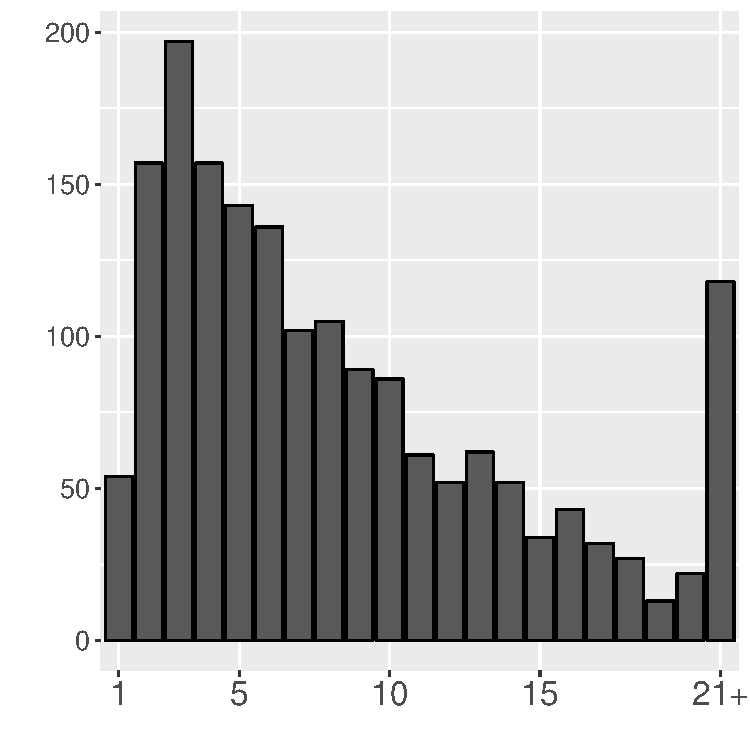
\includegraphics[width=0.7\textwidth]{figure/DEPositionAll.pdf}
	\caption{Order of all elements}
	\label{DEPositionAllF}
%	\end{center}
%\end{minipage}
\end{figure}
\begin{figure}
%\begin{minipage}{0.5\textwidth}
%	\begin{center}
	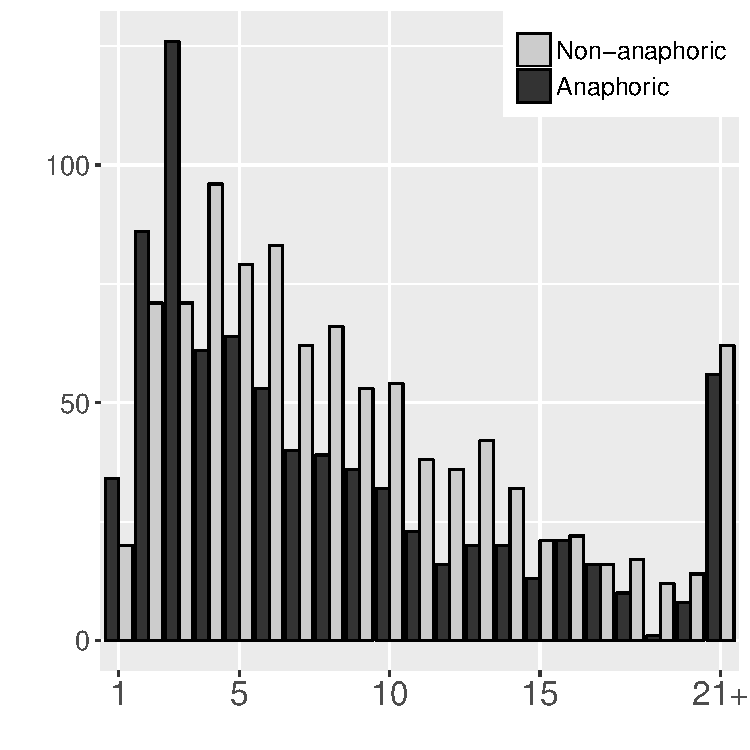
\includegraphics[width=0.7\textwidth]{figure/DEPositionIS.pdf}
	\caption{Word order vs.\ infoStatus}
	\label{DEPositionISF}
%	\end{center}
%\end{minipage}
\end{figure}
\begin{figure}
%\begin{minipage}{0.5\textwidth}
%	\begin{center}
	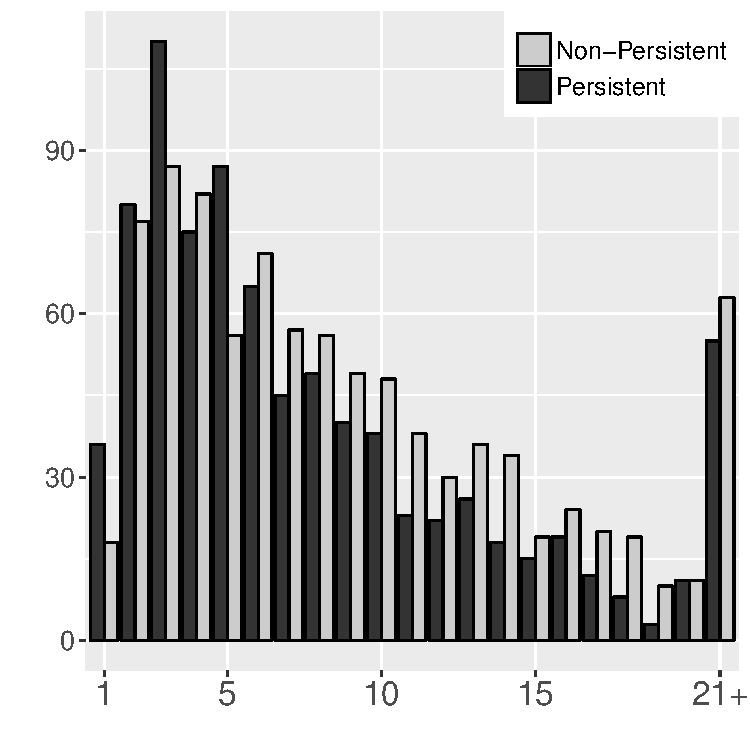
\includegraphics[width=0.7\textwidth]{figure/DEPositionPer.pdf}
	\caption{Word order vs.\ persistence}
	\label{DEPositionPerF}
%	\end{center}
%\end{minipage}
\end{figure}

Figure \ref{DiffAllF} shows the overall distribution of elements in terms of their distance from the predicate;
%\code{0} indicates that the element in question is the predicate itself,
\code{1} indicates that the element appears right before the predicate,
\code{2} indicates that there is one element between the preceding element and the following predicate, and so on.
If the element appears right after the predicate,
the distance is counted as \code{-1}.
Since the numbers of post-predicate elements are too small to achieve any generalization,
they are excluded from the figures.
Post-predicate elements will be discussed in comparison with dialogues
in \S \ref{WOPostPreEles}.

Figures \ref{DiffInfoStatusF} and \ref{DiffPerF} show the distance between the element and the predicate
depending on information status and persistence.
\chd{A linear mixed effects model of information status (the distance from the predicate and particles as fixed effects and the speaker as a random effect) indicates that
whereas the model with particles is significantly different from the model without them (likelihood ratio test, $p<0.001$),
the difference between the models with and without the distance from the predicate is only marginally significant ($p=0.060$).
This entails that the effect of particles significantly contributes to the model,
but the effect of the distance is inconclusive (see \ref{WOPrePredEles} for discussion).
On the other hand, a linear mixed effects model of persistence (fixed and random effects are the same above) shows that the effects of both particles and the distance are significant to the model ($p<0.01$ for both the model without particle and that without the distance).}
The results are also to be discussed more in \S \ref{WOPrePredEles}.


\begin{figure}
%\begin{minipage}{0.5\textwidth}
%	\begin{center}
	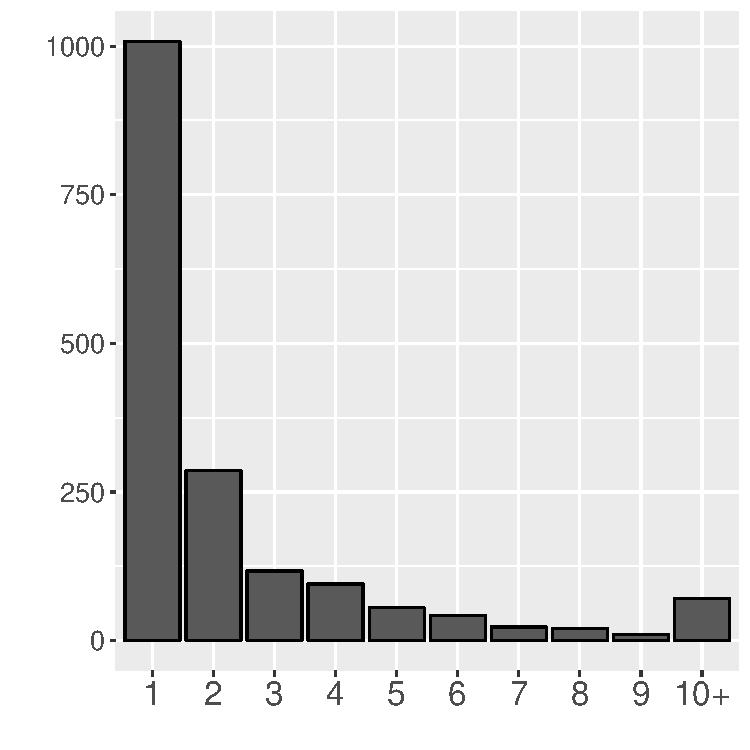
\includegraphics[width=0.7\textwidth]{figure/DiffAll.pdf}
	\caption{Distance from predicate}
	\label{DiffAllF}
%	\end{center}
%\end{minipage}
\end{figure}
\begin{figure}
%\begin{minipage}{0.5\textwidth}
%	\begin{center}
	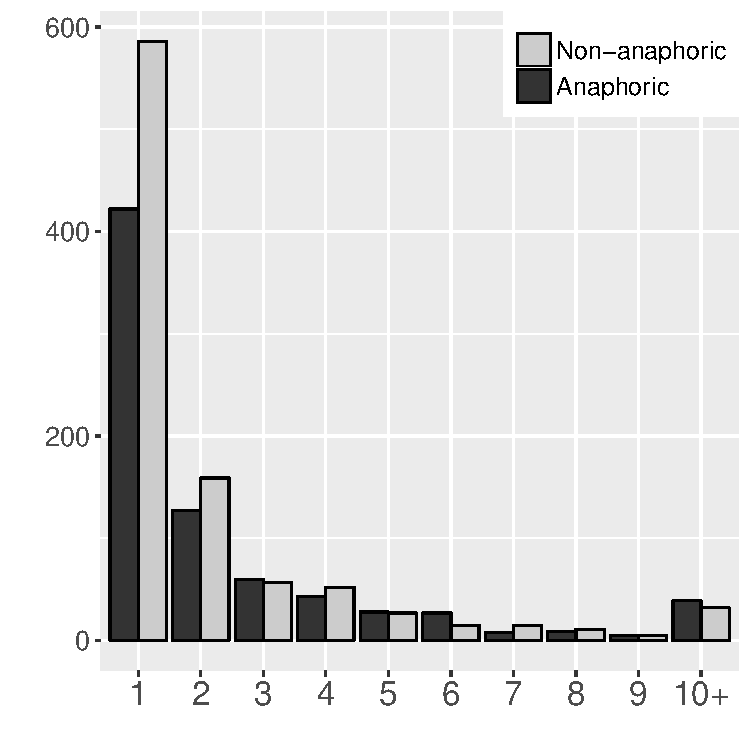
\includegraphics[width=0.7\textwidth]{figure/DiffInfoStatus.pdf}
	\caption{Distance from predicate vs.\ Information status}
	\label{DiffInfoStatusF}
%	\end{center}
%\end{minipage}
\end{figure}
\begin{figure}
%\begin{minipage}{0.5\textwidth}
%	\begin{center}
	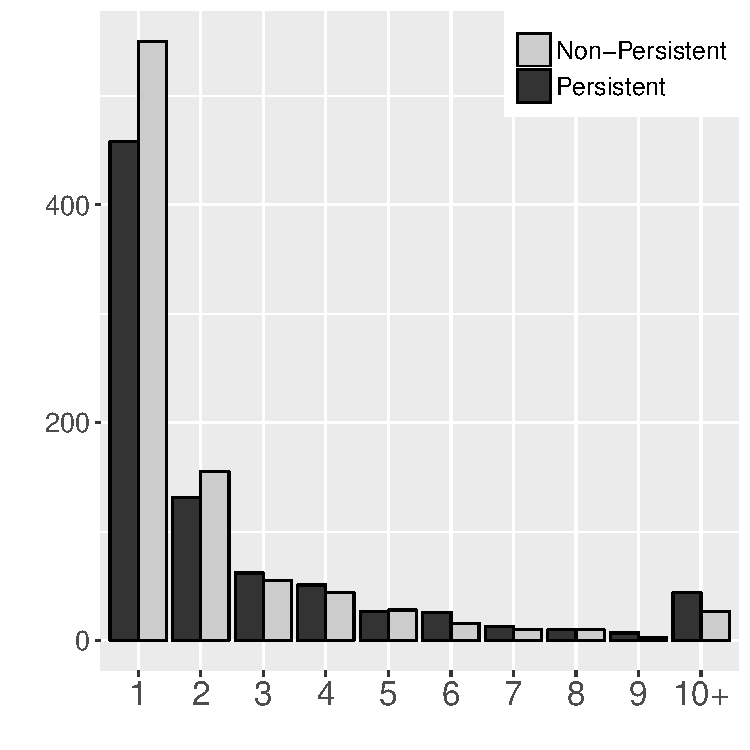
\includegraphics[width=0.7\textwidth]{figure/DiffPersistence.pdf}
	\caption{Distance from predicate vs.\ persistence}
	\label{DiffPerF}
%	\end{center}
%\end{minipage}
\end{figure}

%%----------------------------------------------------
%%----------------------------------------------------
\section{Clause-initial elements}\label{WOSentInitEles}

This section discusses clause-initial elements.
It will be argued that shared elements (i.e., unused, declining, inferable, or evoked elements) tend to appear clause-initially
in \S \ref{GivenAppearClause-Initially},
and that
persistent elements tend to appear clause-initially
in \S \ref{PersistentAppearClause-Initially}.
From these observations,
it will be generalized that topics tend to appear clause-initially,
as predicted from the previous literature.
Finally in \S \ref{TopicAppearClause-Initially},
I discuss the motivations for topics to appear clause-initially.


%%----------------------------------------------------
\subsection{Shared elements tend to appear clause-initially}\label{GivenAppearClause-Initially}

%\begin{figure}
%\begin{minipage}{0.5\textwidth}
%	\begin{center}
%	\includegraphics[width=0.95\textwidth]{figure/WO.pdf}
%	\caption{Word order within a clause}
%	\label{WOF}
%	\end{center}
%\end{minipage}
%\begin{minipage}{0.5\textwidth}
%	\begin{center}
%	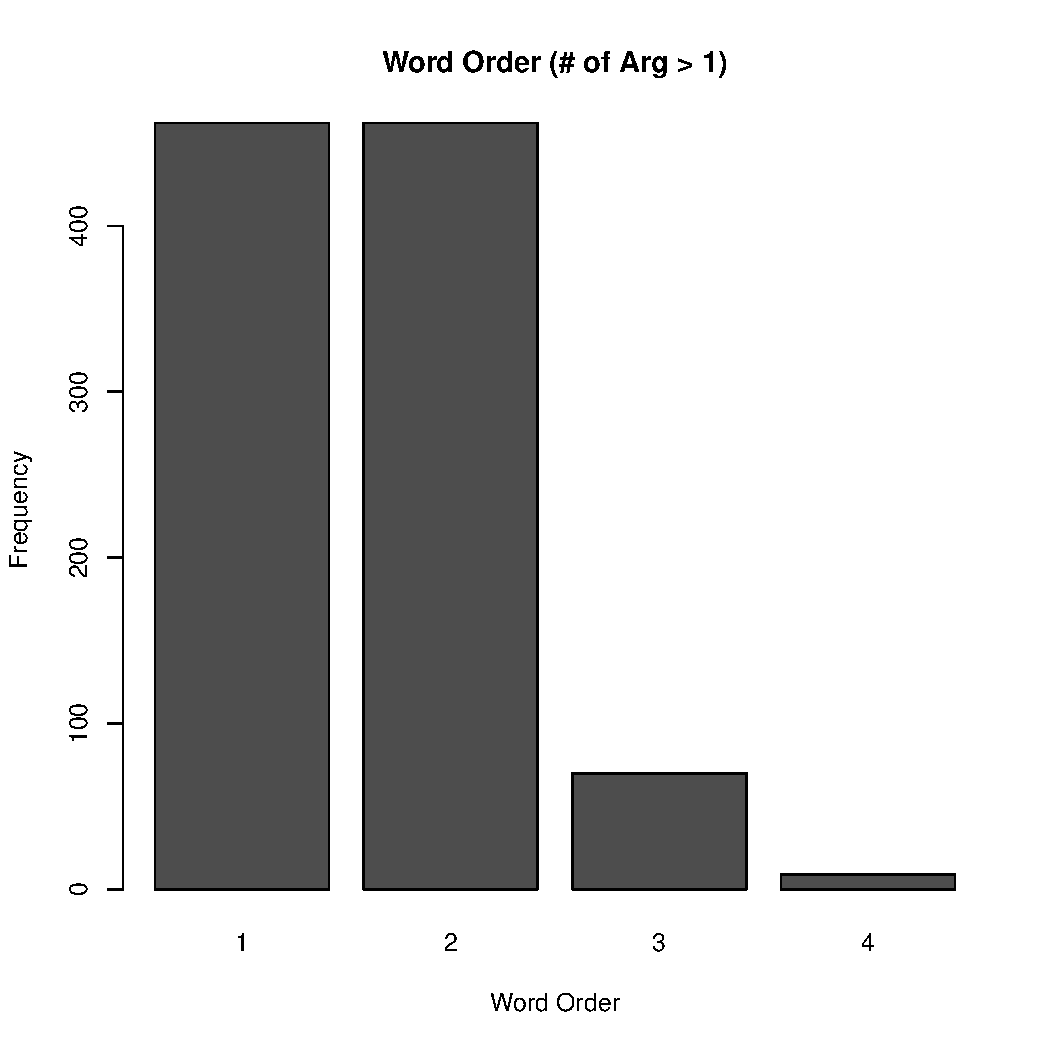
\includegraphics[width=0.95\textwidth]{figure/WO2.pdf}
%	\caption{Word order within a clause (\# of argument $>$ 1)}
%	\label{WO2F}
%	\end{center}
%\end{minipage}

%\begin{minipage}{0.5\textwidth}
%	\begin{center}
%	\includegraphics[width=0.95\textwidth]{figure/WOISGiven.pdf}
%	\caption{Word order vs.\ ASP (given, \# of argument $>$ 1)}
%	\label{WOISGivenF}
%	\end{center}
%\end{minipage}
%\begin{minipage}{0.5\textwidth}
%	\begin{center}
%	\includegraphics[width=0.95\textwidth]{figure/WOISNew.pdf}
%	\caption{Word order vs.\ ASP (new, \# of argument $>$ 1)}
%	\label{WOISNewF}
%	\end{center}
%\end{minipage}
%\end{figure}


Figure \ref{DEPositionISF} shows the frequency of elements and their positions
based on the information status.
Anaphoric elements appear most frequently in the third position.
On the other hand, the non-anaphoric elements appear most frequently in the fourth position,
but those in the fifth and sixth positions also appear frequently.
%This generalization still holds with another criterion.
%Figure \ref{WOF} shows the position of arguments within a clause (the arguments sharing the same predicate
%%considering only arguments of predicates
%potentially coded by \ci{ga} `\ab{nom}', \ci{o} `\ab{acc}', \ci{ni} `\ab{loc}'%
%	\footnote{
%	In Japanese, the same form \ci{ni} represent both locative and dative.
%	Here I simply included all \ci{ni}-coded elements as arguments.
%	}%
%).
%whereas Figure \ref{WOF} shows the overall orders of arguments.
%In Figure \ref{WOISF},
%clauses where more than one argument appears are considered.
%Figure \ref{WOISGivenF} shows the position of given arguments within a clause, considering only clauses where more than or equal to two arguments appear.
%Figure \ref{WOISNewF} shows the position of new arguments within a clause.
%As shown more clearly in these figures,
%given elements most frequently appear in the initial position,
%while new elements most frequently appear in the second position
%although those in the initial position are still frequent.
These distributions of elements in different information statuses appear to replicate the classic observation that
topics tend to appear earlier in a clause,
i.e., the from-old-to-new principle \cite{mathesius28,firbas64,danes70,kuno78,gundel88}
This is explicitly stated in \Next.
%
\ex. \label{oldnewprinciple}\tl{From-old-to-new principle}:
 In languages in which word order is relatively free,
 the unmarked word order of constituents is old,
 predictable information first and new, unpredictable information last.
 \hfill{(\citeA[][p.~54]{kuno78}, \citeA[][p.\ 326]{kuno04})}


This principle is motivated by accumulative nature of processing utterance;
old (or given) elements work as anchor that relates
the previous utterance and the following utterance.
%This does not indicate that all topics appear sentence initially.
%First,
%some kind of topic appear after the predicate rather than at the beginning as will be argued in \S \ref{WORdis},
%where
%the conditions of topics that appear sentence initially and post-predicatively will be discussed.
%Second,
%given foci can also appear at the beginning.
%As shown in \Next, for example,
This principle appears to be supported by examples such as the following.
%\ci{keeki-o} `cake-\ab{acc}' in line (ii),
%which refers to cake and ice cream in line (i),
%can be repeated after \ci{hee}
%and be treated as news.
%\ci{Keeki-o} `keeki-\ab{acc}' can also appear naturally before the predicate as shown in (ii)$^{\prime}$.
%%
%\ex. \a. \ag. koko-ni keeki-to aisu-ga oi-te at-ta-n-da-kedo \\
%		here-\ab{loc} cake-and ice.cream-\ab{nom} put-and exist-\ab{past}-\ab{nmlz}-\ab{cop}-though \\
%		`There were a piece of cake and ice cream,'
%	\bg. \EM{keeki-o} hanako-ga tabe-tyat-ta mitai \\
%		cake-\ab{acc} Hanako-\ab{nom} eat-\ab{pfv}-\ab{past} apparently \\
%		`but Hanako ate the cake.'
%	\bg.[(ii)$^{\prime}$] hanako-ga \EM{keeki-o} tabe-tyat-ta mitai \\
%		Hanako-\ab{nom} cake-\ab{acc} eat-\ab{pfv}-\ab{past} apparently \\
%		`but Hanako ate the cake.'
% \z.
% \b. hee, \{\EM{keeki-o} / Hanako-ga\}
%
In \Next,
\ci{sore} `it' in line c precedes,
which refers to \ci{kasi-pan} `sweet bread' back in line b,
the A element \ci{oziityan} `grandfather'.
%
\ex. \label{PronIni1}
% \ag. sarani uti-no sohu-tteiuno-ga okasi-ga sukina mono-de \\
%   moreover \ab{1}\ab{pl}-\ab{gen} 
% \a. In addition, my grandfather likes sweets,
 \ag. uti-no sohu-tteiuno-ga okasi-ga sukina mono-de \\
 		out-\ab{gen} grandfather-\ci{toiuno}-\ci{ga} sweet-\ci{ga} favorite thing-\ab{cop} \\
		`Our grandfather likes sweets.'
 \bg. yoku pan-ya-san-de \ul{\ul{kasi-pan}}-o kat-te kuru-n-desu-ga \\
   often bread-store-\ab{hon}-\ab{loc} sweet-bread-\ci{o} buy-and come-\ab{nmlz}-\ab{cop}.\ab{plt}-though \\
   `(He) often buys sweet bread and comes home,'
 \bg. e n \EM{sore-o} i maa yoowa \EMi{oziityan-wa} issyookenmee \fbox{taberu}-n-desu-keredomo \\
   \ab{fl} \ab{frg} that-\ci{o} \ab{frg} \ab{fl} in.a.word grandfather-\ci{wa} trying.best eat-\ab{nmlz}-\ab{cop}.\ab{plt}-though \\
   `that, he tries his best to eat it, but'
 \b. he cannot eat all and
 \b. gives leftovers to the dog...
  \hfill{(\code{S02M0198: 244.48-262.82})}
%S02M0198|00244484L|244.484271|252.337563|L|更に(0.433)うちの(0.569)祖父っていうのが(0.6)お菓子が好きなもの(0.204)で(0.39)よくパン屋さんで菓子パンを買ってくるんですが|/並列節ガ/|
%S02M0198|00253226L|253.226374|254.606404|L|買い過ぎてしまいまして|/テ節/|
%S02M0198|00255210L|255.209674|272.289576|L|(F え)(F ん)(0.648)それを(D い)(0.147)(F まー)要はお爺ちゃんは一生懸命食べるんですけれども(0.412)余って(0.268)それを犬に(0.194)あげ(0.315)てしまうので(1.403)(F その)残飯で太り(0.447)菓子パンで太り(0.696)味は覚えてグルメになるという最悪の(0.322)育ち方をしてしまいまして|/テ節/|
%

Note that \ci{sore} `that' in line c is not coded by \ci{wa} but by \ci{o}.
This shows that clause-initial shared elements are not necessarily coded by topic markers,
although it is predicted that elements coded by topic markers would more likely to appear clause-initially than those coded by case markers (see the discussion in \S \ref{WO:ClauseInit:Ident:Topic}).

Similarly in \Next,
\ci{sore} `it' in line c refers back to \ci{buraunkan} `cathode ray tube'
and appear at the beginning of the clause,
preceding other elements.
%
\ex.\label{PronIni2}
 \ag. oo-gata-no-ne \\
   large-type-\ab{gen}-\ab{fp} \\
   `(It's) a larger type (of cathode ray tube).'
 \bg. yoku maa a hooru-toka-ni aru-yoona oo-gata-no ee \ul{\ul{buraunkan}}-nan-da-kedomo \\
   often \ab{fl} \ab{fl} hall-etc.-\ab{dat} exist-like large-tyle-\ab{gen} \ab{fl} cathode.ray.tube-\ab{nmlz}-\ab{cop}-though \\
   `(It's) a large type of cathode ray tube typically equipped in a large hall, and'
 \bg. \EM{sore-o}-ne koo \EMi{kotti-kara} \EMi{kotti-ni} \fbox{moti-ageru}-toiu-yoona \\
  that-\ci{o}-\ab{fp} this.way here-from here-from bring-rise-\ab{quot}-like \\
  `this (cathode ray tube), (people) brought it from here to there.'
  \b. some people were doing something like that.
   \hfill{(\code{S05M1236: 471.26-490.38})}

%S05M1236|00462313L|462.313166|477.177522|L|(F ま)ブラウン管て言ってもですね(0.24)(F あのー)小型のブラウン管ではなくて(0.732)(F えー)(0.728)プロジェクション(F えー)チューブっつって(0.377)大きい(0.107)大型のね(0.135)よく(F まー)(F あ)(0.387)ホールとかに(0.134)あるような大型の(1.01)(F えー)ブラウン管なんだけども|/並列節ケドモ/|
%S05M1236|00477852L|477.851579|490.382975|L|(D す)それをね(0.401)こう(0.348)こっちからこっちに持ち上げると(0.5)いうような(0.155)朝から(0.457)朝から(D い)(0.421)夕方までこう(0.383)こっちからこっちに移すと(0.621)いうような仕事をしてる(F うー)同期の人もいました|[文末]|

However,
this is not the whole story;
there are many counter-examples where non-anaphoric precedes anaphoric.
Table \ref{GNT} shows the number of cases
where anaphoric precedes non-anaphoric and non-anaphoric precedes anaphoric within the same clause.
There are 102 cases where anaphoric precedes non-anaphoric,
while there are 63 cases where non-anaphoric precedes anaphoric.
The cases where anaphoric precedes non-anaphoric only slightly outnumber the cases where non-anaphoric precedes anaphoric.
63 cases (39.4\%) is too large a number to believe that
they are mere exceptions of the principle \ref{oldnewprinciple}.

\begin{table}
\centering
	\caption{Order of anaphoric \& non-anaphoric elements}
\begin{tabular}{rr}
	\toprule
	Anaphoric $\to$ Non-anaphoric & Non-anaphoric $\to$ Anaphoric \\
	\hline
	102 & 63 \\
	\bottomrule
\end{tabular}
	\label{GNT}
\end{table}

I do not claim that the principle \ref{oldnewprinciple} is not correct,
but I do claim that the principle does not apply to all cases.
Anaphoric elements precede non-anaphoric elements
if the anaphoric elements are assumed to refer to the ``same'' entity which has been already mentioned.
In other words,
shared elements precede non-anaphoric elements.
%I argue that identifiability is also one of the features of topichood.
%What I mean by ``topical'' is that an element has features that correlate with topic according to (\ref{ISFeatures}) in Chapter \ref{Framework}.
%In this case,
%being definite is a correlating feature with topic and definite elements are called ``topical''.
For example, in \Next,
\ci{mizu} `water' is repeatedly mentioned in the utterance,
but it is never produced clause-initially.
I argue that this is because
\ci{mizu} `water' in \Next[b] and later is not assumed to refer to the ``same'' entity already mentioned in the previous discourse.
%
\ex.\label{WO:ClauseInit:Given:mizu}
 \ag. desukara daitai iti-niti-ni ni-rittoru-no \EM{mizu-o} \ul{tot}-te kudasai-to iw-are-te \\
 so approximately one-day-for two-litter-\ab{gen} water-\ci{o} drink-and please-\ab{quot} tell-\ab{pass}-and \\
 `So we were told to drink two litters of water per day,'
 \bg. syokuzi-no toki-wa kanarazu magukappu-de ni-hai-bun-no \EM{mizu-o} \ul{nomi}-masu-si \\
 	meal-\ab{gen} time-\ci{wa} surely mug-with two-cup-amount-\ab{gen} water-\ci{o} drink-\ab{plt}-and \\
	`whenever we have meal, we drink two cups of water,'
 \bg. totyuu totyuu-de-mo kanarazu \EM{mizu-o} ho anoo \ul{nomi}-taku-naku-temo \\
 		on.the.way on.the.way-\ab{loc}-also surely water-\ci{o} \ab{frg} \ab{fl} drink-want-\ab{neg}-even.if \\
		`also on the way, even if we didn't want to drink water,'
 \bg. nom-as-areru-to iu kanzi-de \\
 	drink-\ab{caus}-\ab{pass}-\ab{quot} say feeling-\ab{cop} \\
	`we were forced to drink (water).'
 \b. they think that drinking water is very important.
  \hfill{(\code{S01F0151: 339.78-366.29})}
%S01F0151|00339776L|339.775512|341.443878|L|でこのティータイムなんですけれども|/並列節ケレドモ/|
%S01F0151|00341699L|341.698978|349.557717|L|この(0.43)標高の高いところでは(0.141)高山病という非常に危険な(0.329)可能性があるので(0.243)(F えー)水が非常に重要になります|[文末]|
%S01F0151|00349955L|349.954875|366.290044|L|ですから大体一日に二リットルの水を取ってくださいと言われて(0.316)食事の時は必ずマグカップで二杯分の水を(0.145)飲みますし(0.285)途中途中でも必ず水を(0.113)(D ほ)(0.114)(F あのー)(0.432)飲みたくなくても飲まされるという感じで(0.403)水分補給(0.297)を(0.632)重視しておりました|[文末]|


In the same way,
\ci{tenkan} `epilepsy' appears many times in \Next,
but never appear clause-initially.
%
\ex.\label{WO:ClauseInit:Given:tenkan}
 \ag. ato ik-kai \EM{tenkan} \EMi{okosi}-tara sinu-tte it-te-ta-n-desu-kedo \\
      moreover one-time.\ab{cl} epilepsy cause-\ab{cond} die-\ab{quot} say-\ab{past}-\ab{nmlz}-\ab{cop}.\ab{plt}-though \\
      `(The doctor) said that, if (my dog) get an epilepsy seizure once more, (the dog) would die, but...'
 \bg. mata so sookoo si-teru uti-ni \EM{tenkan} okosi-masi-te \\
      again \ab{frg} meanwhile do-\ab{prog} while-\ab{dat} epilepsy cause-\ab{plt}-and \\
      `meanwhile, (the dog) get an epilepsy seizure, and...'
 \b. The dog recovered this time, but got an epilepsy seizure several times and finally die. (130.8 sec omitted.)
 \bg. sono boku-ga dekakeru toki-ni moo noki-sita-de \EM{tenkan} \EMi{okosi}-te \\
      \ab{fl} \ab{1}\ab{sg}-\ci{ga} go.out when-\ab{dat} already eave-under-\ab{loc} epilepsy cause-and \\
      `When I leave (home), (the dog) had already gotten an epilepsy seizure, and...'
 \bg. tabun sin-dei-ta-n-da-roo-to \\
      probably die-\ab{prog}-\ab{past}-\ab{nmlz}-\ab{cop}-\ab{infr}-\ab{quot}\\
      `probably died...'
 \bg. ta noki-sita-de \EM{tenkan} \EMi{okosi}-ta-ga tame-ni \\
      \ab{frg} eave-under-\ab{loc} epilepsy cause-\ab{past}-\ab{gen} reason-\ab{dat} \\
      `just because (the dog) get an epilepsy seizure under the eaves...'
 \b. the dog could not get out of there and died, we [the family members] were talking like that.
 \src{S02M0198: 558.7-712.8}
%  \ex [飼い犬が]あと一回\EM{てんかん}起こしたら死ぬって言ってたんですけど
%  \ex またそそうこうしてるうちに\EM{てんかん}起こしまして
%  \ex ... (130.8秒省略。このときは復活したがその後数回てんかんを繰り返し、死んでしまう。)
%  \ex \label{ExTenkan3} その僕が出掛ける時にもう軒下で\EM{てんかん}起こして
%  \ex 多分死んでいたんだろうと
%  \ex \label{ExTenkan4} (た)軒下で\EM{てんかん}起こしたが為に
%  \ex その要は出られなくて
%  \ex 引っ掛かっちゃって
%  \ex 出られなくてそのまま死んじゃったんじゃないのっていう話をしたんですけど\\
%\src{S02M0198: 558.7-712.8}


Whether the speaker refers to the shared entity mentioned previously
depends on the speaker's subjective judgement rather than objective reasoning.
In \Next, for example,
the anaphoric element \ci{kuruma} `car' in line c does not appear clause-initially for the same reason as \LLast and \Last.
However, \ci{kuruma} `car' in line b and d are clearly the same entity.
%
\ex.\label{WO:ClauseInit:Given:kuruma}
 \ag. kirauea-kazan-mo mappu-o kai-masi-te \\
 		Kilauea-volcano-also map-\ci{o} buy-\ab{plt}-and \\
		`Also for Kilauea, (we) bought a map and'
 \bg. de zibun-tati-de ma rentakaa \EM{kuruma-o} \ul{tobasi}-te e iki-masi-ta \\
 		then self-\ab{pl}-by \ab{fl} rent-a-car car-\ci{o} drive-and \ab{fl} go-\ab{plt}-\ab{past} \\
		`(we) drove there by rent-a-car by ourselves.'
 \b.[] (83.52 sec talking about the mountain.)
 \bg. de anoo jibun-no koko koko-de tyotto tome-te miyoo-to omot-ta toko-ni koo \EM{kuruma-o} \ul{tome}-te \\
 		and \ab{fl} self-\ab{gen} \ab{frg} here-\ab{loc} a.bit stop-and try-\ab{quot} think-\ab{past} place-\ab{dat} this.way car-\ci{o} stop-and \\
	 	`At the place (we) wanted to stop, (we) stopped the car,'
 \b. you can take pictures and so on.
 \hfill{(\code{S00F0014: 843.23-940.34})}
%
%S00F0014|00843233L|843.23315|850.162512|L|(F あのー)キラウエア火山もマップを買いましてで自分達で(0.363)(F ま)レンタカー(0.102)車を(0.376)飛ばして(0.367)(F え)行きました|[文末]|
% ...
%S00F0014|00933685L|933.684509|940.33856|L|で(0.299)(F あのー)自分のここここでちょっと止めてみようと思ったとこにこう車を止めて(0.398)(F まー)その写真を撮ったり|<タリ節>|大きい切れ目−係り先なし

I argue that, in this case, the speaker does not care about the identity of the car.
Rather, she focuses on talking about her trip to Kirauea;
the car she was in is not important for this speech.
As will be discussed in \S \ref{PersistentAppearClause-Initially},
importance as well as the identity of the entity contributes to word order in spoken Japanese.
Important (i.e., persistent) elements appear clause-initially.

Interestingly,
these elements which are repeatedly mentioned but never appear clause-initially are not mentioned by zero or overt pronouns.
It is especially difficult to zero-pronominalize \ci{tenkan} `epilepsy' in \LLast[b-f] and \ci{kuruma} `car' in \Last[d].%
 \footnote{
 It is difficult to apply this test in \ref{WO:ClauseInit:Given:mizu} because \ci{mizu} `water' accompanies numeral modifiers such as 
 `of two litters' and `two cup of'.
 }
Zero pronouns are considered to be the most accessible topics \cite[17]{givon83}.
To zero-pronominalize,
the speaker needs to provide signals to let the hearer know which is the topic as will be discussed in \ref{TopicAppearClause-Initially}.

%%
%\ex.
% \ag. koko-ni kuri-gohan-to yaki-zakana-ga oi-te at-ta-kara minna-de tabe-yoo-to omot-ta-n-da-kedo \\
% 		here-\ab{loc} chestnut-rice-and baked-fish-\ab{nom} put-and exist-because all-by eat-will-\ab{quot} think-\ab{past}-\ab{nmlz}-\ab{cop}-though \\
%		`Here there had been chestnut rice and baked fish and I wanted to eat them with everybody, but'
% \bg. \EM{gohan-\{o/wa/{\O}\}} hanako-ga tabe-tyat-ta-n-da-tte \\
% 		rice-\{\ab{acc}/\ci{wa}/{\O}\} Hanako-\ab{nom} eat-\ab{pfv}-\ab{past}-\ab{nmlz}-\ab{cop}-\ab{rep} \\
%		`Hanako ate the rice (and the rice is gone).'
% \bg.[b$^{\prime}$.] hanako-ga \EM{gohan-\{?o/??wa/{\O}\}} tabe-tyat-ta-n-da-tte \\
% 		Hanako-\ab{nom} rice-\{\ab{acc}/\ci{wa}/{\O}\} eat-\ab{pfv}-\ab{past}-\ab{nmlz}-\ab{cop}-\ab{rep} \\
%		`Hanako had eaten meal (so we cannot eat together).'
%%%% イントネーションも重要。b'で「ごはん」に強勢があると、indefiniteとしか解釈されない。
%
%Although the judgement is subtle,
%in \Last[b], where \ci{gohan} `rice' precedes the agent `Hanako',
%\ci{goahn} `rice' inclines to be interpreted as \ci{kuri-gohan} `chestnut rice' which has appeared in the previous line a.
%On the other hand,
%in \Last[b$^{\prime}$], where \ci{gohan} `rice' is preceded by the agent `Hanako',
%\ci{gohan} `rice' inclines to be interpreted as meal in general.%
%	\footnote{
%	In Japanese, \ci{gohan} `rice' is ambiguous between rice and meal in general.
%	}
%Moreover,
%\ci{o}-, \ci{wa}- and zero-codings are possible in \Last[b],
%whereas only zero-coding is natural in \Last[b$^{\prime}$].
%In \Last, \ci{o}-coding is possible because it is separated from the predicate.
%In spoken Japanese,
%P elements tend to be overtly coded if they are separated from the predicate \cite{fry01}.
%\ci{Wa}-coding is possible because \ci{gohan} `rice' appeared in the previous discourse.
%I believe the zero particle in this case is {\O$_{t}$},
%which is felicitous regardless of the activation status of the referent of \ci{gohan} `rice'.
%The information structure of \Last[a] can be represented as \Next.
%%
%\ex.
%% \ag. [gohan-o hanako-ga tabe-tyat-ta]$_{F}$ \\
%%			rice-\ab{acc} Hanako-\ab{nom} eat-\ab{pfv}-\ab{past} \\
%	\ag.  [gohan-\{o/wa/{\O}\}]$_{T}$ [hanako-ga tabe-tyat-ta]$_{F}$ \\
%			rice-\{\ab{acc}/\ci{wa}/{\O}\} Hanako-\ab{nom} eat-\ab{pfv}-\ab{past} \\
%
%I argue that \ci{o}-coded \ci{gohan} `rice' in the initial position is still topic to some extent,
%although it is not coded by the topic marker \ci{wa};
%P in the initial position, preceding focus A,
%only refers to elements which has been activated in the hearer's mind.
%\LLast[b] cannot receive the interpretation \LLast[b$^{\prime}$].
%If this position is for focus, there should be no such constraint;
%focus is by default non-anaphoric and has not been activated in the hearer's mind.
%Moreover, most given Ps are still coded by \ci{o} `\ab{acc}' as will be discussed below.
%
%In \LLast[b$^{\prime}$], on the other hand,
%\ci{gohan} `rice' cannot be coded by \ci{o} or \ci{wa}.
%Assuming that the information structure of \Last[b] is \Next,
%\ci{gohan} is felicitously coded by \ci{o} `\ab{acc}' because
%non-contrastive focus P elements cannot felicitously coded by \ci{o}.
%\exg. [hanako-ga gohan-{\O} tabe-tyat-ta]$_{F}$ \\
%		Hanako-\ab{nom} rice-{\O} eat-\ab{pfv}-\ab{past} \\
%
%I claim \ci{wa}-coding is impossible because
%of the incompatible characteristics of \ci{wa}-coding and the element's position;
%\ci{wa} codes activated element at issue and the element between the focus agent and the focus predicate is also interpreted as focus.
%Since focus elements are tend to be indefinite and non-anaphoric,
%\ci{gohan} `rice' in \LLast[b$^{\prime}$] inclines to be interpreted as indefinite and new.
%Still, I claim that \ci{gohan-o} `rice-\ab{acc}' in \LLast[b] is focus but given
%because it appears in the initial position preceding other focus elements.

%This claim seems difficult to test in the corpus because
%there is no definite markers in Japanese.
From the discussion above,
there are at least two predictions testable in the corpus.
Firstly, since evoked and inferable elements are coded by topic markers as shown in Chapter \ref{Particles},
it is predicted that
elements coded by topic markers tend to appear earlier in a clause (\S \ref{WO:ClauseInit:Ident:Topic}).
This is because elements assumed by the speaker to be evoked or inferable
are also assumed to be shared.
Secondly,
since pronouns essentially code shared elements which have been mentioned,
pronouns are also predicted to appear earlier in a clause (\S \ref{WO:ClauseInit:Ident:Pron}).
Both predictions are confirmed in the following investigations.
Thirdly, I will show that clause-initial elements are not sensitive to activation cost;
unused elements can also appear clause-initially (\S \ref{WO:ClauseInit:Ident:ActStatus}).
Evoked, inferable, declining, and unused elements are shared
(See Table \ref{ActStatusCorpus}).
Therefore, the claim that shared elements appear clause-initial is supported.

%%----------------------------------------------------
\subsubsection{Topic-coded elements appear clause-initially}\label{WO:ClauseInit:Ident:Topic}

\begin{figure}
%\begin{minipage}{0.5\textwidth}
	\begin{center}
	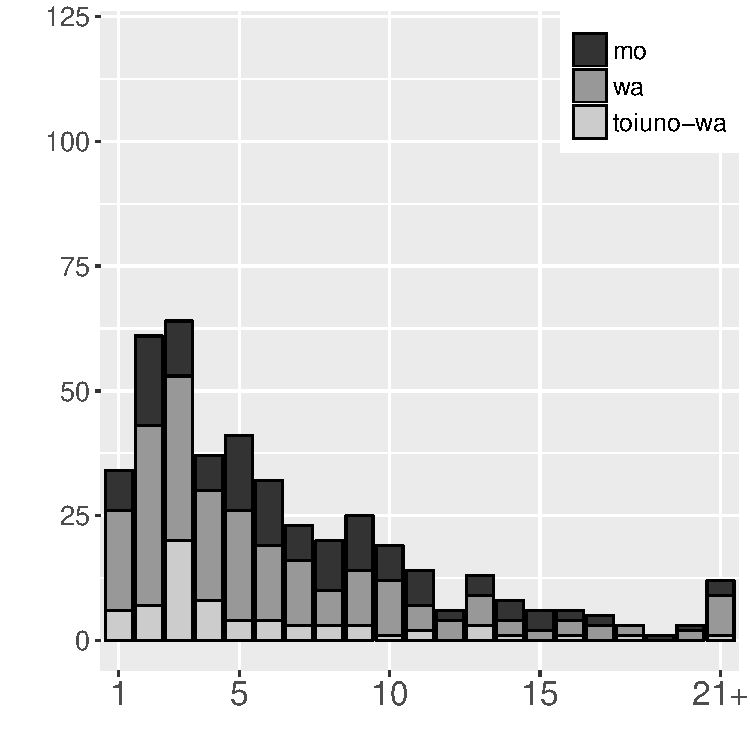
\includegraphics[width=0.7\textwidth]{figure/WOTopPar.pdf}
	\caption{Order of arguments coded by topic markers}
	\label{WOTopParF}
	\end{center}
%\end{minipage}
\end{figure}
\begin{figure}
%\begin{minipage}{0.5\textwidth}
	\begin{center}
	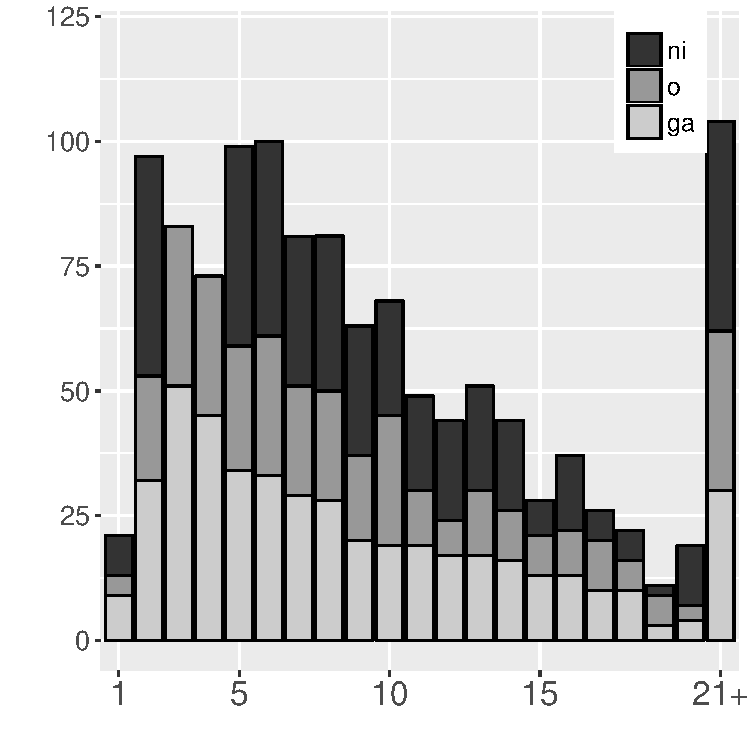
\includegraphics[width=0.7\textwidth]{figure/WOCasePar.pdf}
	\caption{Order of arguments coded by case markers}
	\label{WOCaseParF}
	\end{center}
%\end{minipage}
\end{figure}

%%% \ref{Par:ArgStr}で一部議論重複
Let us test the prediction that elements coded by topic markers tend to appear earlier in a clause.
Figure \ref{WOTopParF} shows the distribution of topic-coded elements
and their positions.
Compare this figure with Figure \ref{WOCaseParF},
which shows the distribution of case-coded elements and their positions.
It is clear that
elements coded by topic markers are more skewed to earlier positions within a clause as compared with those coded by case markers.

\Next is an example of \ci{wa}-coded element appearing clause-initially.
The \ci{wa}-coded element \ci{hone} `bone' in line a,
which has been discussed in the previous discourse,
is intervened with the locative (a tomb for animals in the temple).
The intervening part is long and the predicate finally appears in line d.
%
\ex.
	\ag. ee suriipii-no itibu-no oo \EM{hone-wa} \\
		\ab{fl} Sleepy-\ab{gen} part-\ab{gen} \ab{fl} bone-\ci{wa} \\
		`Part of bone of Sleepy (dog's name),'
	\bg. sono morimati-no watasi-no senzo-no o hait-teru otera-no \\
		that Morimachi-\ab{gen} \ab{1}\ab{sg}-\ab{gen} ancestor-\ci{gen} \ab{fl} enter-\ab{prog} temple-\ab{gen} \\
		`the temple in Morimachi where my ancestors were there,'
	\bg. yahari ano doobutu-no kuyootoo-ga ari-masu \\
		again that animal-\ab{gen} tomb-\ci{ga} exist-\ab{plt} \\
		`there're tombs for animals,'
	\bg. sotira-no hoo-ni \ul{osame}-masite-ne \\
		that-\ab{gen} direction-\ab{dat} place-\ab{plt}-and \\
		`(we) placed (his bone) there.'
	\hfill{(\code{S02M1698: 620.12-634.26})}
%S02M1698|00620119L|620.118778|634.26275|L|(F えー)スリーピーの一部の(0.379)(F おー)骨は(0.438)その<FV>森町の(0.669)私の先祖の(0.598)(F お)入ってるお寺の(0.465)やはり(F あの)動物の供養塔があります(0.358)そちらの方に納め(0.347)ましてね|/テ節/|

In \Next,
\ci{sono ko} `that puppy',
whose referent has appeared in the previous line a,
is also an example of \ci{wa}-coded element appearing clause-initially.
The element is also intervened by another argument `distemper'.
%
\ex.
	\ag. mosi \ul{\ul{koinu-o}} kat-tesimat-tara \\
		if puppy-\ci{o} keep-\ab{pfv}-\ab{cond} \\
		`If you decided to keep a new puppy,'
	\bg. \EM{sono} \EM{ko-wa} mata zisutenpaa-ni \ul{kakat}-te sin-zyau-kara \\
			that puppy-\ci{wa} again distemper-\ab{dat} catch-and die-\ab{pfv}-because \\
			`the puppy will die of distemper again, so'
	\b. keep a new puppy after this winter, this is what we were told by the vet.
	\hfill{(\code{S02M0198: 108.68-126.70})}
%
%S02M0198|00108681L|108.680591|126.700531|L|冬を越さないと(0.407)ジステンパーの細菌が(0.47)庭にいるままで死んでくれないから(0.431)もし小犬を飼っ(0.843)てしまったら(0.382)その子はまたジステンパーに掛かって死んじゃうから(0.584)冬を越してから(0.403)新しい犬を飼ってくれ(0.356)と僕らは言われていたもので|<並列節デ>|大きい切れ目−係り先なし

%\Next is an example of given elements that are neither coded by topic markers nor put in clause-initially.
%The element \ci{mizu} `water' appears three times in \Next,
%all of which are given.
%\ex.\label{WO:Ex:mizu}
% \ag. desukara daitai iti-niti-ni ni-rittoru-no \EM{mizu-o} \ul{tot}-te kudasai-to iw-are-te \\
% so approximately one-day-for two-litter-\ab{gen} water-\ab{acc} drink-and please-\ab{quot} tell-\ab{pass}-and \\
% `So we were told to drink two litters of water per day,'
% \bg. syokuzi-no toki-wa kanarazu magukappu-de ni-hai-bun-no \EM{mizu-o} \ul{nomi}-masu-si \\
% 	meal-\ab{gen} time-\ci{wa} surely mug-with two-cup-amount-\ab{gen} water-\ab{acc} drink-\ab{plt}-and \\
%	`whenever we have meal, we drink two cups of water,'
% \bg. totyuu totyuu-de-mo kanarazu \EM{mizu-o} ho anoo \ul{nomi}-taku-naku-temo \\
% 		on.the.way on.the.way-\ab{loc}-also surely water-\ab{acc} \ab{frg} \ab{fl} drink-want-\ab{neg}-even.if \\
%		`also on the way, even if we didn't want to drink water,'
% \bg. nom-as-areru-to iu kanzi-de \\
% 	drink-\ab{caus}-\ab{pass}-\ab{quot} say feeling-\ab{cop} \\
%	`we were forced to drink (water).'
% \b. they think that drinking water is very important.
%  \hfill{(\code{S01F0151: 339.78-366.29})}
%%S01F0151|00339776L|339.775512|341.443878|L|でこのティータイムなんですけれども|/並列節ケレドモ/|
%%S01F0151|00341699L|341.698978|349.557717|L|この(0.43)標高の高いところでは(0.141)高山病という非常に危険な(0.329)可能性があるので(0.243)(F えー)水が非常に重要になります|[文末]|
%%S01F0151|00349955L|349.954875|366.290044|L|ですから大体一日に二リットルの水を取ってくださいと言われて(0.316)食事の時は必ずマグカップで二杯分の水を(0.145)飲みますし(0.285)途中途中でも必ず水を(0.113)(D ほ)(0.114)(F あのー)(0.432)飲みたくなくても飲まされるという感じで(0.403)水分補給(0.297)を(0.632)重視しておりました|[文末]|

%I argue that `water' in \Last is interpreted as indefinite and the givenness of `water' does not matter in this narrative.
%This is because \ci{mizu} `water' appears non-initial position.
%Of course there are definite referents appearing non-initial position.
%However, the givenness of those referents are still not important.
%Consider the following example.
%%
%\ex.\label{WO:Ex:kuruma}
% \ag. kirauea-kazan-mo mappu-o kai-masi-te \\
% 		Kilauea-volcano-also map-\ab{acc} buy-\ab{plt}-and \\
%		`Also for Kilauea, (we) bought a map and'
% \bg. de zibun-tati-de ma rentakaa \EM{kuruma-o} \ul{tobasi}-te e iki-masi-ta \\
% 		then self-\ab{pl}-by \ab{fl} rent-a-car car-\ab{acc} drive-and \ab{fl} go-\ab{plt}-\ab{past} \\
%		`(we) drove there by rent-a-car by ourselves.'
% \b.[] (83.52 sec talking about the mountain.)
% \bg. de anoo jibun-no koko koko-de tyotto tome-te miyoo-to omot-ta toko-ni \\
% 		and \ab{fl} self-\ab{gen} \ab{frg} here-\ab{loc} a.bit stop-and try-\ab{quot} think-\ab{past} place-\ab{loc} \\
%	 	`At the place (we) wanted to stop,'
% \bg. koo \EM{kuruma-o} \ul{tome}-te \\
% 		this.way car-\ab{acc} stop-and \\
%		`(we) stopped the car,'
% \b. you can take pictures and so on.
% \hfill{(\code{S00F0014: 843.23-940.34})}
%%
%%S00F0014|00843233L|843.23315|850.162512|L|(F あのー)キラウエア火山もマップを買いましてで自分達で(0.363)(F ま)レンタカー(0.102)車を(0.376)飛ばして(0.367)(F え)行きました|[文末]|
%% ...
%%S00F0014|00933685L|933.684509|940.33856|L|で(0.299)(F あのー)自分のここここでちょっと止めてみようと思ったとこにこう車を止めて(0.398)(F まー)その写真を撮ったり|<タリ節>|大きい切れ目−係り先なし
%
%In \Last,
%\ci{kuruma} `car' is mentioned in lines b and d.
%Since it is reasonable to think that the speakers drove the same car while they were travelling,
%\ci{kuruma} `car' in line d is inferred as definite.
%However, the definiteness or givenness of the car here is irrelevant to the discourse;
%the speaker is talking about their travel to Kilauea not about the car.
%Therefore,
%\ci{kuruma} is coded by the case marker \ci{o} and appears non-initial position, i.e., immediately before the predicate as will be discussed in \S \ref{WOPrePredEles}.

\ci{Wa} appearing at the initial position is already conventionalized, and
it is possible to examine by acceptability judgements.
It is not acceptable for \ci{wa}-coded P to appear between the focus agent and the predicate except for contrastive reading of \ci{wa}.
%	\footnote{
%	Contrastive \ci{wa} appearing in this position will be
%	discussed more in detail in \S \ref{WODiscussion}.
%	}
As the contrast among \Next[a-c] shows,
the zero-coded P \ci{hon} `book' in \Next[a] right before the predicate is acceptable,
while the \ci{wa}-coded \ci{hon} `book' in the same position as in \Next[b] is not acceptable.
To express the idea of \Next[b],
the \ci{wa}-coded P should precede A \ci{taroo} `Taro'.
%
\ex. \ag. \ul{taroo-ga} \EM{hon} yon-deru-yo \\
		Taro-\ci{ga} book read-\ab{prog}-\ab{fp} \\
		`Taro is reading a book.'
	\bg. ??\ul{taroo-ga} \EM{hon-wa} yon-deru-yo \\
		Taro-\ci{ga} book-\ci{wa} read-\ab{prog}-\ab{fp} \\
		`Taro is reading the book.'
	\bg. \EM{hon-wa} \ul{taroo-ga} yon-deru-yo \\
		book-\ci{wa} Taro-\ci{ga} read-\ab{prog}-\ab{fp} \\
		`Taro is reading the book.'
		\hfill{(Constructed)}

There is only one example (out of 9 \ci{wa}-coded Ps) in the corpus
where \ci{wa}-coded P is preceded by \ci{ga}-coded A.
This \ci{wa}-coded P is contrastive, which will be discussed in \S \ref{WODiscussion}.

I propose the hypothesis that elements which belong to the same unit of information structure appear adjacent within a clause.
I call this information-structure continuity principle in word order.
%
\ex. \label{IScontinuityP}\tl{Information-structure continuity principle}:
 A unit of information structure is continuous in a clause;
 i.e., elements which belong to the same unit are adjacent with each other.

This principle explains why \LLast[b] is not acceptable,
while \LLast[a,c] are acceptable.
The information structure of each of the examples \LLast are represented in \Next.
In \Next[b],
the topic P element \ci{hon-wa} `book-\ci{wa}' intervenes two focus elements \ci{taroo-ga} `Taro-\ci{ga}' and \ci{yon-deru} `read-\ab{prog}', which is not acceptable.
In \Next[c], on the other hand,
the topic P does not intervene the domain of focus,
and the whole sentence is acceptable.
In \Next[a],
all the elements including \ci{hon} `book' belong to focus
and hence \ci{hon} in this position is acceptable.
%
\ex. \ag. [\ul{taroo-ga} \EM{hon} yon-deru]$_{F}$-yo \\
		Taro-\ci{ga} book read-\ab{prog}-\ab{fp} \\
		`Taro is reading a book.'
	\bg. ??[\ul{taroo-ga}]$_{F}$ [\EM{hon-wa}]$_{T}$ [yon-deru]$_{F}$-yo \\
		Taro-\ci{ga} book-\ci{wa} read-\ab{prog}-\ab{fp} \\
		`Taro is reading the book.'
	\bg. [\EM{hon-wa}]$_{T}$ [\ul{taroo-ga} yon-deru]$_{F}$-yo \\
		book-\ci{wa} Taro-\ci{ga} read-\ab{prog}-\ab{fp} \\
		`Taro is reading the book.'

Interestingly,
it is possible for \ci{wa}-coded A to be preceded by \ci{o}-coded P as shown in \Next[a] (compare this with \Next[b]).
%
\ex.
\ag. \ul{hon-o} \EM{taroo-wa}  yon-deru-yo \\
		book-\ci{o} Taro-\ci{wa} read-\ab{prog}-\ab{fp} \\
		`Taro is reading the book.'
\bg. \ul{hon-o} \EM{taroo-ga} yon-deru-yo \\
		book-\ci{o} Taro-\ci{ga} read-\ab{prog}-\ab{fp} \\
		`Taro is reading the book.'

As has been argued above,
the preposed P, \ci{hon-o} `book-\ci{o}' in \Last,
is topical, which is represented as in \Next.
%
\ex.
\ag. [\ul{hon-o} \EM{taroo-wa}]$_{T}$  [yon-deru]$_{F}$-yo \\
		book-\ci{o} Taro-\ci{wa} read-\ab{prog}-\ab{fp} \\
		`Taro is reading the book.'
\bg. [\ul{hon-o}]$_{T}$ [\EM{taroo-ga} yon-deru]$_{F}$-yo \\
		book-\ci{o} Taro-\ci{ga} read-\ab{prog}-\ab{fp} \\
		`Taro is reading the book.'

As shown in \Last[a],
the two topic elements \ci{hon-o} `book-\ci{o}' and \ci{taroo-wa} `Taro-\ci{wa}' are adjacent with each other and hence this sentence is acceptable.
Also in \Last[b],
the only topic element \ci{hon-o} `book-\ci{o}' does not intervene the focus elements \ci{taroo-ga}, which is predicted to be acceptable.
\ci{Hon-o} `book-\ci{o}' could be focus instead of topic in \LLast[b], since given elements can be focus.
But it is reasonable to think of a situation where given focus elements are preposed
for the sentence to be a smooth transition from the previous sentence.
The information-structure continuity principle \ref{IScontinuityP} still holds in either case.

Note that \ref{IScontinuityP} does not refer to word order;
rather, it is about adjacency.
I argue that this principle is also at work in intonation (see Chapter \ref{Intonation}).

What is the difference between clause-initial elements coded by topic markers and those coded by case markers?
As has been discussed in \S \ref{Par:ArgStr:TopHierarchy},
there is a hierarchy of topic coding \ref{ASPGivenSchema},
which is repeated here as \Next.
%
\ex.
 A, S $>$ P

The hierarchy indicates that
evoked or inferable A and S are more likely to be coded by topic markers than P in the same status.
Word order is not affected by this hierarchy.
Figure \ref{WOSGivenF} and \ref{WOPGivenF} show word order of
anaphoric S and P, respectively.
Compare these with Figure \ref{WOSNewF} and \ref{WOPNewF},
which show word order of non-anaphoric S and P.
Word order of A is omitted because the number is too small.
As can be seen from the contrasts between Figure \ref{WOSGivenF} and \ref{WOSNewF} and between Figure \ref{WOPGivenF} and \ref{WOPNewF},
anaphoric elements are more likely to appear earlier in a clause than non-anaphoric elements.
Although the contrast is less clear between anaphoric vs.~non-anaphoric P,
especially notable is that there are three times as much anaphoric Ps as non-anaphoric Ps in the third position.
(There are 27 anaphoric Ps in the third position,
while there are only 10 non-anaphoric P.)
I speculate that the contrast is less clear in anaphoric vs.~non-anaphoric P than S because there are cases like \ref{WO:ClauseInit:Given:mizu} and \ref{WO:ClauseInit:Given:tenkan},
where the element is annotated as anaphoric but is considered to be not shared;
in this case, P appear pre-predicatively rather than clause-initially.
Therefore, I argue that,
while elements coded by topic markers are likely to appear earlier in a clause,
word order is independent of topic marking.
Topic markers are sensitive to given-new taxonomy as has been discussed in Chapter \ref{Particles};
clause-initial position is sensitive to shared-ness.
Topic markers and word order are sensitive to different aspects of topichood.

\begin{figure}
%\begin{minipage}{0.5\textwidth}
	\begin{center}
	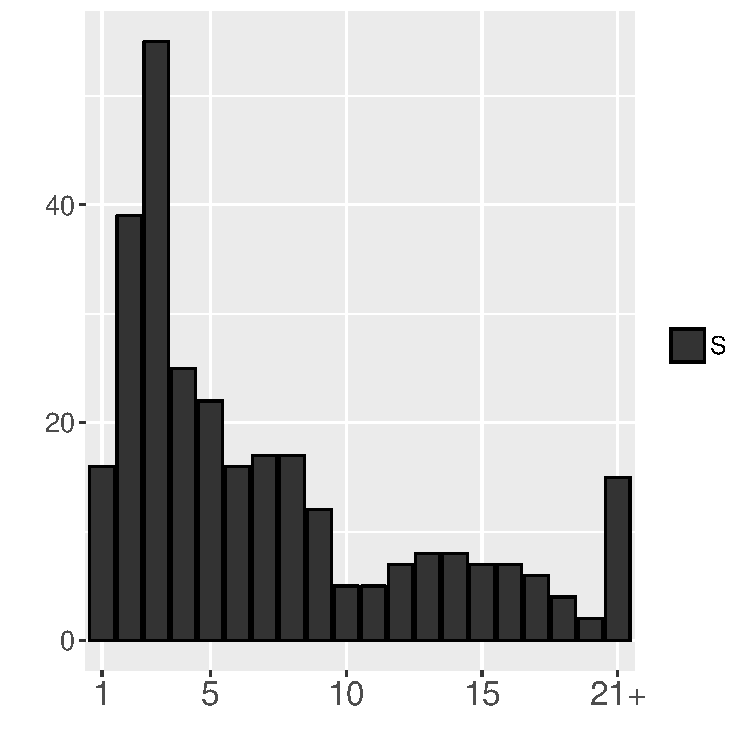
\includegraphics[width=0.6\textwidth]{figure/WOSGiven.pdf}
	\caption{Word order of anaphoric S}
	\label{WOSGivenF}
	\end{center}
%\end{minipage}
\end{figure}
\begin{figure}
%\begin{minipage}{0.5\textwidth}
	\begin{center}
	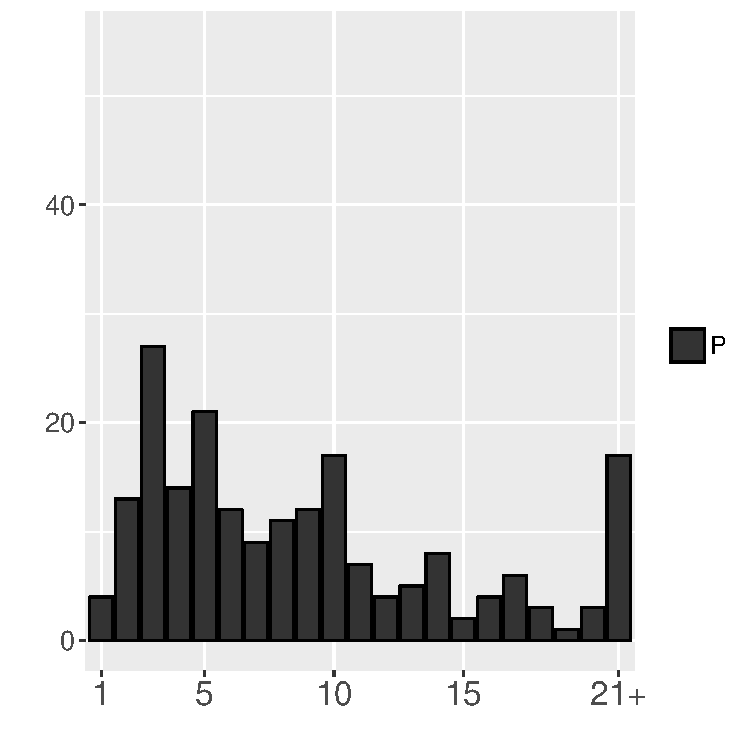
\includegraphics[width=0.6\textwidth]{figure/WOPGiven.pdf}
	\caption{Word order of anaphoric P}
	\label{WOPGivenF}
	\end{center}
%\end{minipage}
\end{figure}
\begin{figure}
%\begin{minipage}{0.5\textwidth}
	\begin{center}
	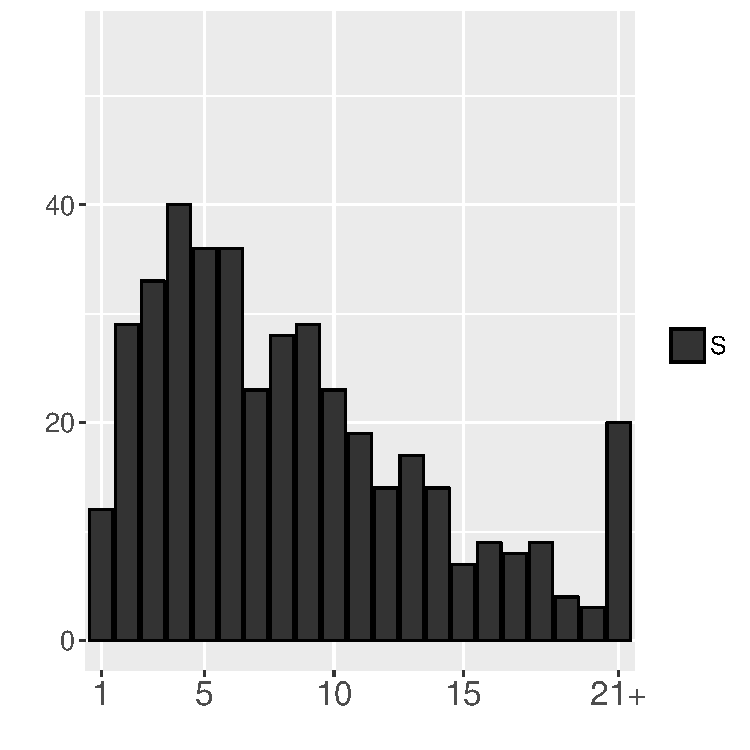
\includegraphics[width=0.6\textwidth]{figure/WOSNew.pdf}
	\caption{Word order of non-anaphoric S}
	\label{WOSNewF}
	\end{center}
%\end{minipage}
\end{figure}
\begin{figure}
%\begin{minipage}{0.5\textwidth}
	\begin{center}
	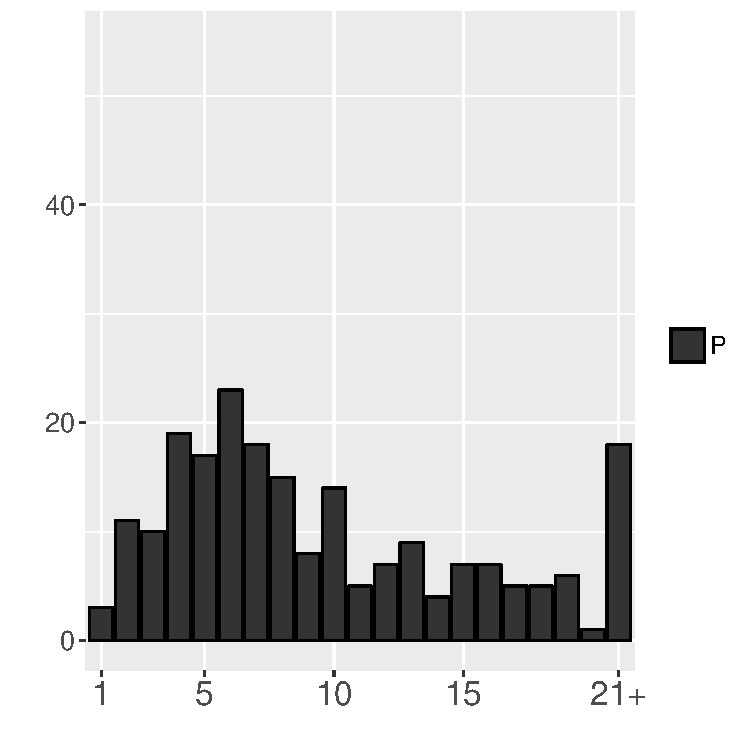
\includegraphics[width=0.6\textwidth]{figure/WOPNew.pdf}
	\caption{Word order of non-anaphoric P}
	\label{WOPNewF}
	\end{center}
%\end{minipage}
\end{figure}

%%----------------------------------------------------
\subsubsection{Pronouns appear clause-initially}\label{WO:ClauseInit:Ident:Pron}

Next let us examine the position of pronouns.
Figure \ref{WOExpTypeF} shows the positions of pronouns.
Figure \ref{DEPositionAllF}, repeated as Figure \ref{DEPositionAllF2} for comparison,
represents the distributions of all elements.
Although the number of pronoun is small,
it is clear, comparing with the overall distributions of elements in Figure \ref{DEPositionAllF2}, that
the order of pronouns is skewed to earlier positions within a clause.
Hence, it is reasonable to conclude that
pronouns are likely to appear earlier in a clause.
Examples of pronouns appearing earlier in a clause are shown in \ref{PronIni1} and \ref{PronIni2} above.
The result is compatible with \citeA{yamashita02} and \citeA{kondoyamashita07}.


\begin{figure}
%\begin{minipage}{0.5\textwidth}
	\begin{center}
	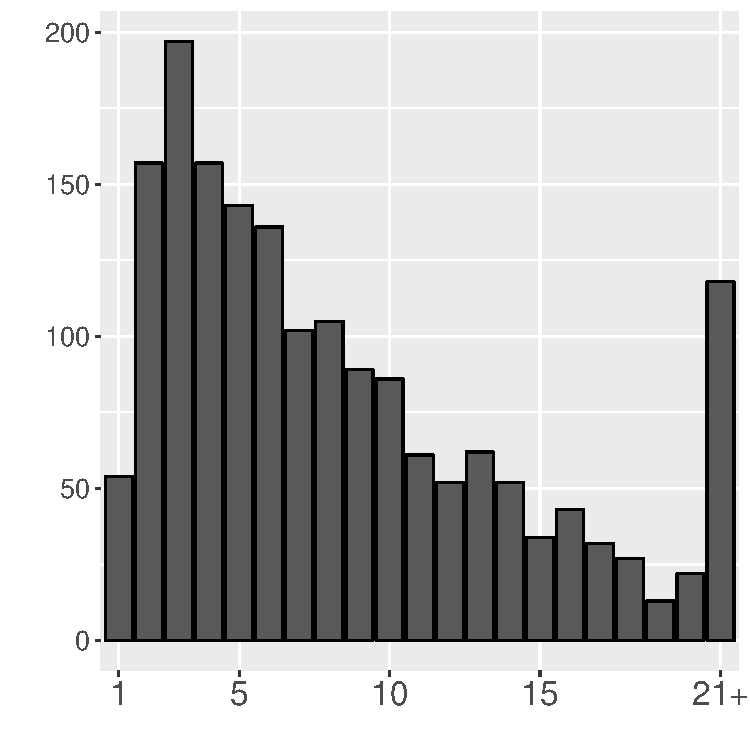
\includegraphics[width=0.6\textwidth]{figure/DEPositionAll.pdf}
	\caption{Order of all elements}
	\label{DEPositionAllF2}
	\end{center}
%\end{minipage}
\end{figure}
\begin{figure}
%\begin{minipage}{0.5\textwidth}
	\begin{center}
	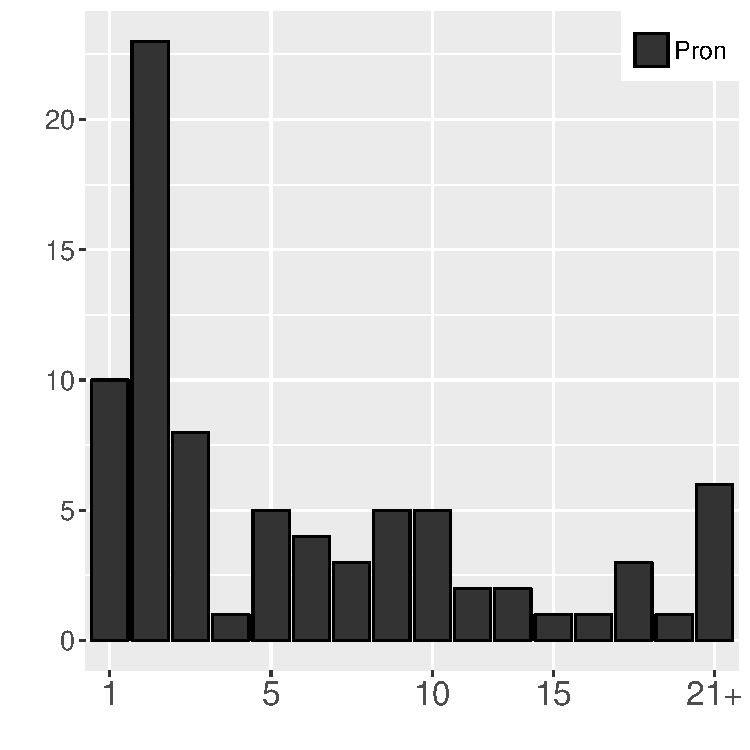
\includegraphics[width=0.6\textwidth]{figure/WOExpType.pdf}
	\caption{Order of pronouns}
	\label{WOExpTypeF}
	\end{center}
\end{figure}

%\begin{table}
%\begin{minipage}{0.5\textwidth}
%\centering
%	\caption{Markers for ASP (given)}
%	\label{ASPParGivenT}
%	\begin{tabular}{lrrr}
%	\toprule
%			 & A & S & P \\
%	\midrule
%	\ci{o} 	& 0 & 0 & 166 \\
%	\ci{ga} 	& 29 & 191 & 0 \\
%	\midrule
%	case marker & 29 & 191 & 166 \\
%	  & (50.9\%) & (59.0\%) & (91.2\%) \\
%	\midrule
%	\midrule
%	\ci{wa} 	& 27 & 104 & 14 \\
%	\ci{toiunowa} 	& 1 & 29 & 2 \\
%	\midrule
%	topic marker & 28 & 133 & 16 \\
%	  & (49.1\%) & (41.0\%) & (8.8\%) \\
%	\midrule
%	\midrule
%	sum & 57 & 324 & 182 \\
%	  & (100\%) & (100\%) & (100\%) \\
%	\bottomrule
%	\end{tabular}
%\end{minipage}
%\begin{minipage}{0.5\textwidth}
%\centering
%	\caption{Markers for ASP (new)}
%	\label{ASPParNewT}
%	\begin{tabular}{rrr}
%	\toprule
%	A & S & P \\
%	\midrule
%	0 & 0 & 211 \\
%	15 & 351 & 0 \\
%	\midrule
%	15 & 351 & 211 \\
%	(78.9\%) & (76.5\%) & (92.5\%) \\
%	\midrule
%	\midrule
%	3 & 90 & 14 \\
%	1 & 18 & 3 \\
%	\midrule
%	4 & 108 & 17 \\
%	(21.1\%) & (23.5\%) & (7.5\%) \\
%	\midrule
%	\midrule
%	19 & 459 & 228 \\
%	(100\%) & (100\%) & (100\%) \\
%	\bottomrule
%	\end{tabular}
%\end{minipage}
%\end{table}

%%----------------------------------------------------
\subsubsection{Unused elements appear clause-initially}\label{WO:ClauseInit:Ident:ActStatus}

Not only evoked, inferable, and declining elements,
unused elements appear clause-initially.
Elements coded by copula followed by \ci{ga} or \ci{kedo} are unused elements as has been discussed in Chapter \ref{Particles}.%
 \footnote{
 \chd{See \S \ref{BackSubSubKedo} for the reason why
 An element coded by copula followed by \ci{ga} or \ci{kedo} is not considered to be a clause.}
 }
It is very unnatural when they are preceded by other arguments.
For example,
as shown in the contrast between \Next[a] and \Next[b],
\ci{rei-no ken} `that issue' cannot be felicitously preceded by another argument, in this case \ci{kotira-de} `this side'.
%
\ex.
 \ag. \EM{rei-no} \EM{ken-desu-ga} kotira-de nantoka nari-sou-desu \\
      that-\ab{gen} issue-\ab{cop}.\ab{plt}-though this.side-\ab{loc} whatever become-will-\ab{cop}.\ab{plt} \\
      `Regarding that issue, (I) guess (we) figured the way out.'
      \hfill{\cite[modified from][283]{niwa06}}
 \bg.[a$^{\prime}$.] ??kotira-de \EM{rei-no} \EM{ken-desu-ga} nantoka nari-sou-desu \\
      this.side-\ab{loc} that-\ab{gen} issue-\ab{cop}.\ab{plt}-though whatever become-will-\ab{cop}.\ab{plt} \\

In a similar manner,
\ci{yamada-no koto} `the issue of Yamada' cannot naturally be preceded by adverbial, \ci{ano mama} `that way'
as shown in the contrast between \Next[a] and \Next[b].
%
\ex.
 \ag. \EM{yamada-no} \EM{koto-da-kedo} ano mama hot-toi-te ii-no-kana \\
      Yamada-\ab{gen} issue-\ab{cop} that way leave-let-and good-\ab{nmlz}-\ab{q} \\
      `Regarding Yamada, is it OK to just leave him?'
      \hfill{\cite[283]{niwa06}}
 \bg.[a$^{\prime}$.] ??ano mama \EM{yamada-no} \EM{koto-da-kedo} hot-toi-te ii-no-kana \\
      that way Yamada-\ab{gen} issue-\ab{cop} leave-let-and good-\ab{nmlz}-\ab{q} \\


Unused elements include indefinite elements
although it is counter-intuitive to consider indefinite NPs as being ``shared''.
For example, as has been mentioned in \S \ref{Fr:Definition:TFFeathers:Definite},
an indefinite element can appear clause-initially
if the speaker assumes the hearer to remember that the speaker (or somebody else) has talked about a category the element refers to.
For example, as shown in \Next[Y],
repeated from \ref{Fr:Definition:TFFeathers:Definite:Ex:Mango1} in \S \ref{Fr:Definition:TFFeathers:Definite},
having mentioned a category of mango makes it possible for \ci{mangoo} `mango' to appear clause-initially,
even though
\ci{mangoo} `mango' is clearly indefinite
since the hearer has no way to tell which mango the speaker ate.
I regard this as unused and hence shared.
%
\ex. Context:
	Y told H that he had never seen and eaten mangoes.
	H told Y that they are delicious.
	Several days later, Y finally ate a mango.
	\ag.[Y:] \EM{mangoo} konoaida miyako-zima-de tabe-ta-yo \\
			mango the.other.day Miyako-island-\ab{loc} eat-\ab{past}-\ab{fp} \\
			`(I) ate (a) mango (we talked about) in Miyako island the other day.'
	\bg.[Y$^{\prime}$:] konoaida miyako-zima-de \EM{mangoo} tabe-ta-yo \\
			the.other.day Miyako-island-\ab{loc} mango eat-\ab{past}-\ab{fp} \\
			`(I) ate (a) mango in Miyako island the other day.'

In this case, however,
\ci{mangoo} `mango' in the pre-predicate position is also felicitous
as in \Last[$^{\prime}$],
which indicates that this is a borderline case;
\ci{mangoo} can be a topic in the sense that
it is unused and the speaker has talked about before,
while it can be a focus in the sense that
it is new to the discourse and indefinite.

On the other hand, in \Next[Y],
%repeated from (\ref{Fr:Definition:TFFeathers:Definite:Ex:Mango2}),
where the speaker does not assume the hearer to remember that
the speaker has talked about mango,
clause-initial \ci{mangoo} `mango' is infelicitous,
whereas pre-predicate \ci{mangoo} is perfectly acceptable.
%
\ex. Context:
	Y and H have not met for a few months.
	\a.[H:] What did you do these days?
	\bg.[Y:] ??\EM{mangoo} konoaida miyako-zima-de tabe-ta-yo \\
			mango the.other.day Miyako-island-\ab{loc} eat-\ab{past}-\ab{fp} \\
		\hfill(=\LLast[Y])
	\bg.[Y$^{\prime}$:] konoaida miyako-zima-de \EM{mangoo} tabe-ta-yo \\
			the.other.day Miyako-island-\ab{loc} mango eat-\ab{past}-\ab{fp} \\
			`(I) ate (a) mango in Miyako island the other day.'
		\hfill(=\LLast[Y$^{\prime}$])

Therefore, it is reasonable to conclude that
shared elements include those which refer to categories the speaker (or somebody else) has talked about and that
they can appear clause-initially.


%%----------------------------------------------------
\subsection{Persistent elements tend to appear clause-initially}\label{PersistentAppearClause-Initially}

Persistent elements are skewed to earlier positions than non-persistent elements
as shown in Figure \ref{DEPositionPerF}.
%This is especially clear in the contrast between Figure \ref{WOASPPerF} and \ref{WOASPNPerF},
%which show the word order of A, S, and P for persistent and non-persistent elements
%in a clause which contains more than one argument.
%Most Exs and As are persistent and precede other arguments as in Figure \ref{WOASPPerF} compared to Figure \ref{WOASPNPerF}.

%\begin{figure}
%\begin{minipage}{0.5\textwidth}
%	\begin{center}
%	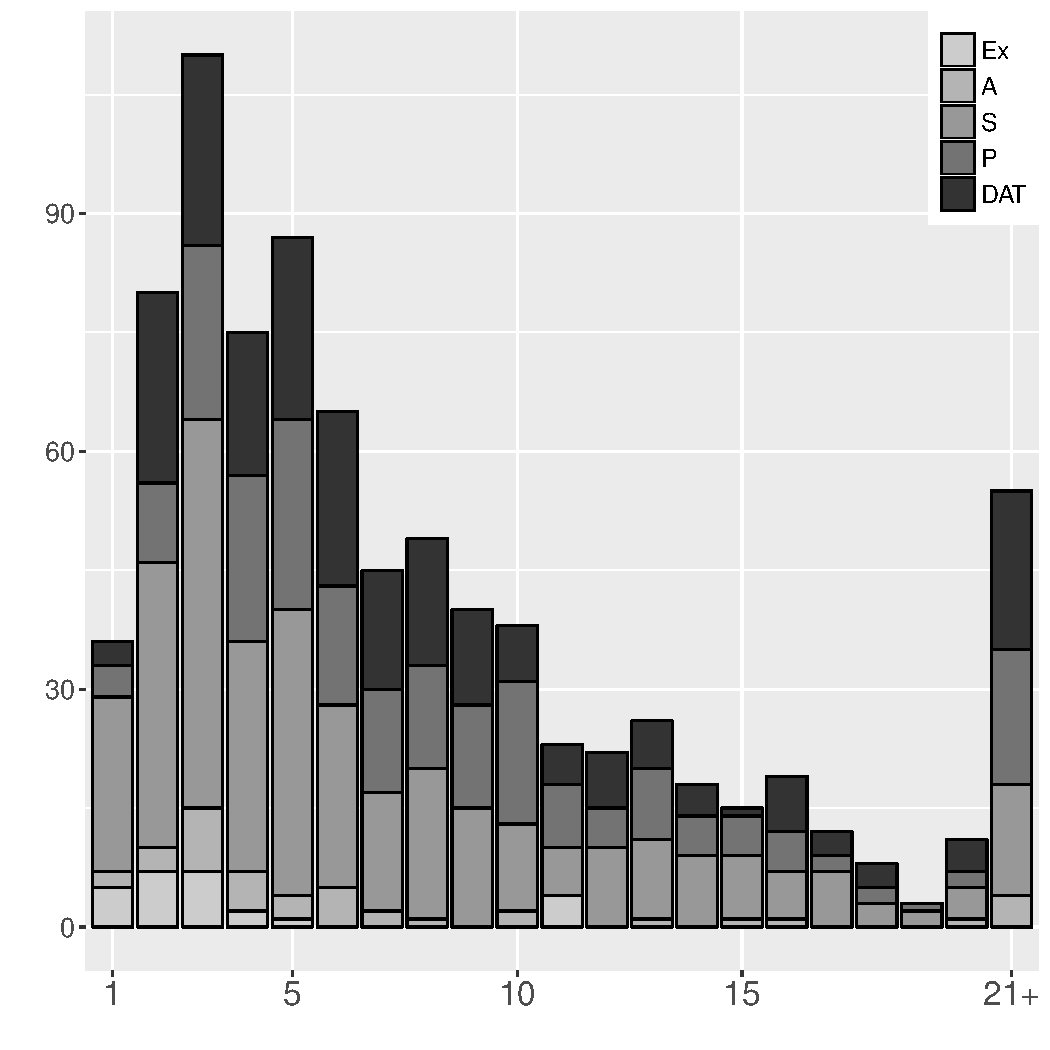
\includegraphics[width=0.95\textwidth]{figure/WOASPPer.pdf}
%	\caption{Word order vs.\ grammatical function (persistent)}
%	\label{WOASPPerF}
%	\end{center}
%\end{minipage}
%\begin{minipage}{0.5\textwidth}
%	\begin{center}
%	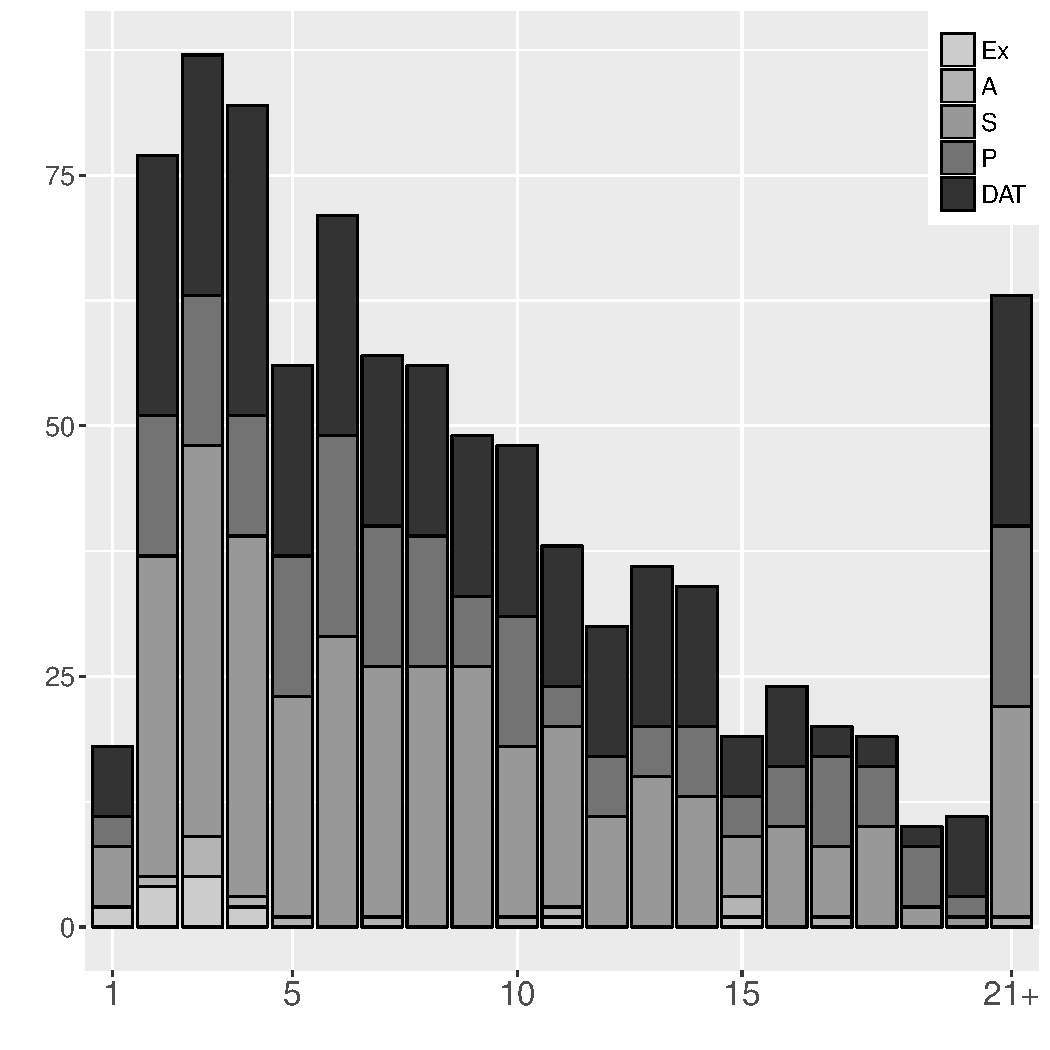
\includegraphics[width=0.95\textwidth]{figure/WOASPNPer.pdf}
%	\caption{Word order vs.\ grammatical function (non-persistent)}
%	\label{WOASPNPerF}
%	\end{center}
%\end{minipage}
%\end{figure}
The following are examples of persistent elements appearing clause-initially.
In \Next,
\ci{hihu-byoo} `skin-disease' in line a, coded by the topic marker \ci{toiuno-wa},
appear clause-initially.
The predicate appear in line c,
intervened by a proposition in line b and also another argument (\ci{hito-ni} `person-by') of the clause.
Also in line d, \ci{kore-wa} `this-\ci{wa}', referring to `skin-disease', appear clause initially.
%
\ex.
 \ag. \EM{hihu-byoo-toiuno-wa} \\
 		skin-disease-\ci{toiuno-wa} \\
		`The skin disease,'
 \bg. damat-tei-temo \\
 		keep.silent-\ab{prog}-even.if \\
		`even if you don't tell people about it,'
 \bg. hito-ni \ul{mir-are-te-simau} mono-dat-ta-node \\
 		person-by see-\ab{pass}-and-\ab{pfv} thing-\ab{cop}-\ab{past}-because \\
		`people can see it, so'
 \bg. \EM{kore-wa} ano omot-ta izyooni seesintekini \ul{kutuu-desi}-ta \\
 		this-\ci{wa} \ab{fl} think-\ab{past} more mentally painful-\ab{cop}-\ab{past} \\
		`this was mentally painful more than I had expected.'
		\hfill{(\code{S02F0100: 222.75-231.09})}
%S02F0100|00222751L|222.750605|231.088045|L|皮膚病というのは(0.428)黙っていても(0.285)人に見られてしまうものだったので(0.429)これは(F あの)思った以上に精神的に苦痛でした|[文末]|

Similarly, in \Next,
\ci{sore-wa} `that-\ci{wa}' in line b and g,
and \ci{sore-dake-wa} `that-only-\ci{wa}' in line i,
all of which refer to `chelow kebab' in line a,
appear clause-initially.
%
\ex.
 \a. There is a dish called \EM{chelow kebab}.
 \bg. de \EM{sore-wa} eeto gohan-ni eeto bataa-o maze-te \\
 	and that-\ci{wa} \ab{fl} rice-to \ab{fl} butter-\ci{o} mix-and \\
	`That, you mix rice with butter...'
 \b. on top of that you put spice,
 \b. on top of that you put mutton,
 \b. you mix it and eat it.
 \b. There were many dishes of this kind.
 \bg. \EM{sore-wa} kekkoo sonnani hituzi-no oniku-no kusasa-mo naku-te \\
 	that-\ci{wa} to.some.extent not.really sheep-\ab{gen} meat-\ab{gen} smell-also not.exist-and \\
	`It did not have smell of mutton...'
 \b. I thought it was delicious.
 \bg. \EM{sore-dake-wa} anoo iran-ryoori-no naka-de \ul{taberu} koto-ga ano deki-ta ryoori-desu \\
 		that-only-\ci{wa} \ab{fl} Iran-dish-\ab{gen} inside-\ab{loc} eat thing-\ci{ga} \ab{fl} can-\ab{past} dish-\ab{cop} \\
		`This is the only dish I could eat among Iran dish.'
 \hfill{(\code{S03F0072: 446.03-447.66})}
%S03F0072|00446026L|446.026013|447.663208|L|チェロカバブというのがありまして|/テ節/|
%S03F0072|00448150L|448.150018|463.667799|L|でそれは(0.114)(F えーと)御飯に(0.376)(F えーと)バターを混ぜてその上に香辛料を振って(0.174)その上に羊のお肉が乗っていて(0.289)それをこう(0.11)混ぜてぐちゃぐちゃに混ぜて食べるという(0.441)(F えーと)お料理が(0.707)(F あのー)(0.681)多かったんですけれども|/並列節ケレドモ/|
%S03F0072|00464361L|464.360734|476.870208|L|それは結構そんなに羊の(0.42)お肉の臭さもなくて(1.094)(F あのー)(0.156)おいしいな(0.178)って(0.418)思ってそれだけは(0.475)(F あのー)イラン料理の中で(0.273)食べることが(0.28)(F あの)できた料理です|[文末]|

\chd{As has been mentioned in \ref{WO:Intro},
both word order and particles significantly contribute to predict persistence,
contrary to the result of \citeA{imamura17},
who concludes that ``scrambling [PSV order] is pertinent to anaphorically prominent but cataphorically non-prominent objects and that topicalization is especially germane to `continuing topic' as the referent of the object'' (p.~78).
There are a few potential reasons for why the results of the present work are different from those of \citeA{imamura17}.
One potential reason is the difference of modalities;
\citeA{imamura17} employed a corpus of written Japanese (\ci{the Balanced Corpus of Contemporary Written Japanese}, BCCWJ), while the present study employs spoken Japanese.
Related to the first point,
clause-chaining, which I will point out is one of the motivations for clause-initial elements tend to be persistent (see the next section),
only appears in spoken Japanese, but not in written Japanese.
In any case, this is a mere speculation and further studies are needed to analyze
why the results of two studies differ.}


%%----------------------------------------------------
\subsection{Motivations for topics appearing clause-initially}\label{TopicAppearClause-Initially}

As has been pointed out by many linguists,
topics tend to appear clause-initially
because they function as an anchor of the previous discourse.
The principle \ref{oldnewprinciple} is motivated by this processing convenience \cite[e.g.,][]{keenan77}.
Clause-initial locatives and other adjectives can be also explained by this motivation.
This anchoring function best works when the activation cost of the referent is relatively high \cite{givon83};
i.e.,
when the referent of the element in question is inferable or declining.
When the activation cost is low, i.e., the topic is continuous from the previous discourse,
the element in question that refers to the topic is expected to be zero \cite{givon83,gundeletal93,ariel90};
there is no need for anchoring because the topic is already evoked and the hearer expects the topic to be also mentioned in the current sentence.
This explanation predicts that the distance between the element in question and the antecedent is larger when the element in question is expressed in the form of NP instead of zero.
Figure \ref{DistExpTypeF} appears to support this prediction,
\chd{although a statistical analysis indicates that the expression types do not significantly contribute to predict the distance.
This paragraph discuss NPs with long distance.
See the discussion below for NPs with shorter distance.}
The whisker plot in FIgure \ref{DistExpTypeF} shows the distance between the element in question (NP vs.\ (explicit) pronoun vs.\ zero pronoun) and its antecedent.
It measures the time between when the first mora of the element question is produced and when the first mora of the antecedent produced.
The figure shows that the distance between NP and the antecedent is larger than that of zero and the antecedent in many cases.
Zero pronouns are assumed to be produced at the time
when the first mora of the predicate is uttered.

\Next exemplifies this pattern,
\chd{where zero pronouns are indicated by \ci{\O}.}
In line b, \ci{san-nin-me} `the last person' precedes adjuncts (`last fall') and coded by a variation of \ci{toiuno-wa} (\ci{ttuuno-wa}).
\chd{Zero pronouns \ci{\O} are inserted right before the predicate for the purpose of presentation,
but this does not affect the analysis.}
Since this person is one of the three people mentioned in line a,
this person is inferable
through a part-whole relation.
The topic moves on to another person in line f, who is also one of the three people mentioned in line a.
In line j, the speaker again refers to the person mentioned in line b.
Also this time, the element \ci{moo hitori-wa} `the other person' appears near clause-initially, preceding other arguments.
The referent keeps to be mentioned until line q.
%where the elements that refer to this person is either pronouns, as in line h and k, or zero, as in line i, l, and o.
Finally, the speaker starts talking about himself in line r,
in which case the element \ci{boku-wa} `\ab{1}\ab{sg}-\ci{wa}' appear near clause-initially.
%
\ex.
 \a. All of us three quitted this job, interestingly, or strangely.
 \bg. de anoo \EM{san-nin-me-ttuuno-wa} tui se ee kyonen-no o aki-ni yame-ta-n-desu-kedomo \\
 	and \ab{fl} three-\ab{cl}-\ab{ord}-\ci{toiuno}-\ci{wa} just \ab{frg} \ab{fl} last.year-\ab{gen} \ab{fl} fall-in quit-\ab{past}-\ab{nmlz}-\ab{cop}.\ab{plt}-though \\
	`The last person quitted this fall.'
 \bg. \EM{soitu-wa} maa itiban saisyo-ni yame-tai yame-tai ttut-ta ningen-nan-desu-kedomo \\
 		\ab{3}\ab{sg}-\ci{wa} \ab{fl} most first-in quit-want quit-want \ab{quot}.say-\ab{past} person-\ab{nmlz}-\ab{cop}.\ab{plt}-though \\
		`He was the first person who said he wanted to quit.'
 \b. This kind of thing often happens.
 \b. All of us three quitted eventually.
 \bg. ndee \ul{hitori-wa}-desu-ne \\
 		then one.person-\ci{wa}-\ab{cop}.\ab{plt}-\ab{fp} \\
		`Concerning another person,'
 \b. I guess this is closely related to the fact that we worked in Mobara.
 \bg. de hitotu \ul{sono} \ul{hito-wa} ee ma yappari tonikaku hatarai-te okane-ga koo te-ni \EM{\O} hairu-tte iu koto-ni itiban-no kati-o miidasi-ta wake-desu-ne sono ziki-ni \\
 		then one.thing that person-\ci{wa} \ab{fl} \ab{fl} as.expected any.way work-and money-\ci{ga} this.way hand-to {\O} get.in-\ab{quot} say thing-to most-\ab{gen} value-\ci{o} find-\ab{past} reason-\ab{cop}.\ab{plt}-\ab{fp} that time-at \\
		`At that time this person found it most valuable to work hard and gain money.'
 \b. (Explanation about his view on working. 9.3 sec.)
 \bg. de moo \EM{hitori-wa} maa \EM{kare-mo} hi hizyooni mobara-o aisi-teru-n-desu-ga \\
 	then more one.person-\ci{wa} \ab{fl} \ab{3}\ab{sg}.\ab{m}-also \ab{frg} very Mobara-\ci{o} love-\ab{prog}-\ab{nmlz}-\ab{cop}.\ab{plt}-though \\
	`The other one, who also loves Mobara (a place name),'
 \bg. kondo-no sigoto-tte atarasiku \EM{\O} tui-ta sigoto-tteiuno-wa \\
 		next-\ab{gen} job-\ab{quot} newly {\O} acquire-\ab{past} job-\ci{toiuno}-\ci{wa} \\
		`(his) next job, the new job (he) acquired is...'
 \bg. maa inaka-no hoo-no sigoto-nan-desu-ne \\
 	\ab{fl} rural-\ab{gen} area-\ab{gen} job-\ab{nmlz}-\ab{cop}.\ab{plt}-\ab{fp} \\
	`in rural area.'
 \bg. de \EM{kare} iwaku-desu-ne \\
 	then \ab{3}\ab{sg}.\ab{m} say-\ab{plt}-\ab{fp} \\
	`According to what he says,'
 \bg. sono yama-ga nai tokoro-ni-wa \EM{\O} sum-e-nai-to \\
 	\ab{fl} mountain-\ci{ga} not.exist place-at-\ci{wa} {\O} live-can-\ab{neg}-\ab{quot} \\
 	`He says that he cannot live in places without mountains.'
 \b. Though Mobara does not have mountains, the sky in Mobara is clear.
 \b. We call it Mobara sky. Mobara has such an idyllic scene.
 \bg. sore-ga maa doositemo nai-to \EM{\O} sum-e-nai-tte iu koto-o sono ziki-ni \EM{\O} sato-ta-n-zya-nai-ka-to \\
 	that-\ci{ga} \ab{fl} by.all.means not.exist-\ab{cond} {\O} live-can-\ab{neg}-\ab{quot} say thing-\ci{o} that time-in {\O} learn-\ab{past}-\ab{nmlz}-\ab{cop}-\ab{neg}-\ab{q}-\ab{quot} \\
	`(He) learned at that time that (he) can't live without such scene (I guess).'
 \b. de \ul{\ul{boku-wa}}-to ii-masu-to \\
 	then \ab{1}\ab{sg}-\ab{quot} say-\ab{plt}-\ab{cond} \\
	`Talking about myself...'
 \b. ...
   \hfill{(\code{S05M1236: 639.40-738.22})}
%S05M1236|00639399L|639.399427|647.222898|L|て(0.466)(F まー)これがまた(?)(0.115)(F あのー)(0.273)不思議なことにと言うか(0.211)<咳>面白いことにその三人共ですねその会社を(0.187)(F えー)(0.378)辞めました|[文末]|
%S05M1236|00647283L|647.283|653.466794|L|<笑>で(0.587)(F あのー)三人目っつうのはつい(D せ)(F えー)去年の(0.222)(D (? お))秋に辞めたんですけども|/並列節ケドモ/|
%S05M1236|00653467L|653.466794|656.353546|L|そいつは(F まー)一番最初に辞めたい辞めたいっつった人間なんですけども|/並列節ケドモ/|
%S05M1236|00656478L|656.47798|657.577155|L|えてしてそういうもんですが|/並列節ガ/|
%S05M1236|00658101L|658.101232|660.387564|L|(F えー)(0.742)三人共辞めました|[文末]|
%S05M1236|00660711L|660.710985|667.679344|L|んで一人はですね(0.671)(F えー)(0.238)(F ま)これやっぱり茂原で働いたっていうことに大きく関係してそうなんですねその辞めた理由っていうのが||倒置−つなぎ切り
%S05M1236|00667930L|667.930126|678.94475|L|で一つ(D い)その人は(0.608)(F えー)(0.293)(F ま)やっぱり(0.376)とにかく(0.172)働いてお金がこう手に入るっていうことに(0.215)一番の価値観を(0.47)見出だした訳ですねその(0.157)その(D 時)(F えー)時期に||倒置−つなぎ切り
%S05M1236|00679812L|679.811821|689.132829|L|それで今でもですね(0.563)(F まー)(0.166)一番お金が(0.132)入るところっていうんで(0.267)色々職を転々として(0.54)(F まー)(0.294)相当金持ちに(0.284)なってるようですけども|/並列節ケドモ/|
%S05M1236|00689447L|689.446897|694.030141|L|(F まー)一つの生き方かなと(0.427)いう風に(0.372)(F えー)(0.685)僕なんかも見てますけども|/並列節ケドモ/|
%S05M1236|00694880L|694.880285|707.26424|L|でもう一人は(0.959)(F まー)(0.656)彼も(D (? ひ))非常に茂原を愛してるんですが(0.285)(F えー)(0.466)(F ま)今度の仕事っていうのは(0.473)(F あのー)(0.294)今度の仕事って新しく就いた仕事っていうのは(0.39)(F まー)田舎の方(D2 で)(0.275)(F えー)の仕事なんですね|[文末]|
%S05M1236|00708165L|708.164927|711.5187|L|で彼曰くですね(0.192)(F その)山がないところには住めないと|[と文末]|
%S05M1236|00711927L|711.927|728.390145|L|<笑>で茂原ってのは(F まー)山がある訳じゃないんだけど(0.393)(F あのー)(0.308)非常に澄み切った(0.517)(F えー)空でそれのことを(0.24)(F あのー)僕ら茂原晴れと言ってるんですけども(0.602)(F えー)(F まー)(D 非)非常に(F あのー)(0.697)(F まー)(0.215)そういう(0.561)のどかな風景がある訳ですね|[文末]|
%S05M1236|00729305L|729.305466|734.964084|L|で(0.259)<咳>(0.75)それが(F まー)どうしてもないと住めないっていうことをその時期に悟ったんじゃないかと|[と文末]|
%S05M1236|00736425L|736.425057|738.218691|L|で(0.664)僕はと言いますと|/条件節ト/|
%S05M

In this type of example,
clause-initial elements especially coded by topic markers function as an anchor to the previous discourse.

\begin{figure}
%\begin{minipage}{0.5\textwidth}
	\begin{center}
	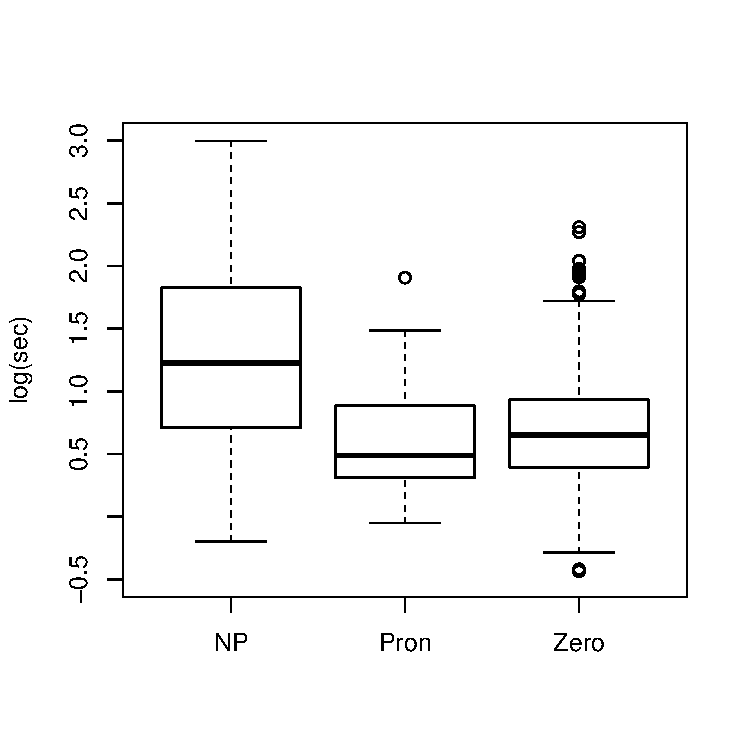
\includegraphics[width=0.5\textwidth]{figure/DistExpType.pdf}
	\caption{Anaphoric distance vs.\ expression type}
	\label{DistExpTypeF}
	\end{center}
%\end{minipage}
\end{figure}


However,
Figure \ref{DistExpTypeF} also indicates that
(explicit) pronouns (\ci{kore} `\ab{dem}.\ab{prox} (this)', \ci{sore} `\ab{dem}.\ab{med} (this/that)', \ci{are} `\ab{dem}.\ab{dist} (that)', \ci{kare} `\ab{3}\ab{sg}.\ab{m} (he)', \ci{kanozyo} `\ab{3}\ab{sg}.\ab{f} (she)')%
	\footnote{
	\ci{Kare} `\ab{3}\ab{sg}.\ab{m} (he)' and \ci{kanozyo} `\ab{3}\ab{sg}.\ab{f} (she)' are very rare in spoken Japanese.
	Instead, \ci{kono hito} `this person' or similar expressions are used more frequently.
	However, this study does not count them as pronouns.
	}
and zero pronouns do not differ from each other.
%Or pronouns even seem to have shorter distance than zeros.
Moreover, there are NPs which refer to the immediate antecedent;
\chd{Whereas more than half of the NPs have longer distance than explicit and zero pronouns,
the figure also shows that many NPs have distance as short as that explicit and zero pronouns.
In fact, a fixed effects analysis for the distance (the expression type as a fixed effect and the speaker as a random effect) indicates that expression types are not a significant factor to predict the distance.}
For example, in the previous example \Last,
the referent of \ci{hitori} `one person' in line f is mentioned in line h as \ci{sono hito} `that person' again,
although the distance is not very far.%
	\footnote{
	The impression of line g is inserted clause rather than topic shift.
	}
In a similar manner,
the referent of \ci{san-nin-me} in line b is mentioned immediately following clause (line c) as \ci{soitu} `\ab{3}\ab{sg}'.
These examples are not mere exceptions.
in fact, 74.1\% of secondly mentioned referents are still expressed in the form of NP;
only 21.4\% are expressed as zero and 4.6\% as pronoun
as shown in Table \ref{AnaCountExpTypeT} and Figure \ref{AnaCountExpTypeF}.
Figure \ref{AnaCountExpTypeF} and Table \ref{AnaCountExpTypeT} show
the expression type of the element in question based on how many times the referent is mentioned.
"2" indicates that the element in question is second mentioned,
"3" indicates that it is third mentioned, and so on.
The ratio of zero increases as the referent keeps to be mentioned.
The fact that the referent introduced is mentioned repeatedly is also reported in \citeA{clancy80}, who investigates Pear Stories;
this pattern is not unique to the corpus of the current study.
\Next is another example
of two NPs which refers to the same referent adjacent with each other.
In this example,
the very long word \ci{yuugosurabia-syakaisyugi-kyoowakoku} `Socialist Federal Republic of Yugoslavia' is repeated twice.
%
\ex.\label{WO:TopicAppearClause-Initially:Ex:Yuugo}
 \ag. ee kon ma kono tiiki ee yu ma \EM{kyuu-yuugosurabia-syakaisyugi-kyoowakoku}-toiu tokoro-nan-desu-keredomo \\
 	\ab{fl} \ab{frg} \ab{fl} this area \ab{fl} \ab{frg} \ab{fl} former-Yugoslavia-socialist-republic-\ab{quot} place-\ab{nmlz}-\ab{cop}.\ab{plt}-though \\
	`This area is called Socialist Federal Republic of Yugoslavia,'
 \bg. kono \EM{yuugosurabia-syakaisyugi-kyoowakoku}-tteiuno-wa motomotoga ee minzoku-tairitu-no hagesii tiiki-de-gozai-masi-te \\
 	this Yugoslavia-socialist-republic-\ci{toiuno}-\ci{wa} originally \ab{fl} ethnic-conflict-\ab{gen} severe area-\ab{cop}-\ab{plt}-\ab{plt}-and \\
	`this Socialist Federal Republic of Yugoslavia is an area with severe ethnic conflicts...'
	\src{S00M0199: 81.95-94.42}
%S00M0199|00081950L|81.949813|94.424971|L|(F えー)(0.143)(D こん)(F ま)この地域(F えー)(D ユ)(0.253)(F ま)旧ユーゴスラビア社会主義共和国というところなんですけれども(0.426)このユーゴスラビア社会主義共和国っていうのは元々が(0.26)(F えー)民族対立の激しい地域でございまして|/テ節/|
%S00M0199|00094875L|94.874776|96.351778|L|(F えー)(0.217)(F ま)一つの||言いさし−言い直しあり
%S00M0199|00096450L|96.449668|124.995828|L|(F えー)(F え)戦後(F えー)第二次大戦終了後(0.115)(F おー)から言われてた言葉として(0.418)(F えー)(D ひ)一つの(0.152)(F えー)(D す)(F ま)政党ですね共産党が支配する(0.418)(F えー)二つの(0.152)(F えー)(F ま)二つの(0.108)(F え)言葉(F え)(F う)(0.196)文字を持ち(0.438)三つの宗教があり(0.219)(F えー)四つの(0.132)(F えー)言語を話す(0.471)で五つの(F えー)民族によって構成される(0.434)国と言われる(F まー)(0.447)(F えー)歴史的に見ても類い稀な(F あ)(F えー)モザイク国家と(0.282)いうことだったんですが|/並列節ガ/|

Why does the speaker repeat the same referent adjacent with each other,
although s/he can fairly assume that the referent has been already evoked by the first mention?
In fact, the second `Socialist Federal Republic of Yugoslavia' in line b cannot be omitted contrary to what is claimed about the nominal forms \cite{givon83,gundeletal93,ariel90}.
Why?

\begin{table}
	\centering
	\tblcaption{Nth mention vs.\ expression type}
	\begin{tabular}{lrrrrr}
	\toprule
          &  2  & 3   &  4 & 5  & 6+ \\
    \midrule
  NP      & 260 & 135 & 83 & 54 & 255 \\
          & \rt{(74.1\%)} & \rt{(64.9\%)} & \rt{(58.0\%)} & \rt{(52.4\%)} & \rt{(40.5\%)} \\
  Pronoun & 16  & 14  & 9  & 13 & 20 \\
          & \rt{(4.6\%)} & \rt{(6.7\%)} & \rt{(6.3\%)} & \rt{(12.6\%)} & \rt{(3.2\%)} \\
  Zero    & 75  & 59  & 51 & 36 & 355 \\
          & \rt{(21.4\%)} & \rt{(28.4\%)} & \rt{(35.7\%)} & \rt{(35.0\%)} & \rt{(56.3\%)} \\
    \midrule
  Sum     & 351 & 208 & 143 & 103 & 630 \\
          & \rt{(100\%)} & \rt{(100\%)} & \rt{(100\%)} & \rt{(100\%)} & \rt{(100\%)} \\
    \bottomrule
	\end{tabular}
	\label{AnaCountExpTypeT}
%\end{table}
%         2   3   4   5  6+
%  NP   260 135  83  54 255
%  Pron  16  14   9  13  20
%  Zero  75  59  51  36 335
\end{table}

\begin{figure}
	\centering
	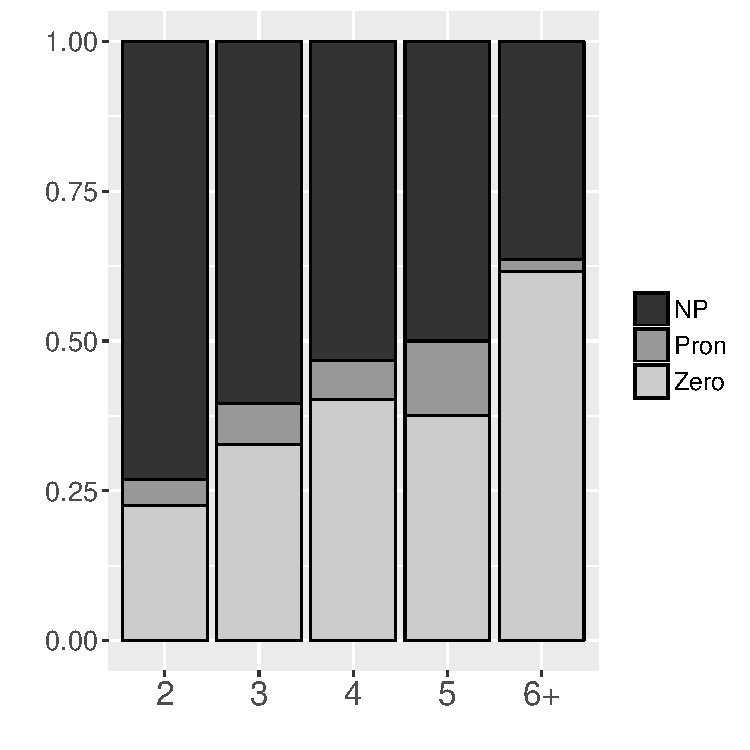
\includegraphics[width=0.5\textwidth]{figure/AnaCountExpType.pdf}
	\caption{Nth mention vs.~expression type}
	\label{AnaCountExpTypeF}
\end{figure}

Since the most frequent pronouns is zero pronoun in Japanese as indicated in Figure \ref{AnaCountExpTypeF} and Table \ref{AnaCountExpTypeT},
the speaker needs to make sure that the hearer understand which referent zero pronouns refer to.
Therefore, the speaker needs to establish the referent as a topic
before s/he uses zero.%
 \footnote{\chd{
 As pointed by one of the reviewers (Morimoto),
 it is possible to replace `this Socialist Federal Republic of Yugoslavia' in line b of \ref{WO:TopicAppearClause-Initially:Ex:Yuugo} with pronoun-like form such as \ci{kono kuni} `this country'.
 My argument here still holds because the pronoun-like form `this country' is
 much more informative than zero pronoun.
 The following argument by \citeA{lambrecht94} also suggests that
 focus can be the antecedent of overt pronouns, but not zero pronouns.
 See examples \ref{WO:TopicAppearClause-Initially:Ex:John} and \ref{WO:TopicAppearClause-Initially:Ex:Rosa}.
 }}
This might be related to the observation in \citeA[p.~136]{lambrecht94} that
focus elements cannot be the antecedent of zero,
while topic elements can.
Compare \Next and \NNext (the acceptability judgements are based on Lambrecht. Information structure is added by the present author).
In \Next, \ci{John} is interpreted as topic (by default) in \Next[b],
in which case zero is acceptable.
%
\ex.\label{WO:TopicAppearClause-Initially:Ex:John}
 \a. John married Rosa, but he didn't really love her.
 \b. [John]$_{T}$ [married Rosa]$_{F}$, but {\O} didn't really love her.

On the other hand,
in \Next,
\ci{John} is focus because it is the answer to the question,
in which case zero is not acceptable as in \Next[b].
Only explicit pronoun is acceptable as shown in \Next[a].
%
\ex.\label{WO:TopicAppearClause-Initially:Ex:Rosa}
 \a.[Q:] Who married Rosa?
 \b.[A:]
   \a.[a.] John married Rosa, but he didn't really love her.
   \b.[b.] *?[John]$_{F}$ [married Rosa]$_{T}$, but {\O} didn't really love her.


\begin{figure}
%\begin{minipage}{0.5\textwidth}
	\begin{center}
	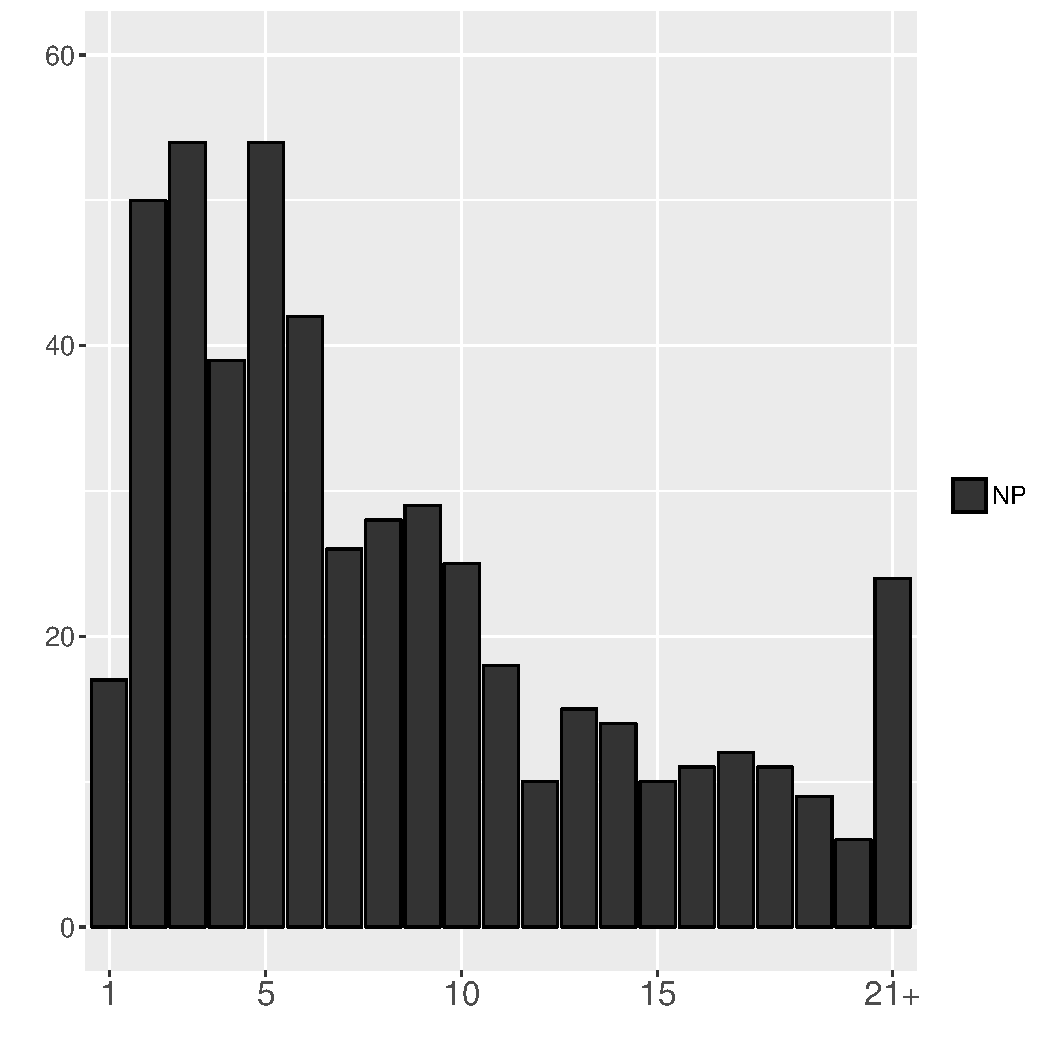
\includegraphics[width=0.6\textwidth]{figure/ExpTypePrevWO.pdf}
	\caption{Antecedent's word order of NPs}
	\label{ExpTypePrevWOF}
	\end{center}
%\end{minipage}
\end{figure}
\begin{figure}
%\begin{minipage}{0.5\textwidth}
	\begin{center}
	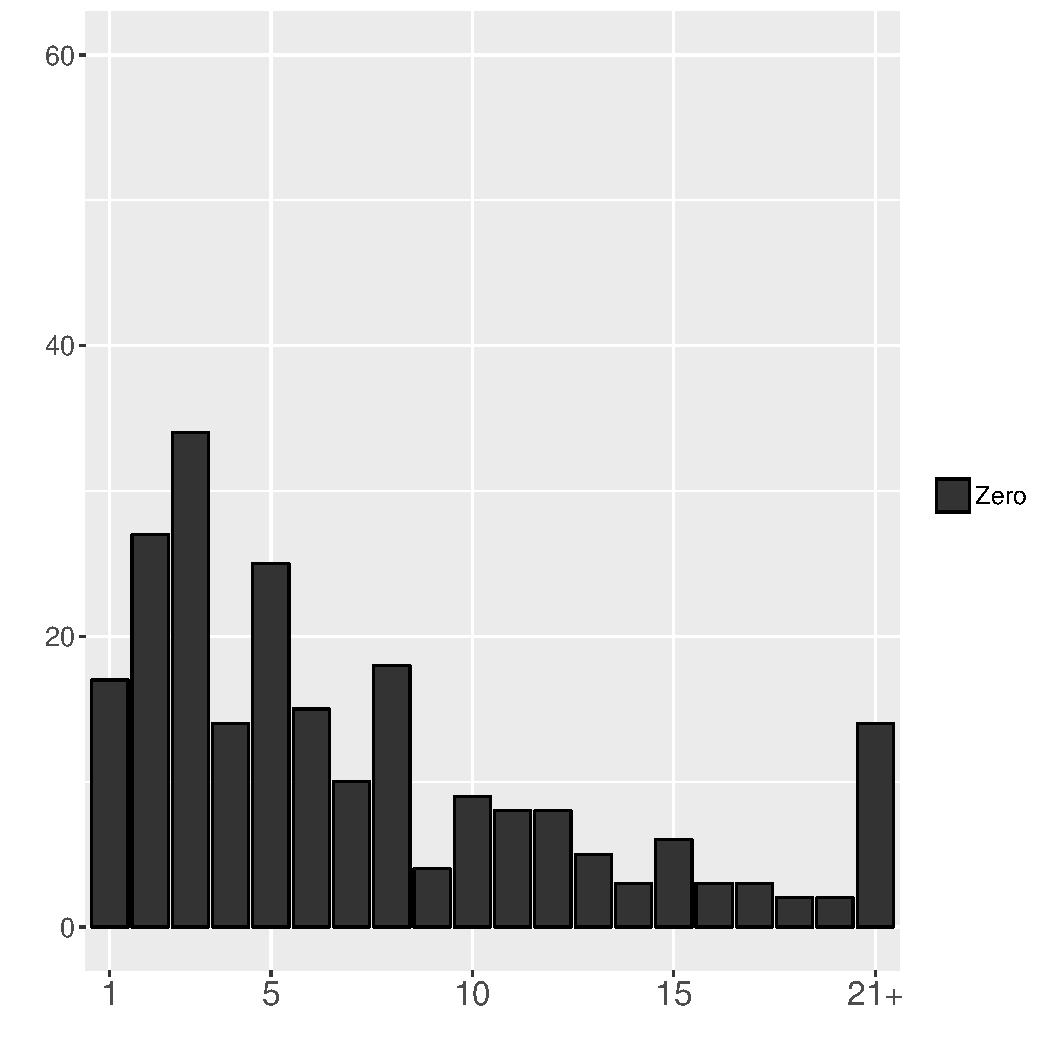
\includegraphics[width=0.6\textwidth]{figure/ExpTypePrevWOZero.pdf}
	\caption{Antecedent's word order of zero pronoun}
	\label{ExpTypePrevWOZeroF}
	\end{center}
%\end{minipage}
\end{figure}

Why are these pronouns or NPs which refer to the immediate antecedent appear (near) clause-initially?
I argue that, in addition to the from-old-to-new principle \ref{oldnewprinciple},
the persistent-element-first principle works in a spontaneous speech.
%
\ex. \label{PerFirstPrinciple}\tl{Persistent-element-first principle}:
 In languages in which word order is relatively free,
 the unmarked word order of constituents is persistent element first and non-persistent element last.

\chd{One of the factors which motivate this principle is  clause-chaining.
In spoken Japanese, a chain of clauses is frequently observed as schematized in \Next,
where the speaker announces the topic at the beginning and continues to talk about it by a chain of multiple clauses.%
 \footnote{
 This is also pointed by Michinori Shimoji (p.c.) on Ryukyuan Languages,
 which belong to the same language family as Japanese.
 }
}
%
\ex.
 \a. \fbox{Topic}
 \b. \fbox{Clause1}
 \b. \fbox{Clause2}
 \b. \fbox{Clause3}
 \b. ...

A specific example of clause-chaining is shown in \Next,
where the topic `Everest Trail' in line a is preannounced,
and the following clauses (b--f) is about this topic `Everest Trail'.
%
\ex.
\ag. \EM{kono} \EM{eberesuto-kaidoo-toiuno-wa} \\
	this Everest-trail-\ab{quot}-\ci{wa} \\
	`{This Everest Trail} is'
\bg. tibetto-to nepaaru-no kooeki-ro-ni-mo nat-te ori-masi-te \\
	Tibet-\ab{com} Nepal-\ab{gen} trade-road-\ab{dat}-also become-and \ab{prog}-\ab{plt}-and \\
	`also used for trading  between Tibet and Nepal.'
\cg. ma zissai-wa nihon-de iu-to \tp{\dvline} \\
	\ab{fl} actual-\ci{wa} Japan-\ab{loc} say-\ab{cond} \\
	`Say, in Japan for example,'
\dg. \EM{\O} takao-san-mitaina yama-miti-nan-desu-keredomo \\
	{\O} Takao-mountain-like mountain-road-\ab{nmlz}-\ab{cop}.\ab{plt}-though \\
	`it's like a road in Mt.\ Takao or something.'
\eg. genti-no hito$\sim$bito-nitotte-wa ee \EM{\O} tuusyoo-ro-to iu-yoona \\
	local-\ab{gen} person$\sim$\ab{pl}-for-\ci{wa} \ab{fl} {\O} trade-road-\ab{quot} say-like \\
\bg. insyoo-no \EM{\O} miti-desi-ta \\
	 impression-\ab{gen} {\O} road-\ab{cop}.\ab{plt}-\ab{past} \\
 `{it} was a road like trading road for local people.'
 \b.[] \hfill{(\code{S01F0151: 105.73-120.14})}
%このエベレスト街道というのは
%チベットとネパールの交易路にもなっておりまして
%ま実際は日本で言うと
%高尾山みたいな山道なんですけれども
%現地の人々にとってはえー通商路というような印象の道でした (S01F0151: 105.73-120.14)

\chd{This pattern is useful because which referent the speaker talks about in the chain of clauses in question.}

%This principle is motivated by processing;
%it is easier for the hearer to process if the topic to be talked about is stated first.
%It is easy also for the speaker to say the topic first
%because s/he has already activated the topic to be talked about,
%but not necessarily how to express the following content.
%	\footnote{
%	This might be the same as the from-old-to-new principle (\ref{oldnewprinciple}).
%	}
Figure \ref{ExpTypePrevWOF} and \ref{ExpTypePrevWOZeroF} show word order of antecedents of NPs and zero pronouns, respectively.
Although the contrast is subtle,
the antecedents of zero pronouns are more skewed to earlier positions than NPs.
%The figure is a bar plot of expression types of elements based on the word orders of their antecedents.
%The x-axis indicates the word order of the antecedents and y-axis indicates the raw frequencies of elements.

Consider the following example \Next.
The speaker mentions the topic `the participants of the trekking' first in line a,
and describes this in the following discourse.
After \Next[f],
the speaker extends the topic and describes each participants.
%
\ex.\label{trekking}
 \ag. e \EM{torekking-sankasya}-nituki-masite-wa \\
 	\ab{fl} trekking-participant-about-\ab{plt}-\ci{wa} \\
	`Concerning the participants of this trekking,'
 \bg. moo hontooni ni-zyuu-go-sai-no ooeru-san-kara \\
 	\ab{fl} really two-ten-five-years.old-\ab{gen} working.woman-\ab{hon}-from \\
	`from 25-year-old working lady,'
 \bg. nana-zyuu-ni-sai-no ozii-san-made \\
 	seven-ten-two-years.old-\ab{gen} old.guy-\ab{hon}-till \\
	`to 72-year-old elderly man,'
 \bg. hizyooni takusan-no hito$\sim$bito-ga \\
 	very many-\ab{gen} person$\sim$\ab{pl}-\ci{ga} \\
	`many people...'
 \b. no, not many people,
 \bg. ta-syu-ni wataru nenree-soo-no hito-ga i-te omosirokat-ta-desu \\
 		many-kind-\ab{dat} cover age-tier-\ab{gen} person-\ci{ga} exist-and interesting-\ab{past}-\ab{plt} \\
		`there were many kinds of people from wide age range and it was interesting.'
		\src{S01F0151: 597.67-610.87}
%S01F0151|00597665L|597.665333|610.870275|L|(F え)トレッキング参加者につきましては(0.192)もう本当に二十五歳の(A オーエル;OL)さんから七十二歳のお爺さんまで(0.278)非常にたくさんの人々が(0.539)(F えー)(0.131)<FV>たくさんのじゃない(0.11)多種に渡る(0.237)年齢層の人がいて面白かったです|[文末]|
%S01F0151|00611451L|611.450993|614.022662|L|で(0.429)みんな人によって趣味が違いまして|/テ節/|
%S01F0151|00614377L|614.37677|626.616677|L|登山から(0.325)(F え)登山が趣味の方もいれば写真を撮るのが趣味の方もいて(0.352)後は(D こせ)高山植物に非常に詳しい方もいれば(0.328)バードウォッチングに詳しくて物凄く立派な双眼鏡を持ってくる方もいたりして|<テ節>|直後がまとめ表現
%S01F0151|00626928L|626.928382|634.442324|L|(F ま)私達はっきり言って何も知らないで参加したので全部人に(0.301)あれは何ですかとか言って聞きながら(0.292)教えていただいて(0.317)登っていました|[文末]|

In this kind of example,
clause-initial elements do not refer to zero pronouns as constituents in the following clauses,
but are only pragmatically associated with the constituents in the following clauses (see also \S \ref{Par:Subj:Ex}).


\begin{table}
 \tblcaption{Antecedent's particle vs.~current expression type}
 \label{ExpTypePrevParT}
\begin{tabular}{lrrrr}
 \toprule
          & \ci{toiuno-wa} & \ci{wa} & \ci{ga} & \ci{o} \\
 \midrule
 NP       & 11             & 38      & 80      & 89 \\
          & \rt{(36.7\%)}  & \rt{(46.3\%)} & \rt{(63.0\%)} & \rt{(74.8\%)} \\
 Pronoun  & 4              & 3       & 5       & 3 \\
          & \rt{(13.3\%)}  & \rt{(3.7\%)} & \rt{(3.9\%)} & \rt{(2.5\%)} \\
 Zero     & 15             & 41      & 42      & 27 \\
          & \rt{(50.0\%)}  & \rt{(50.0\%)} & \rt{(33.1\%)} & \rt{(22.7\%)} \\
 \midrule
 Sum      & 30             & 82      & 127     & 119 \\ 
          & \rt{(100\%)}   & \rt{(100\%)} & \rt{(100\%)} & \rt{(100\%)} \\
 \bottomrule
%           NP Pron Zero
%  toiuno-wa 11    4   15
%  wa        38    3   41
%  ga        80    5   42
%  o         89    3   27
\end{tabular}
\end{table}

\begin{figure}
	\begin{center}
	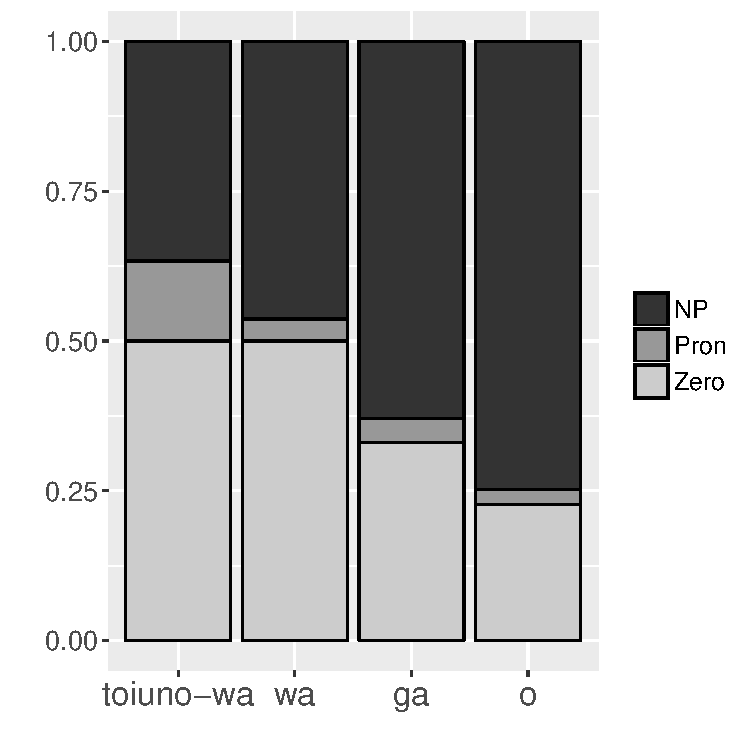
\includegraphics[width=0.5\textwidth]{figure/ExpTypePrevPar.pdf}
	\caption{Antecedent's particle vs.~current expression type}
	\label{ExpTypePrevParF}
	\end{center}
\end{figure}

Not all clause-initial antecedents of zero are coded by topic markers.
Figure \ref{ExpTypePrevParF} is a bar plot of expression types of elements based on the particles of their antecedents.
According to the figure, the antecedents of zero pronouns are more likely to be coded by \ci{wa} or \ci{toiuno-wa} than
those of overt NPs,
although there are many antecedents of zeros coded by \ci{ga} or \ci{o}.

In the following example \Next,
%\ci{syoo-doobutu} `an small animal' in line b is new 
%%
%\ex.
% \a. When we were having dinner,
% \bg. n mado-no tokoro-to iu-ka beranda-ni nanika \EM{syoo-doobutu-ga} koo tyokotyoko-to ki-ta-n-desu-ne \\
% 	\ab{fl} window-\ab{gen} place-\ab{quot} say-\ab{q} balcony-to something small-animal-\ab{nom} this.way \ab{ono}-\ab{quot} come-\ab{past}-\ab{nmlz}-\ab{cop}.\ab{plt}-\ab{fp} \\
%	`a small animal came near the window, or the balcony.'
% \bg. de saisyo koo ano sotira-no soto-no hoo-kara \EM{\O} nozoi-ta mon-desu-kara \\
% 	then at.first this.way \ab{fl} that-\ab{gen} outside-\ab{gen} direction-from {\O} look-\ab{past} thing-\ab{nmlz}.\ab{cop}-because \\
%	`At first, (it) appeared from the outside, that way, so'
% \bg. watasi-wa saisyo \EM{\O} risu-kana-to omot-ta-n-desu \\
% 	\ab{1}\ab{sg}-\ci{wa} at.first {\O} squirrel-\ab{q}-\ab{quot} think-\ab{past}-\ab{nmlz}-\ab{cop}.\ab{plt} \\
%	`at first I thought (it) was a squirrel.'
% \bg. de tu sat-to koo are-to omot-te it-tara sat-to \EM{\O} nige-tyai-masi-te \\
% 	then \ab{frg} \ab{ono}-\ab{quot} this.way \ab{fl}-\ab{quot} think-and go-then \ab{ono}-\ab{quot} {\O} escape-\ab{pfv}-\ab{plt}-and \\
%	`(I) was wondering and approached (the balcony), then (it) ran away.'
%	\src{S00F0014: 612.71-621.50}
%S00F0014|00612711L|612.710582|621.496514|L|それで(0.344)(F あのー)<FV>(0.176)夜に(0.554)(F あの)食事をこうしてましたら(0.748)(F ん)窓のところと言うかベランダに何か小動物がこうちょこちょこと来たんですね|[文末]|
%S00F0014|00621815L|621.814615|627.660077|L|で最初こう(0.282)(F あの)(0.12)そちらの外の方から覗いたもんですから(0.312)私は最初(0.265)リスかなと思ったんです|[文末]|
%S00F0014|00628000L|627.999519|631.707987|L|で(0.329)(D (? つ))さっとこう(F あれ)(0.235)と思って行ったらさっと逃げ(0.169)ちゃいまして|/テ節/|
\ci{waru-gaki} `brats' which is coded by \ci{ga} clause-initially in line a is the antecedent of the zero in line b.
%
\ex.
 \ag. a dokka-no kinzyo-no \EM{waru-gaki-ga} sute-inu-o mi-te \\
		\ab{fl} somewhere-\ab{gen} neighborhood-\ab{gen} bad-brat-\ci{ga} abandon-dog-\ci{o} look-and \\
		`Brats around here found this abandoned dog, and'
 \bg. akai penki-o hana-no ue-ni \EM{\O} nut-ta-n-daroo-to \\
 	red paint-\ci{o} nose-\ab{gen} above-\ab{dat} {\O} paint-\ab{past}-\ab{nmlz}-\ab{infr}-\ab{quot} \\
	`(they) must have painted the dog's nose red.'
 \b. (we) were talking like this.
 \src{S02M0198: 176.26-184.61}
%S02M0198|00176259L|176.258754|184.61063|L|(F あ)どっかの(0.161)近所の悪がきが(0.461)捨て犬を見て(0.599)赤いペンキを(0.263)鼻の上に塗ったんだろうと(0.193)話したんですけども|/並列節ケドモ/|

This might sound a priori to some readers because Japanese is traditionally argued to be an SOV language:
of course \ci{ga}-coded elements are subjects and precede other arguments.
However, what I claim is that
the persistent-element-first principle \ref{PerFirstPrinciple}, in addition to the from-old-to-new principle \ref{oldnewprinciple}, is one of the motivations for so-called subjects (A and S) to precede other arguments.
%As \citeA{lambrecht94} points out, topics tend to be outside of a clause, i.e., they do not belong to the arguments of a clause as in \Next.
%In \Next[a],
%the expression \ci{the African elephant} is not an argument of the predicate \ci{fan};
%\ci{fan} has A as \ci{he} and P as \ci{himself}.
%Similarly, in \Next[b],
%\ci{the typical family today} is also non-argument;
%the argument of the verb \ci{work} is \ci{the husband and the wife}.
%%
%\ex.
% \a. (Six year old girl, explaining why the African elephant has bigger ears than the Asian elephant)
% 	\EM{The African elephant}, it's so hot there, so he can fan himself.
% \b. (From a TV interview about the availability of child care)
% 	That isn't the typical family anymore.
%	\EM{The typical family today}, the husband and the wife both work.
%	\hfill{\cite[][p.~193 (emphasis added)]{lambrecht94}}
%
%In the same way,
%`the participants of the trekking' in (\ref{trekking}) is not an argument of the clause (\ref{trekking}f).
%The argument of the verb \ci{i(ru)} `exist' is \ci{hito} `person'.

Another motivation has been pointed out for topic elements immediately repeated clause-initially.
\citeA{dennakagawa13} discuss cases where clause-initial topics are used as fillers.
Since topics have already been evoked in the speaker's mind, the cost of producing topics is lower than that of producing new elements.
While the speaker utters the topic,
s/he plans the following utterance.
They investigated conversations and found that the topic elements repeated immediately after the previous speaker's utterance
complementarily distribute with fillers.
They also found that the length of the final mora of the topic phrase (typically \ci{wa}) correlates with the length of the following utterance
\cite[see also][]{watanabeden10}.
%This might be another motivation for topics being outside of a clause.
In the following example \Next,
not only `Serbian people' is repeated twice in line a and b,
the whole sentence is almost repeated;
the sentences in line a and b convey almost the same proposition.
This is another piece of evidence that supports their claim;
while repeating almost the same proposition,
the speaker can plan what to say next about this topic.
%
\ex.
 \ag. sono \EM{serubia-zin-no} \EM{kata-tati}-ga soko-ni-wa ma hazimete ee serubia-teekoku-toiu kokka-o tukuru-no-ga maa zyuu-ni-seeki-no ma owari-gurai-nan-desu-ga \\
 	that Serbia-people-\ab{gen} person.\ab{plt}-\ab{pl}-\ci{ga} there-\ab{dat}-\ci{wa} \ab{fl} first.time \ab{fl} Serbia-empire-\ab{quot} nation-\ci{o} make-\ab{nmlz}-\ci{ga} \ab{fl} ten-two-century-\ab{gen} \ab{fl} end-around-\ab{nmlz}-\ab{cop}.\ab{plt}-though \\
	`Thoese Serbian people built a nation called the Serbian Empire towards the end of the eleventh century.'
 \bg. ee kono ziki maa \EM{serubia-no} \EM{kata-tati}-ga maa koko-ni tu kokka-o tukut-te ee serubia-teekoku-toiu koto-de \\
 	\ab{fl} this time \ab{fl} Serbia-\ab{gen} person.\ab{plt}-\ci{ga} \ab{fl} here-\ab{dat} \ab{frg} nation-\ci{o} make-and \ab{fl} Serbia-empire-\ab{quot} thing-\ab{cop}.and \\
	`Around this time Serbian people build a nation, this is Serbian Empire and'
 \bg. ee ryuusee-o \EM{\O} kiwame \\
 		\ab{fl} flourish-\ci{o} {\O} be.extreme \\
	`(it) flourished.'
 \b. At that time from north Catholic was coming, and from south Greek Orthodox was coming,
 \b. though they are both Christian,
 \bg. ee ni-keetoo-no syuukyoo-no naka-de seekatu-o \EM{\O} si-te-iku naka-de \\
 		\ab{fl} two-stream-\ab{gen} religion-\ab{gen} inside-\ab{loc} life-\ci{o} {\O} do-and-go inside-\ab{loc} \\
		`While (they) were living surrounded by two streams of religion,'
 \bg. ee serubia-teekoku-tosite ma dotira-o erabu-ka-tteiu na ko ee koto-no naka-de \\
 	\ab{fl} Serbia-empire-as \ab{fl} which-\ci{o} choose-\ab{q}-\ab{quot} \ab{frg} \ab{frg} \ab{fl} thing-\ab{gen} inside-\ab{cop}.and \\
	`(they) faced a question of which one to choose.'
 \bg. ee ma minami-gawa-no girisya-seekyoo-o \EM{\O} toru wake-nan-desu-ga \\
 	\ab{fl} \ab{fl} south-side-\ab{gen} Greek-Orthodox-\ci{o} {\O} choose reason-\ab{nmlz}-\ab{cop}.\ab{plt}-though \\
	`(They) eventually chose Greek Orthodox.'
	\src{S00M0199: 212.34-221.02}
%S00M0199|00212336L|212.336343|221.023973|L|そのセルビア人の方達がそこには(F ま)初めて(0.163)(F えー)セルビア帝国という(0.373)(F えー)国家を作るのが(F まー)十二世紀の(0.436)(F ま)終わりぐらいなんですが|/並列節ガ/|
%S00M0199|00221455L|221.455248|229.24769|L|(F えー)この時期(F まー)(0.976)セルビアの方達が(F まー)ここに(D つ)国家を作って(0.151)(F えー)セルビア帝国ということで(0.266)(F えー)隆盛を極め|/連用節/|
%S00M0199|00229652L|229.651772|254.15569|L|(F えー)そしてその後(F まー)(F あのー)(F まー)その当時宗教としては(0.337)(F えー)北からは(F えー)(0.13)(D く)(F ま)キリスト教のカトリック(0.128)(F えー)南からは(0.372)(F えー)(F い)ギリシャ正教ということで(F えー)二つの(F えー)(F ま)同じキリスト教ですが(F えー)二系統の宗教の中で(0.327)生活をしていく中で(0.391)(F えー)セルビア(0.177)帝国として(F ま)どちらを選ぶかっていうな(0.212)(D こ)(F えー)ことの(D ん)中で(F えー)(0.14)(F ま)(0.561)南側のギリシャ正教を取る訳なんですが|/並列節ガ/|


%%----------------------------------------------------
\subsection{Summary of clause-initial elements}

This section investigated characteristics of clause-initial elements.
It turned out that
shared and persistent elements tend to appear clause-initially.
Not only this study confirmed the classic observation that
topics tend to appear clause-initially,
this section and the next section analyze what kind of topics appear clause-initially.
I also discussed motivations for clause-initial topics.


%%----------------------------------------------------
%%----------------------------------------------------
\section{Post-predicate elements}\label{WOPostPreEles}

While Japanese is reported to be a verb-final language \cite{hinds86,shibatani90},
some elements appear after the verb in spoken Japanese \cite{kuno78,onosuzuki92,fujii95,takami95a,takami95b,ono06,nakagawaetal08_paper}.
The following are examples of post-predicate elements.
Since post-predicate elements are very rare in monologues,
the examples are from the dialogue part of CSJ.
\ci{Kono hito} `this person' in \Next and \ci{terii itoo} `Terry Ito (A person's name)' in \NNext are produced after the predicates \ci{yat} `do' and \ci{kake} `wear', respectively.
%
\ex.
\ag.[R:] nani \EMi{yat}-teru-no \EM{kono} \EM{hito} \\
 		what do-\ab{prog}-\ab{nmlz} this person \\
		`What is (he) doing, this person?'
		\src{D02F0028: 193.30-194.45}

\ex.\label{D02F0015_TerryIto}
 \ag.[L:] sangurasu-toka \EMi{kake}-te-masu-yo-ne \EM{terii} \EM{itoo-tte} \\
		sunglasses-\ab{hdg} wear-\ab{prog}-\ab{plt}-\ab{fp}-\ab{fp} Terry Ito-\ab{quot} \\
		`(He) is wearing sunglasses, isn't he, Terry Ito?'
		\src{D02F0015: 359.17-362.42}

This section investigates the information structure of post-predicate construction of this kind.
Although post-predicate expressions could be adverbs, connectives, and other adjuncts,
this study only examine noun phrases.
%I call all the elements which appear before the predicate
%``elements before the predicate'' or ``preposed elements''
%as opposed to ``post-predicate'' or ``postposed'' elements.
%I keep the term ``pre-posed'' elements
%to indicate elements which appear immediately before the predicate
%(to be discussed in \S \ref{WOPrePredEles}).

%%----------------------------------------------------
\subsection{Strongly evoked elements appear after predicate}\label{WORdis}

\citeA[][p.~136]{takami95a} argues that
postposed elements are elements other than focus.
For example,
the answer to a question or \ci{wh}-phrase cannot be postposed naturally.
\Next is an example of a postposed element `a 10-carat diamond ring' as the answer to the question `what'.
While the sentence itself is natural,
the postposed element cannot felicitously be the answer to a question.
%
\ex.
 \a.[Q:] What did Taro buy for Hanako?
 \bg.[A:] \#taroo-wa hanako-ni kat-te yat-ta-yo \EM{zyuk-karatto-no} \EM{daiya-no} \EM{yubiwa-o} \\
 		Taro-\ci{wa} Hanako-for buy-and give-\ab{past}-\ab{fp} 10-carat-\ab{gen} diamond-\ab{gen} ring-\ci{o} \\
		`Taro bought (it) for Hanako, a 10-carat diamond ring.'

Similarly,
\ci{wh}-phrases such as \ci{dore} `which' cannot be postposed
as shown in \Next.
%
\exg. *itiban oisii-desu-ka \EM{dore-ga}? \\
		most delicious-\ab{cop}.\ab{plt}-\ab{q} which-\ci{ga} \\
		`The most delicious one, which?'


%As has been pointed out in \citeA{onosuzuki92,takami95b,ono06,nakagawaetal08_paper},
%topics can be postposed.
\citeA{nakagawaetal08_paper} found that
there are two types of post-predicate construction:
single-contour type and double-contour type.
The single-contour type is a type of post-predicate construction
where the post-predicate elements are uttered without a pause and does not have the F$_{0}$ peak,
whereas the double-contour type is a type of construction
where the post-predicate elements are uttered with a pause and does have the F$_{0}$ peak.
The pitch contours of each utterance is shown in Figure \ref{kome1F} for single-contour type (\Next[A] and \NNext[A]) and \ref{kome2F} for double-contour type (\Next[A$^{\prime}$] and \NNext[A$^{\prime}$]),
both of which are produced by the author.
The post-predicate part is \ci{kome-wa} `rice-\ci{wa}',
whose accent nucleus is on \ci{me} and overall accent is supposed to be LHL (L indicates low and H indicates high in pitch).
In Figure \ref{kome1F}, where the postposed element is uttered in the same continuous contour as the main clause,
one cannot observe the F$_{0}$ peak in \ci{me} nor a pause between the predicate and the postposed element.
In Figure \ref{kome2F}, on the other hand,
where the postposed element is uttered in a separate contour from the main clause,
one can observe the F$_{0}$ peak in \ci{me} and a pause between the predicate and the postposed element.

Nakagawa et al. investigated the difference between these two types in terms of information structure and found that
the post-predicate elements of the single-contour type are evoked
by being mentioned immediately before or through physical context.
On the other hand,
those of the double-contour type are not necessarily evoked.
For example, compare the following examples \Next and \NNext,
where the bold-faced letters indicate that
they are high in pitch.%
	\footnote{
	Here I assume that the pitch accent of \ci{oisii} `good' is LHHH
	and that of \ci{kome-wa} `rice-\ci{wa}' is LHL.
	}
The referent `rice' in \Next is evoked
because it is mentioned in \Next[Q] immediately before the answer to Q is uttered.
In this case,
\Next[A$^{\prime}$],
where the post-predicate element \ci{kome-wa} `rice-\ci{wa}' has its own F$_{0}$ peak and is preceded by a pause,
is not acceptable,
while \Next[A],
where the post-predicate element without its own F$_{0}$ peak is uttered immediately after the predicate without a pause,
is acceptable.
%
\ex. \tl{The referent `rice' evoked}
 \a.[Q:] I don't like rice.
	\bg.[A:] o\pk{isii}-yo \ul{kome-wa} \\
			good-\ab{fp} rice-\ci{wa} \\
	\bg.[A$^{\prime}$:] ?o\pk{isii}-yo, \ul{ko\pk{me}-wa} \\
			good-\ab{fp} rice-\ci{wa} \\
			`RICE is good (but others not).'
			\hfill{\cite[][p.~7]{nakagawaetal08_paper}}

On the other hand,
in \Next, where `rice' is not evoked before the speaker utters \Next[A] or \Next[A$^{\prime}$],
only double-contour type \Next[A$^{\prime}$] is acceptable
and the single-contour type \Next[A] is not natural.
\ex. \tl{The referent `rice' not evoked}
 \a.[Q:] Is that sushi bar good?
	\bg.[A:] ??o\pk{isii}-yo \ul{kome-wa} \\
			good-\ab{fp} rice-\ci{wa} \\
	\bg.[A$^{\prime}$:] o\pk{isii}-yo, \ul{ko\pk{me}-wa} \\
			good-\ab{fp} rice-\ci{wa} \\
			`RICE is good (but others not).'
			\hfill{(ibid.)}

The remaining issue is
to investigate the difference between elements before and after the predicate in terms of information structure.

\begin{figure}
%\begin{minipage}{0.5\textwidth}
	\begin{center}
	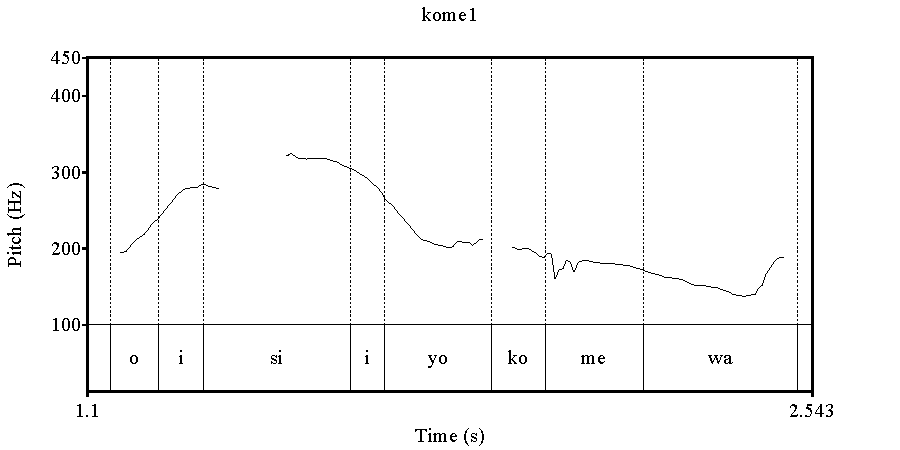
\includegraphics[width=0.6\textwidth]{sounds/kome1.pdf}
	\caption{Post-predicate construction: single-contour type}
	\label{kome1F}
	\end{center}
%\end{minipage}
\end{figure}
\begin{figure}
%\begin{minipage}{0.5\textwidth}
	\begin{center}
	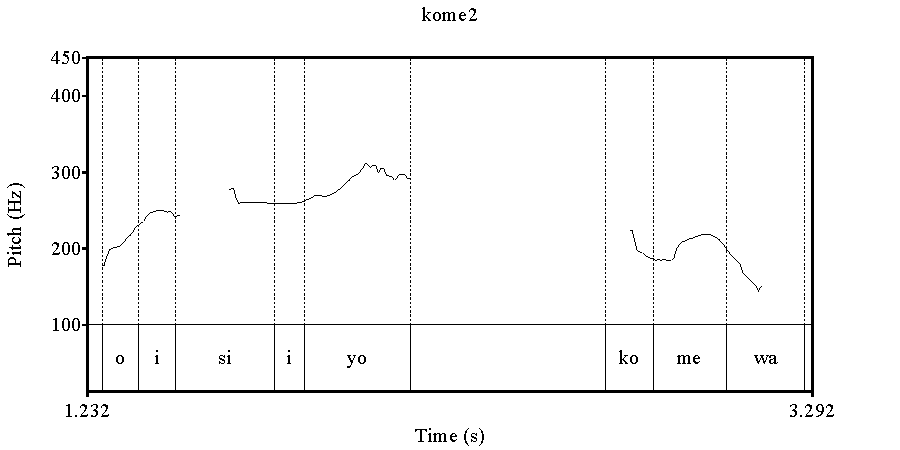
\includegraphics[width=0.6\textwidth]{sounds/kome2.pdf}
	\caption{Post-predicate construction: double-contour type}
	\label{kome2F}
	\end{center}
%\end{minipage}
\end{figure}

\citeA{nakagawaetal08_paper} measured the referential distance (RD) between the post-predicate elements and their antecedents,
i.e., they measured the number of inter-pausal units between the element in question and its antecedent.
They modified the definition of RD from the original one \cite{givon83} and decided to use inter-pausal unit as a measure of RD
since clause boundaries are sometimes difficult to identify in spoken Japanese.
Their results are shown in Table \ref{RDPostT}.
The table shows that the average RD of the post-predicate elements of single-contour type is 6.9 on average,
whereas that of double-contour type is 39.7.
What about elements before the predicate?

I conducted the same investigation for elements before the predicate, but this time I used monologues employed throughout this dissertation
because the dialogues they used in their study lack the information about RD of elements before the predicate.%
	\footnote{
	Nakagawa et al. counted the RD of non-anaphoric elements as 100 (the maximum value of RD),
	but this study didn't include non-anaphoric elements
	since I thought that this is too arbitrary.
	This modification makes the RD of elements before the predicate (conducted in this study) smaller.
	This has only a small effect and the overall conclusion does not change because,
	according to our result,
	the RD of pre-predicate elements are larger than that of post-predicate elements;
	If this study employed the same criteria as Nakagawa et al.,
	the RD of elements before the predicate are expected to be even larger.
	}
Further study is needed to make sure that elements before the predicate in monologues and dialogues have the same characteristics.
Table \ref{RDPreT} shows the average RDs of elements before the predicate based on their word order.
Here, I simplified word order to only include arguments in the count (excluding fillers, fragments, adverbs, adjectives, etc.).
\code{1} indicates that the element in question is the first argument in a clause,
\ci{2} indicates that it is the second argument, and so on.
The RD of the first argument is 20.9 on average,
that of the second argument is 23.0, and
the third is 41.1.
%the fourth is 70.5.
The table indicates that the RDs of elements before the predicate,
regardless of their word orders,
are larger than that of postposed elements of the single-contour type.
The RD of double-contour postposed elements is similar to that of preposed elements in the third position.
I do not have explanation for the RD of double-contour postposed elements.
I believe that postposed elements of the double-contour type are heterogeneous;
some might be afterthought,
some might have interactional functions \cite{ono07},
others might be something else (\citeA{tanaka05,kakuden12}, see also the discussion in \S \ref{WO:PostP:Motiv:Double}).
What I want to emphasize here is that the RD of the single-contour postposed elements is smaller than elements before the predicate.
The postposed elements of the single-contour type are evoked when they are uttered;
their activation cost is low.
Taking into consideration the fact that
many of the post-predicative elements are pronouns or nouns preceded by demonstratives \cite{nakagawaetal08_paper},
I propose that post-predicative elements are often strongly evoked.
On the other hand, the activation cost of preposed elements is higher than that of postposed elements.%
 \footnote{
 The average RD of zero pronouns is 5.0,
 which shows that post-predicate elements of single-contour type is
 close to zero pronouns.
 }

\begin{table}
%\begin{minipage}{0.5\textwidth}
 \centering
 \caption{RD of post-predicate elements}
 \begin{tabular}{lrr}
 \toprule
   & Single-contour & Double-contour \\
 \midrule
  RD & 6.9 & 39.7 \\
 \bottomrule
 \end{tabular}
 \label{RDPostT}
% \end{minipage}
\end{table}
\begin{table}
% \begin{minipage}{0.5\textwidth}
  \centering
 \caption{RD of elements before predicate}
 \begin{tabular}{lrrrr}
 \toprule
  &  1  & 2 & 3 \\
 \midrule
 RD & 20.9 & 23.0 & 41.1 \\
 \bottomrule
 \end{tabular}
 \label{RDPreT}
% \end{minipage}
\end{table}

The following are examples of post-predicate constructions from dialogues.
\Next and \NNext are examples of single-contour type.
The postposed elements of this type are typically pronouns or modified by demonstratives such as \ci{kono} `\ab{dem}.\ab{prox} (this)', \ci{sono} `\ab{dem}.\ab{med} (this/that)', \ci{ano} `\ab{dem}.\ab{dist} (that)'.
In \Next,
the postposed element is the pronoun \ci{kore} `\ab{dem}.\ab{prox} (this)'.
The participants are working on a tasks of ranking famous people based on how much they earn.
The utterance is produced in the middle of this tasks and
the demonstrative \ci{kore} refers to the ranking so far.
Therefore, the referent of \ci{kore} is expected to be evoked in the participants' mind.
As shown in Figure \ref{D02F0025_sugoi_tatakaiF},
where the upper box indicates the intensity of the utterance
and the under box indicates the F$_{0}$,
the postposed element \ci{kore} does not have F$_{0}$ peak.
%
\ex. \label{D02F0025_sugoi_tatakai}
	\ag.[L:] sugoi tatakai-da-yo-ne \EM{kore} \\
	awful battle-\ab{cop}-\ab{fp}-\ab{fp} this \\
	`(It) is an awful battle, this?'
		\src{D02F0025: 463.93-465.81}

In \Next,
where the participants are involved in the same task as \Last,
\ci{kono hito} `this person' is the famous person under discussion right now and hence the referent is evoked in the participants' mind.
Figure \ref{D02M0028_konohitoF} shows the intensity and the F$_{0}$ of the utterance \Next.
Although the F$_{0}$ of the postposed element is not shown because the speaker's utterance is too quiet,
the intensity tells us that
the postposed part is uttered without a pause.
Also, the fact that the intensity is low indicates that the postposed element is only weakly uttered because the referent is evoked enough.
%
\ex.\label{D02M0028_konohito}
	\ag.[R:] nani yat-teru-no \EM{kono} \EM{hito} \\
			what do-\ab{prog}-\ab{nmlz} this person \\
			`What is (he) doing, this person?'
		\src{D02M0028: 193.30-194.45}

Common nouns can also be postposed elements of the single-contour type as in \Next.
In \Next, where the participants are again involved in the same task,
the postposed element \ci{syasin} `photo' is uttered without a pause or F$_{0}$ peak as shown in Figure \ref{D02F0015_syasinF}.
Since R, the other participant, has photos physically and this is part of their rules of the task,
it is reasonable to assume that the participants have already evoked photos.
%
\ex.\label{D02F0015_syasin}
	\ag.[L:] siro-kuro-desu-ka \EM{syasin} \\
		white-black-\ab{cop}.\ab{plt}-\ab{q} photo \\
		`Are (they) black-and-white, the photo?'
		\src{D02F0015: 313.95-315.26}

\begin{figure}
%\begin{minipage}{0.5\textwidth}
	\begin{center}
	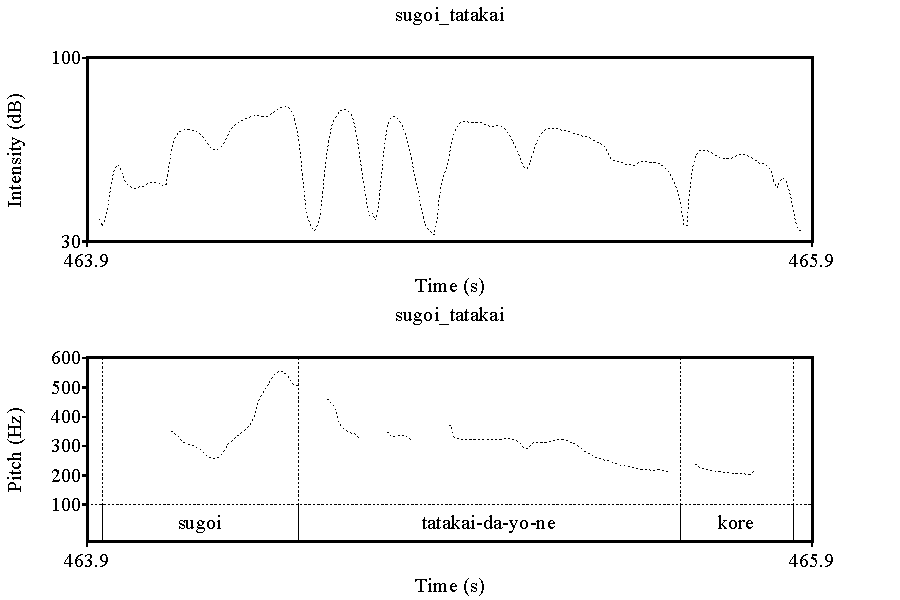
\includegraphics[width=0.6\textwidth]{sounds/D02F0025_sugoi_tatakai.pdf}
	\caption{Intensity and F$_{0}$ of single-contour type \ref{D02F0025_sugoi_tatakai}}
	\label{D02F0025_sugoi_tatakaiF}
	\end{center}
%\end{minipage}
\end{figure}
\begin{figure}
%\begin{minipage}{0.5\textwidth}
	\begin{center}
	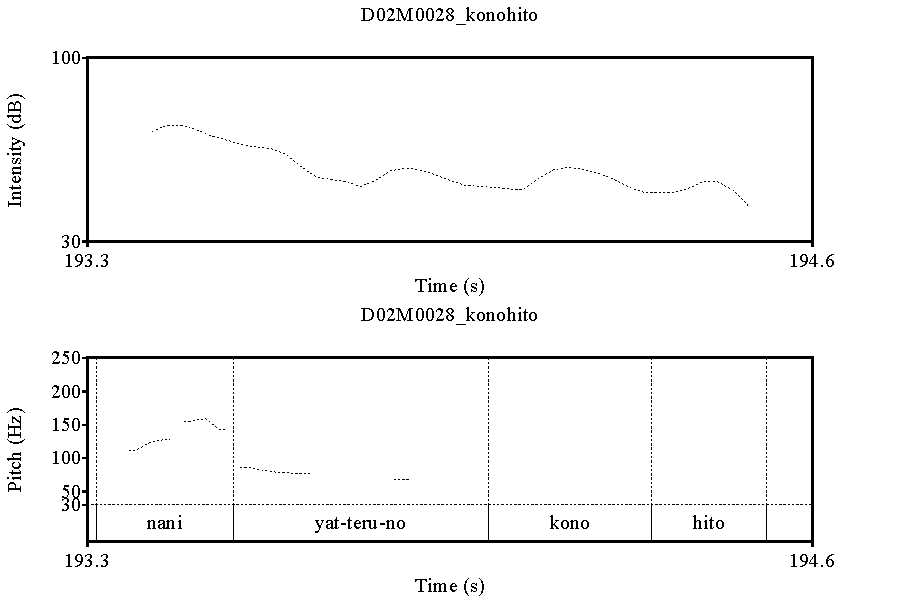
\includegraphics[width=0.6\textwidth]{sounds/D02M0028_konohito.pdf}
	\caption{Intensity and F$_{0}$ of single-contour type \ref{D02M0028_konohito}}
	\label{D02M0028_konohitoF}
	\end{center}
%\end{minipage}
\end{figure}
\begin{figure}
%\begin{minipage}{0.5\textwidth}
	\begin{center}
	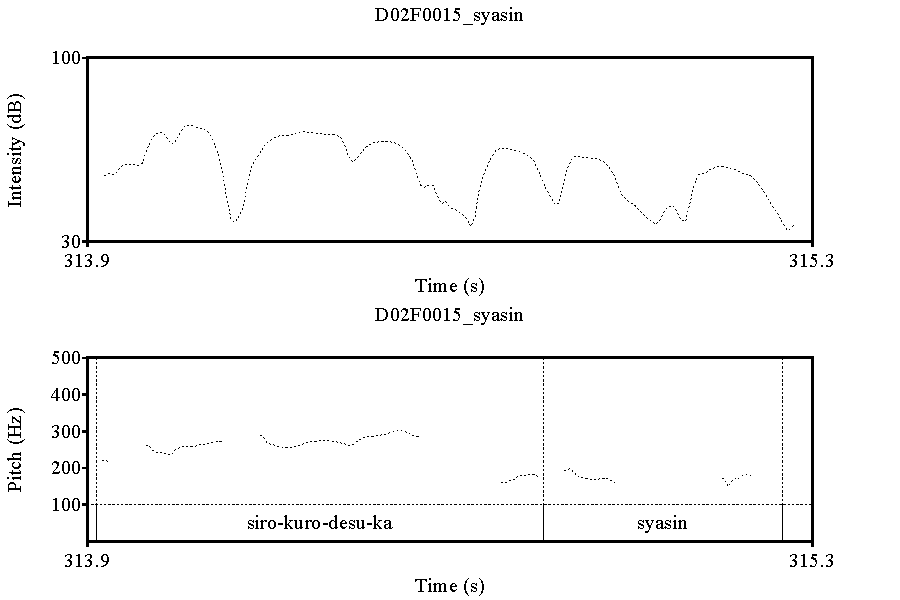
\includegraphics[width=0.6\textwidth]{sounds/D02F0015_syasin.pdf}
	\caption{Intensity and F$_{0}$ of single-contour type \ref{D02F0015_syasin}}
	\label{D02F0015_syasinF}
	\end{center}
%\end{minipage}
\end{figure}


On the other hand,
postposed elements of the double-contour type have not been evoked enough or they are contrastive at the time of utterance.
In \Next, where again the participants are involved in the task of ranking famous people based on their income,
\ci{kotti-wa} `on my side' is uttered in a separate contour from the main clause and there is a pause between the main clause and the postposed element as shown in Figure \ref{D02F0015_kottiwaF}.
`On my side' is necessary information in the sense that
the other participant L was talking about how many people were listed on her own side.
Therefore, the participant R might have thought that `there are ten people' is not enough and add `on my side' later.
The F$_{0}$ peak of the postposed \ci{kotti-wa} `on my side' is still lower than \ci{zyuu} `ten' in the main clause,
and the intensity is also lower.
This is because the postposed element is not focus as \citeA{takami95a,takami95b} has pointed out.
Foci are typically new in the given-new taxonomy and need F$_{0}$ peak and intensity in order for the hearer to understand clearly what is said.
%
\ex.\label{D02F0015_kottiwa}
 \a.[L:] There are eleven people (listed on my side).
 \bg.[R:] zyuu-nin-desu \EM{kotti-wa} \\
 		ten-people-\ab{cop}.\ab{plt} this.side-\ci{wa} \\
		`There are ten people on my side.'
	\src{D02F0015: 3.27-9.03}

%Similarly in \Next,
%where the participants are involved in the same task,
%the participants were talking about how the compensation system works in the show business and .
%%
%\ex.\label{D02F0015_geenookai}
% \ag.[L:] kore-wa dan-zyo-no sa-wa nai-n-desu-ka-ne geenookai-tte \\
% 		this-\ci{wa} male-female-\ab{gen} difference-\ci{wa} not.exist-\ab{nmlz}-\ab{cop}.\ab{plt}-\ab{q}-\ab{fp} show.business-\ab{top} \\
%		`Isn't there difference between men and women (income), the show business?'
%	\src{D02F0015: 890.51-893.82}

In \Next,
L is interviewing about R's study on the difference among Japanese dialects.
R utters `western area' in a separate contour from the predicate
because R compares different dialects and, only in eastern area, she didn't find any differences among smaller areas (prefectures).
Therefore `the eastern area' is contrasted with other areas.
In this case, the F$_{0}$ peak and the intensity of the postposed element are as high as those of the main clause
as shown in Figure \ref{D04F0050_kantooF}.
%
\ex.\label{D04F0050_kantoo}
 \ag.[R:] kooiu sa-ga aru-ne-tte iu-koto-wa ie-nai zyootai-desi-ta-ne \EM{kantoo-no} \EM{hoo-wa} \\
 	such.and.such difference-\ci{ga} exist-\ab{fp}-\ab{q} say-thing-\ci{wa} say-\ab{neg} situation-\ab{cop}.\ab{plt}-\ab{past}-\ab{fp} east-\ab{gen} direction-\ci{wa} \\
	`One cannot say that there is such as such difference, eastern area.'
	\src{D04F0050: 338.54-349.27}

\begin{figure}
%\begin{minipage}{0.5\textwidth}
	\begin{center}
	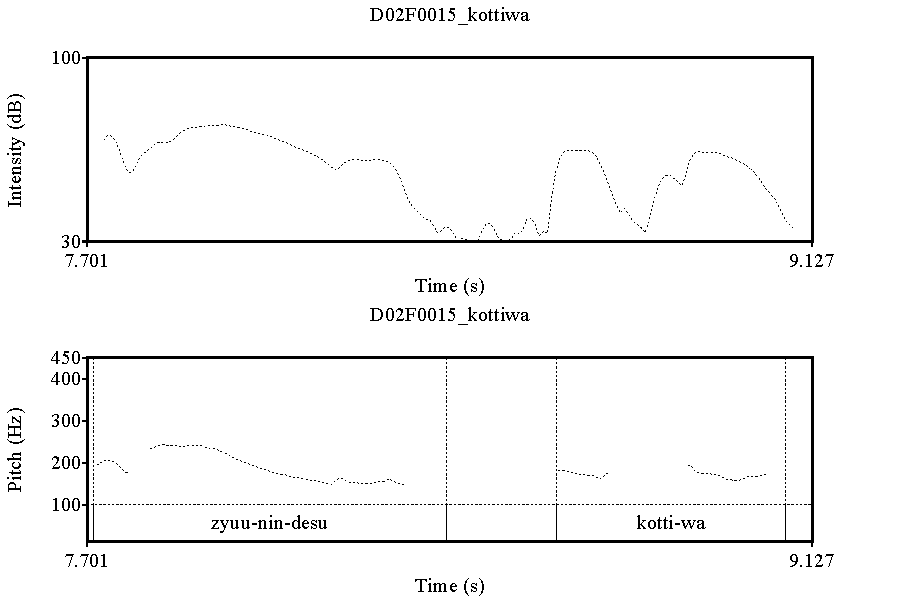
\includegraphics[width=0.6\textwidth]{sounds/D02F0015_kottiwa.pdf}
	\caption{Intensity and F$_{0}$ of double-contour type \ref{D02F0015_kottiwa}}
	\label{D02F0015_kottiwaF}
	\end{center}
%\end{minipage}
\end{figure}
\begin{figure}
%\begin{minipage}{0.5\textwidth}
	\begin{center}
	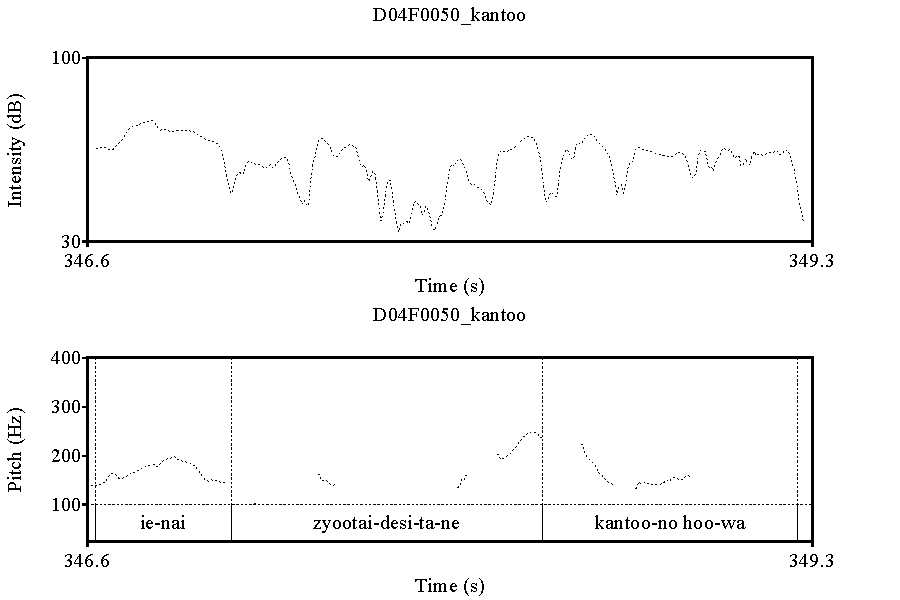
\includegraphics[width=0.6\textwidth]{sounds/D04F0050_kantoo.pdf}
	\caption{Intensity and F$_{0}$ of double-contour type \ref{D04F0050_kantoo}}
	\label{D04F0050_kantooF}
	\end{center}
%\end{minipage}
\end{figure}



%%----------------------------------------------------
\subsection{Motivations for topics to appear post-predicatively}\label{WO:PostP:Motivations}

It has been pointed out that
topics or given elements tend to appear clause initially \cite{mathesius28,firbas64,danes70}.
Then, what are motivations for them to appear post-predicatively?
In this section I mainly discuss the post-predicate elements of single-contour type in comparison with the elements before the predicate.
Those of double-contour type is heterogeneous as discussed above and this needs further investigation.


%%----------------------------------------------------
\subsubsection{Low activation cost and general characteristics of intonation unit}\label{WO:PostP:Motivations:IU}

Before getting directly into the question of
why some topics appear post-predicatively,
let us begin with the question of why some topics do not appear clause-initially.
As discussed in \S \ref{GivenAppearClause-Initially} and this section,
the activation cost of preposed topics is higher than
those of postposed topics and zero pronouns.
The low activation cost of post-predicate elements suggests that
they are not anchors to the previous discourse;
since they are already evoked enough,
they do not have to relate the previous contexts and the current utterance.
Therefore, they have at least motivations for not appearing clause-initially.
Why do they appear post-predicatively?

I argue that the element whose activation cost is low tend to appear post-predicatively
because, in Japanese and many other languages,
an intonation unit starts from high F$_{0}$ and gradually declines toward the end 
\cite{libermanpierrehumbert84,cruttenden86,duboisetal93,chafe94,prieto96,truckenbrodt04,denetal10}.
Since the elements with low activation cost does not require high F$_{0}$,
their preferred position is toward the last position in an intonation unit.
This kind of phenomenon has been already reported in Siouan, Caddoan, and Iroquoian languages of North America \cite{mithun95}.
In these languages,
this newsworthy-first (i.e., given-last) word order is fully grammaticalized, and Mithun proposes a hypothesis that the given-last word order comes from right-detachment constructions, namely, the postposed constructions discussed in this section.
She argues that this word order is motivated by the general tendency that intonation units start from high F$_{0}$, which gradually declines.
This tendency of intonation units is physiologically motivated,
as \citeA{cruttenden86} discusses:
%
\begin{quote}
The explanation for declination has often been related to the decline in transglottal pressure as the speaker uses up the breath in his lungs.
A more recent explanation suggests that an upward change of pitch involves a physical adjustment which is more difficult than a downward change of pitch,
the evidence being that a rise takes longer to achieve than a fall of a similar interval in fundamental frequency.
\cite[][p.~168]{cruttenden86}
\end{quote}
%

Moreover, \citeA[][p.~89]{comrie89} argues that unstressed constituents such as clitic pronouns are cross-linguistically ``subject to special positioning rules only loosely, if at all, relating to their grammatical relation'';
therefore, he argues that ``sentences with pronouns can be discounted in favour of those with full noun phrases''.
%I believe that this tendency is also the case not only with pronouns but also given full NPs in Japanese
%because, in Japanese, pronouns are not very frequent and full NPs are frequently used to refer to activated referent and they are frequently unstressed \cite[\S 6.3]{venditti00}.
Arguing against the hypothesis \cite{givon79}
that one can reconstruct ancient word order of a language based on pronominal affixes and clitics,
Comrie suggests that the order of pronominal affixes and clitics in a clause is more likely to be influenced by stress rhythm properties \cite[][p.~218]{comrie89}.

I argue that the order of Japanese unstressed pronouns and NPs are also affected by some phonetic constraints as Comrie suggests.
As will be discussed in Chapter \ref{Intonation},
some unstressed pronouns and NPs referring to highly evoked entities
lose pitch peaks and are produced only in low pitch.
However, an accent rule in Japanese does not allow lexical items to start with two low pitch morae in a row.
Therefore, the best position for unstressed items is the sentence-final or post-predicate position,
which allows unstressed items to appear.
For phonetic analysis of unstressed items,
see Chapter \ref{Intonation}.


%%----------------------------------------------------
\subsubsection{Why post-predicate construction mainly appears in dialogue and the source of ``emotive'' usage}

The declination of F$_{0}$ does not fully explain post-predicate constructions in Japanese.
The discussion above does not explain why Japanese post-predicate construction mainly appears in dialogues, but not in monologues.
Moreover, Japanese post-predicate constructions are reported to have ``emotive'' characteristics \cite{ono07}.
As examples for emotive characteristics of post-predicate constructions, consider the following constructed example.
Let us assume that a boy gave a present to his girlfriend.
The girl happily received the gift and opened it.
After seeing the gift, say a banana case,%
	\footnote{
	Bananas of all sizes can fit into this banana case.
	}
she uttered \Next or \NNext.
Since the most frequent word order in Japanese is predicate-final,
the canonical order is \Next and
\NNext can be regarded as a post-predicate construction.
%
\exg.\label{korenani}kore nani \\
	this what \\
	`What's this?'
	\hfill{(Canonical word order)}

\exg.\label{nanikore}nani kore \\
	what this \\
	`What's this (weird thing)?'
	\hfill{(Post-predicate construction)}

These two utterances consist of the same constituents \ci{kore} `this' and \ci{nani} `what'.
As has been pointed out in \citeA{onosuzuki92} and \citeA{ono07},
however, the implicatures of these two are different.
In \LLast,
she simply does not know what she received,
probably because she has never seen it before.
Contrastively, in \Last,
she knows what she received (it's a banana case) but she did not like it, as we expected.
\chd{In other contexts, \Last can be used to express the speaker's surprise,
excitement, etc.
However, \Last can never be a neutral question.}
Where does this implicature come from?

Since these two utterances consist of exactly the same elements,
it is obvious that the implicature in \Last cannot be derived from the meaning of each constituent.
In this study, I propose two factors involved in the questions of why post-predicate constructions mainly appear in dialogues and of what the source of this ``emotive'' usage is:
word order and intonation.

Firstly, I concentrate on the relation between word order and why they appear mainly in dialogues.
My point is that,
since the intonation-unit-final position is a position for expressions with interactional functions,
the post-predicate element (of the single-contour type) plays some interactional role.
As has traditionally been argued \cite[e.g.,][]{watanabe71},
the post-predicate position is for interaction in Japanese.
\citeA{iwasaki93} extended this argument and claimed that
in fact the intonation-unit-final position is the position for interaction;
the post-predicate position is only one of examples of this intonation-unit-final position.
Consider the following example.
Each line corresponds to a single intonation unit.
The lines a, b, and c end with interactional markers \ci{ne} and \ci{sa},
which is indicated by \EM{IT}.%
As examples \Next show,
these interactional markers appear IU-finally.
	\footnote{
	IT stands for ``interactional component'',
	one of four types of components in an intonation unit.
	Other types are:
	LD (lead component (e.g., fillers)),
	ID (ideational component), and
%	SU (subjective component), and
	CO (cohesive component).
	The order of an intonation unit is proposed to be
	LD ID CO IT in Japanese \cite[][p.~44]{iwasaki93}.
	}
%
\ex.
 \a.
 \glll sooiu sito-ga siki si-te-\EM{ne} \\
 	such person-\ci{ga} lead do-and-\ab{fp} \\
	ID ID ID ID-CO-\EM{IT}	 \\
	\glt `Such people led, and'
 \b.
 \glll sinin-o asoko-e minna-\EM{ne} \\
 		corpses-\ci{o} there-\ab{dir} all-\ab{fp} \\
		ID ID ID-\EM{IT} \\
%	\glt `'
 \b.
 \glll ano dote-no ue-e-\EM{sa} \\
 		that bank-\ab{gen} top-\ab{dir}-\ab{fp} \\
		ID ID ID-ID-\EM{IT} \\
%	 \glt `'
 \glll atsume-te \\
 		gather-and \\
		ID-CO \\
	\glt `gathered dead bodies on top of that bank...'
	\hfill{\cite[][p.~47, gloss and transcription modified by the current author]{iwasaki93}}

As \citeA{morita05} suggests,
a general function of interactional particles such as \ci{ne} and \ci{sa} is ``to foreground a certain stretch of talk as an `interactionally relevant unit' to be operated on
-- whether that unit is itself a whole utterance or merely one particular component of that utterance'' (p.~92).
Since the post-predicate elements follows these interactional particles within the same intonation unit as in \ref{D02F0015_TerryIto} and \ref{D02F0025_sugoi_tatakai},
where the post-predicate elements follow \ci{ne},
they are also expected to have some interactional functions.
\citeA{kakuden12} report that
77.6\% of the post-predicate constructions have interactional particles of this kind after the predicate,
whereas only 47.0 \% of the non-post-predicate constructions have interactional particles.
This also suggests that post-predicate constructions are related to
some interactional characteristics.
Further investigation is necessary for the question of what kind of interactional functions they have,
possibly employing conversational analysis.

Secondly,
I argue that 
the source of ``emotive'' implicature of \ref{nanikore} in contrast with \ref{korenani} comes from the intonational constraint of the post-predicate element.
In Japanese, \ci{wh}-questions can be optionally uttered in rising intonation.
%%% 要文献
However, the post-predicate element is always falling and the rising intonation is not natural.
Figure \ref{nanikoreF} shows the pitch contour of the utterance \ci{nani kore} `what's this (weird thing)?' \ref{nanikore},
while Figure \ref{korenaniF} shows the pitch contour of neutral order \ci{kore nani} `what's this?' \ref{korenani}.
As indicated in the figures, the neutral word order \ref{korenani} in Figure \ref{korenaniF} is uttered in rising intonation,
and I believe that this is the most frequent intonation,
whereas the post-predicate construction \ref{nanikore} in Figure \ref{nanikoreF} is falling intonation,
in which case it is impossible to utter \ci{kore} with rising intonation.
%Questions with falling intonation convey negative emotion of the speaker.
It is this constraint on the intonation of post-predicate elements to cause emotive implicature of the utterance \ref{nanikore}.
In fact, the neutral word order \ci{kore nani} can be uttered in falling intonation as shown in Figure \ref{korenani_fallF}.
In this case, as predicted from the discussion, the falling intonation conveys emotion of the speaker.
It is possible for \ci{nani} `what' in \ref{nanikore} to be uttered in rising intonation as indicated in Figure \ref{nanikore_riseF},
in which case the emotive nuance of \ref{nanikore} disappears.


\begin{figure}
%\begin{minipage}{0.5\textwidth}
	\begin{center}
	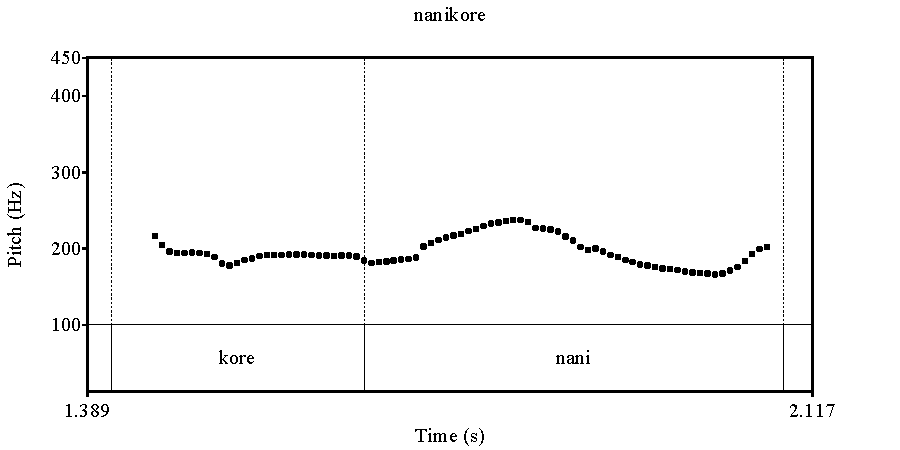
\includegraphics[width=0.6\textwidth]{sounds/korenani.pdf}
	\caption{Pitch contour of \ci{kore nani} \ref{korenani} with rising intonation}
	\label{korenaniF}
	\end{center}
%\end{minipage}
\end{figure}
\begin{figure}
%\begin{minipage}{0.5\textwidth}
	\begin{center}
	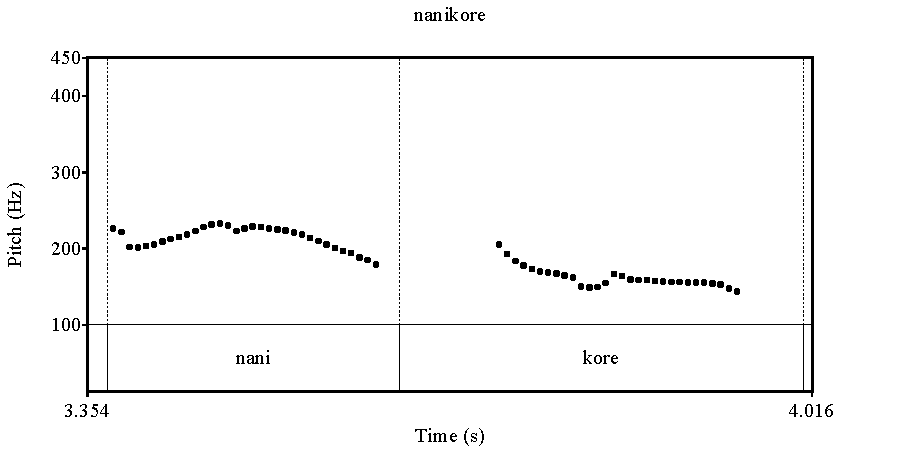
\includegraphics[width=0.6\textwidth]{sounds/nanikore.pdf}
	\caption{Pitch contour of \ci{nani kore} \ref{nanikore}}
	\label{nanikoreF}
	\end{center}
%\end{minipage}
\end{figure}
\begin{figure}
%\begin{minipage}{0.5\textwidth}
	\begin{center}
	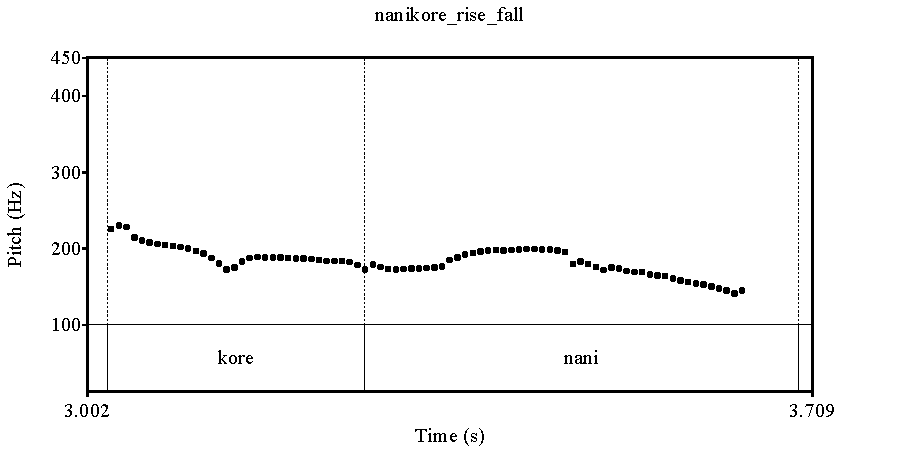
\includegraphics[width=0.6\textwidth]{sounds/korenani_fall.pdf}
	\caption{Pitch contour of \ci{kore nani} \ref{korenani} with falling intonation}
	\label{korenani_fallF}
	\end{center}
%\end{minipage}
\end{figure}
\begin{figure}
%\begin{minipage}{0.5\textwidth}
	\begin{center}
	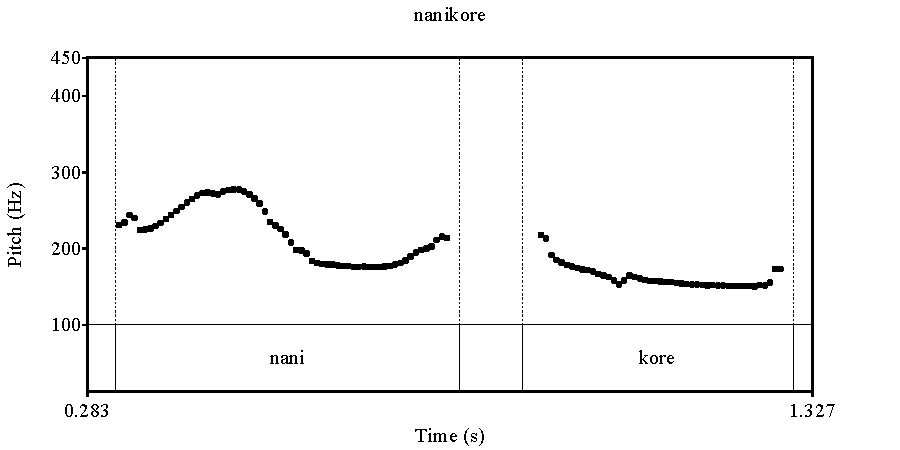
\includegraphics[width=0.6\textwidth]{sounds/nanikore_rise.pdf}
	\caption{Pitch contour of \ci{nani kore} \ref{nanikore} with rising intonation of \ci{nani}}
	\label{nanikore_riseF}
	\end{center}
%\end{minipage}
\end{figure}

%%----------------------------------------------------
\subsubsection{Post-predicate elements with double-contour type}\label{WO:PostP:Motiv:Double}

Finally, in this section,
I briefly mention intriguing studies on post-predicate constructions,
which I assume belong to double-contour type.
The first study is \citeA{kakuden12}.
They investigated whether the hearer responses (including back-channel responses) to the speaker near and after the predicate and showed that
the speaker adds post-predicate elements
when the hearer does not respond to the predicate.
Their further analysis suggests that the speaker produces post-predicate elements to acquire hearer's response and to achieve mutual belief.
Let us see example \Next,
which comes from the dialogue part of CSJ they employed.
The duration of silence is shown in second inside parentheses
since it is important for the discussion.
In \Next[-L2], where the speaker postposes the element \ci{kono kenkyuu} `this study',
there are pauses between the verb phrase and the postposed demonstrative \ci{kono} `this' and between the demonstrative and the postposed NP \ci{kenkyuu} `study',
which is enough time for L to realize that
R does not respond to L.
Note that R, the listener of the post-posed construction,
does not respond until 604.33 seconds,
0.32 seconds after L finished the post-predicate part.
Also note that
these pauses differentiate post-predicate constructions of double-contour type from those of single-contour type.
%
\ex.
 \ag.[L1:] ima nan-nin-gurai-de (0.588) a (0.29) ohi \\
           now what-\ab{cl}.person-\ab{hdg}-with {} \ab{fl} {} \ab{frg} \\
           `Right now, how many people... oh,'
 \bg.[L2:] kihontekini-wa hitori-de (0.161) \EMi{yat}-te rassyaru-desu-mon-ne
           (0.12) \EM{kono} (0.585) \EM{kenkyuu} \\
           basically-\ci{wa} alone-with {} do-and \ab{prog}.\ab{hon}-\ab{cop}-\ab{nmlz}-\ab{fp} {} this {} study \\
           `basically, (you) do (it) by yourself, this study?'
 \b.[] \src{D04M0010: 597.20-604.01}
 \bg.[R3:] ettoo (0.434) a (0.137) boku-no syozoku-si-teru kenkyuu-situ-de(0.44)-wa hanasi-kotoba-no ninsiki-o yat-teru-no-wa (0.143) m soo-desu-ne \\
           \ab{fl} {} \ab{fl} {} \ab{1}\ab{sg}-\ab{gen} belong-do-\ab{prog} study-room-\ab{loc}-\ci{wa} speech-language-\ab{gen} recognization-\ci{o} do-\ab{prog}-\ab{nmlz}-\ci{wa} {} \ab{frg} so-\ab{cop}.\ab{plt}-\ab{fp} \\
           `Lets see... in the lab I belong to, the one who studies speech recognition is, yes...,'
 \bg.[R4:] boku hitori-desu-ne \\
      \ab{1}\ab{sg} alone-\ab{cop}.\ab{plt}-\ab{fp} \\
      `it's just me.'
           \src{D04M0010: 604.33-612.09}
  \b.[] \hfill{\cite[287]{kakuden12}}
%D04M0010|00597201L|597.201362|604.007857|L|今何人ぐらいで(0.588)(F あ)(0.29)(D おひ(? てぃ))基本的には一人で(0.161)やってらっしゃる(0.207)ですもんね(0.12)この(0.585)研究||倒置−つなぎ切り
%D04M0010|00604328R|604.327743|612.085642|R|(F えっとー)(0.434)(F あ)(D (? む))(0.137)僕の所属してる研究室で(0.44)は話し言葉の認識をやってるのは(0.143)(D む)そうですね僕一人ですね|[文末候補]|


\citeA{tanaka05} investigates postposed and preposed constructions
in terms of interactional structures:
preferred vs.~dispreferred structures.
See the discussion \S \ref{Back:CharJ:WO:PostP} for detail.
%Preferred structures include assessment followed by agreement and request followed by acceptance,
%while dispreferred structures include assessment followed by disagreement and request followed by refusal.
%According to \citeA[332ff.]{levinson83},
%preferred second parts including agreement with an assessment and acceptance of a request are typically produced in a 
%simple and direct form without delay;
%on the other hand,
%dispreferred second parts including disagreement with an assessment and
%refusal of a request are typically produced in a 
%complex and indirect form with delay.
%
%%
%\ex.
% \ag.[C:] ima-no katati-to mattaku onnazi.= \\
%          now-\ab{gen} shape-with exactly same \\
%          `(It's) exactly the same shape as the ones in vogue now.'
% \bg.[K:] =onnazi-yo$\downarrow$ =[\EM{eri-mo}. \\
%          same-\ab{fp} collar-also \\
%          `(It's) the same, the collar too.'
% \bg.[E:] {\hspace{2.45cm}} [a! honto::. \\
%          {} oh really \\
%          {\hspace{2.45cm}}`Oh re::ally.'
%          \hfill{\cite[406]{tanaka05}}
%
%\ex. (A response to an inquiry about an advertisement)
% \ag. ${\uparrow}$e:to{\textasciitilde}${\downarrow}$ g{\textasciitilde} (0.3) ano:: .hhhh \\
%      uh:m {} {} uh::m \\
%      `Uh:m- g- uh::m .hhhh'
% \bg. sono $<$\ul{nakami}$>$-made \\
%      its content-as.for \\
%      `when it comes down to its contents,'
% \bg. tyotto-ne \\
%      a.bit-\ab{fp} \\
%      `sort of'
% \bg. kookoku-no$\tilde{}$ gn $>$-ga-tte-no-wa \\
%      advert-\ab{gen} \ab{frg} -\ab{nom}-\ab{quot}-\ab{nmlz}-\ab{top} \\
%      `when it comes to the (gn) of the advert,'
% \bg. tyotto \\
%      a.bit \\
%      `sort.of'r
% \bg. kotira-de-wa \\
%      here-\ab{loc}-\ab{top} \\
%      `on our side,'
% \bg. wakara-nai-n-desu-keredomo$<$, .hhhh \\
%      know-\ab{neg}-\ab{nmlz}-\ab{cop}.\ab{plt}-though \\
%      `(we) have no knowledge of, .hhhh'
%       \hfill{\cite[412-413]{tanaka05}}

%%----------------------------------------------------
\subsection{Summary of post-predicate elements}

In this section,
I investigated post-predicate elements.
It turned out that
the activation cost of postposed elements are much lower than
that of preposed elements,
which appear before the predicate.
It suggests that topics also appear post-predicatively.
I also discussed why
topics appear post-predicatively as well as clause-initially
in terms of the shape of intonation and its constraints on Japanese grammar.

The characteristic found in this study is one of many features of post-predicate elements.
In the future study,
it is necessary to explore how these features are related with each other.


%%----------------------------------------------------
%%----------------------------------------------------
\section{Pre-predicate elements}\label{WOPrePredEles}

This section discusses pre-predicate elements,
which appear immediately before the predicate.
In \S \ref{WO:PreP:New},
I show a result which indicates that
new, namely focus, elements tend to appear right before the predicate.
In \S \ref{WO:PreP:Motivation},
I discuss motivations for focus elements to appear near the predicate.

\begin{figure}
%\begin{minipage}{0.5\textwidth}
	\begin{center}
	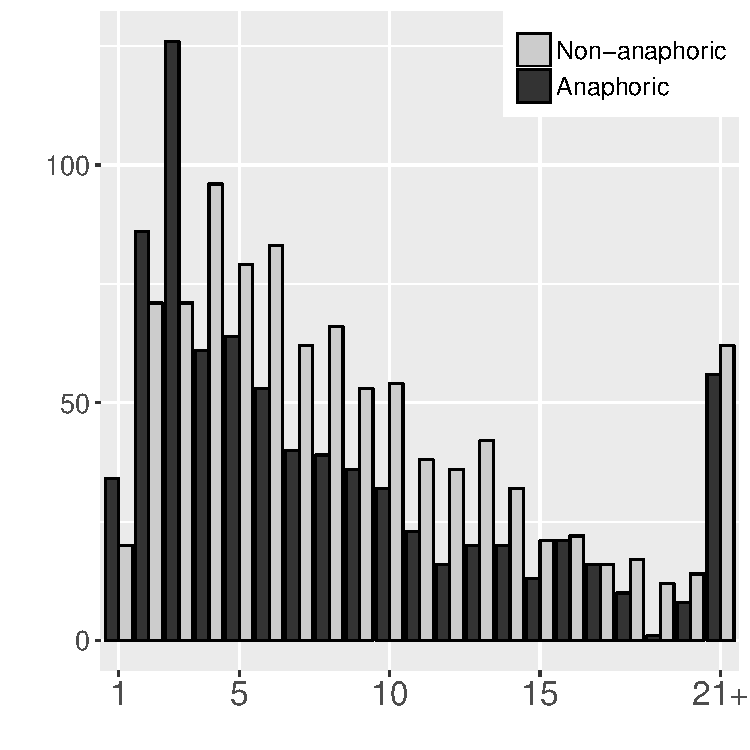
\includegraphics[width=0.7\textwidth]{figure/DEPositionIS.pdf}
	\caption{Word order vs.\ information status}
	\label{DEPositionISF2}
	\end{center}
%\end{minipage}
\end{figure}
\begin{figure}
%\begin{minipage}{0.5\textwidth}
	\begin{center}
	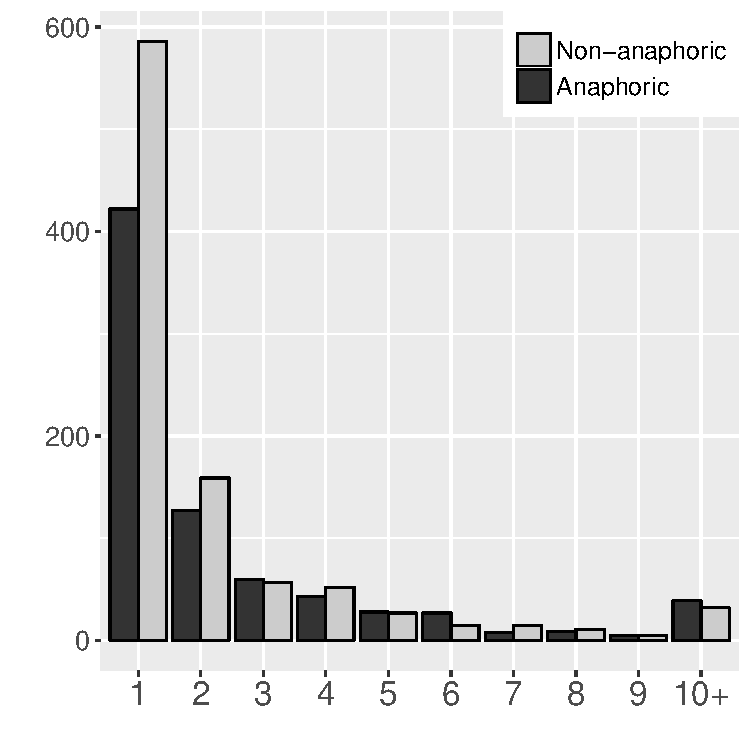
\includegraphics[width=0.7\textwidth]{figure/DiffInfoStatus.pdf}
	\caption{Distance from predicate vs.\ InfoStatus}
	\label{DiffInfoStatusF2}
	\end{center}
%\end{minipage}
\end{figure}


%%----------------------------------------------------
\subsection{New elements appear right before predicate}\label{WO:PreP:New}

%\begin{figure}
%\begin{minipage}{0.5\textwidth}
%	\begin{center}
%	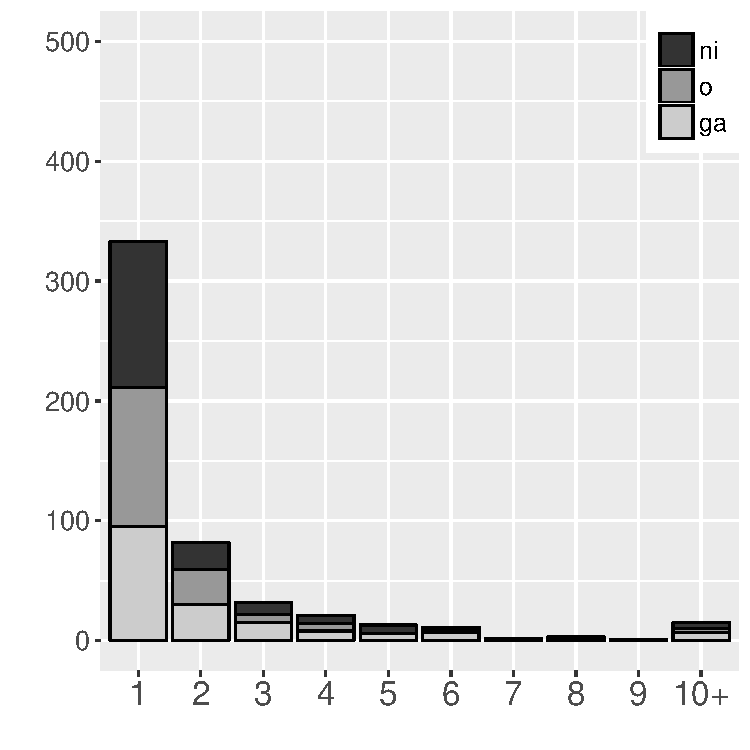
\includegraphics[width=0.95\textwidth]{figure/DiffCaseGiven.pdf}
%	\caption{}
%	\label{Diff1}
%	\end{center}
%\end{minipage}
%\begin{minipage}{0.5\textwidth}
%	\begin{center}
%	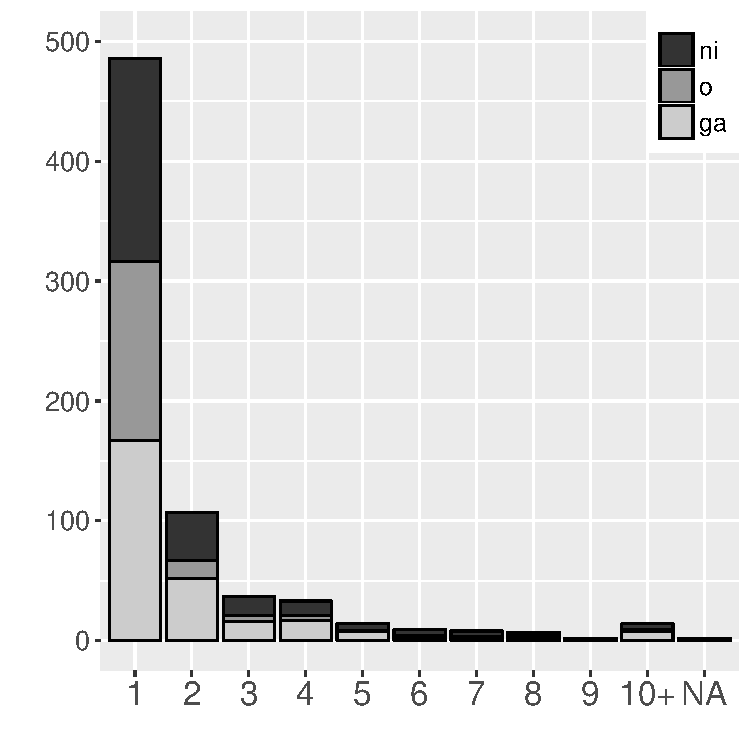
\includegraphics[width=0.95\textwidth]{figure/DiffCaseNew.pdf}
%	\caption{}
%	\label{Diff2}
%	\end{center}
%\end{minipage}
%\end{figure}
%
%\chd{
%According to the statistical analysis reported in \S \ref{WO:Intro},
%the effect of the distance between the element in question and the predicate to predict information status is only marginally significant.
%}

As shown in Figure \ref{DEPositionISF} and \ref{DiffInfoStatusF},
which are repeated here for convenience as Figure \ref{DEPositionISF2} and \ref{DiffInfoStatusF2}, respectively,
new elements or focus elements tend to appear immediately before the predicate.
Figure \ref{DEPositionISF2} shows the element position based on their information status including all expressions such as fillers, adjectives, and so on;
Figure \ref{DiffInfoStatusF2} shows the distance between the element and the predicate based on their information status.
%Figure \ref{WOISGivenF2} and \ref{WOISNewF2} are histograms of position of arguments excluding other expressions and clauses with one argument.
%They also show the distribution of A, S, and P in each position.
As indicated in Figure \ref{DEPositionISF2},
the distribution of anaphoric elements skews towards clause-initial position,
whereas that of non-anaphoric elements does not.
Taking Figure \ref{DiffInfoStatusF2} also into this account,
we can see that many of new elements appear immediately before the predicate.
%Considering clauses which contain equal to or more than two arguments,
%given elements appear at the initial position most frequently
%as shown in Figure \ref{WOISGivenF2},
%whereas new elements appear at the second position most frequently as shown \ref{WOISNewF2}.
%Especially given A elements are more frequent than new A elements in the initial position.
%This is compatible with the observation that A tend to be given in Sakapultec Maya and many other languages \cite{dubois87,duboisetal03}.
%New S or P elements appear more frequently than given S or P elements in the second position.
\chd{As discussed in \ref{WO:Intro}, the mixed effects model of information status (the distance between the predicate and the element in question) shows that
the contribution of the distance is only marginally significant.
However, a further analysis imply that the distance is also a significant factor to predict information status.
As is clear from Table \ref{ParInfoStatusCTT} and \ref{Par:InfoStatusPar:LSMEANST},
datives tend to code new elements (especially, as opposed to \ci{wa}).
Datives can appear anywhere, from pre-predicate to clause-initial positions,
which is shown in Figure \ref{WO:Prep:New:DiffASPF}.
%In fact, the model excluding datives indicates that
%both the distance and particles are significant factors to predict information status (likelihood ratio test, $p<0.05$ without the distance, $p<0.001$ without particles).
Therefore, I tantatively conclude that the distance between the predicate and the element in question (excluding \ci{ni}-coded elements) is an important factor for information status and
new elements appear before the predicate.
This supports a classic observation in other languages that focus appears closely with the predicate (\citeA{bresnan94,morimoto99} on Bantu languages, \citeA{jacennikdryer92} on Polish, \citeA{erguvanli84} on Turkish, see \citeA{morimoto00} for the summary of studies on both VO and OV languages).
Further studies are necessary to obtain conclusive evidence.}

\begin{figure}
	\begin{center}
	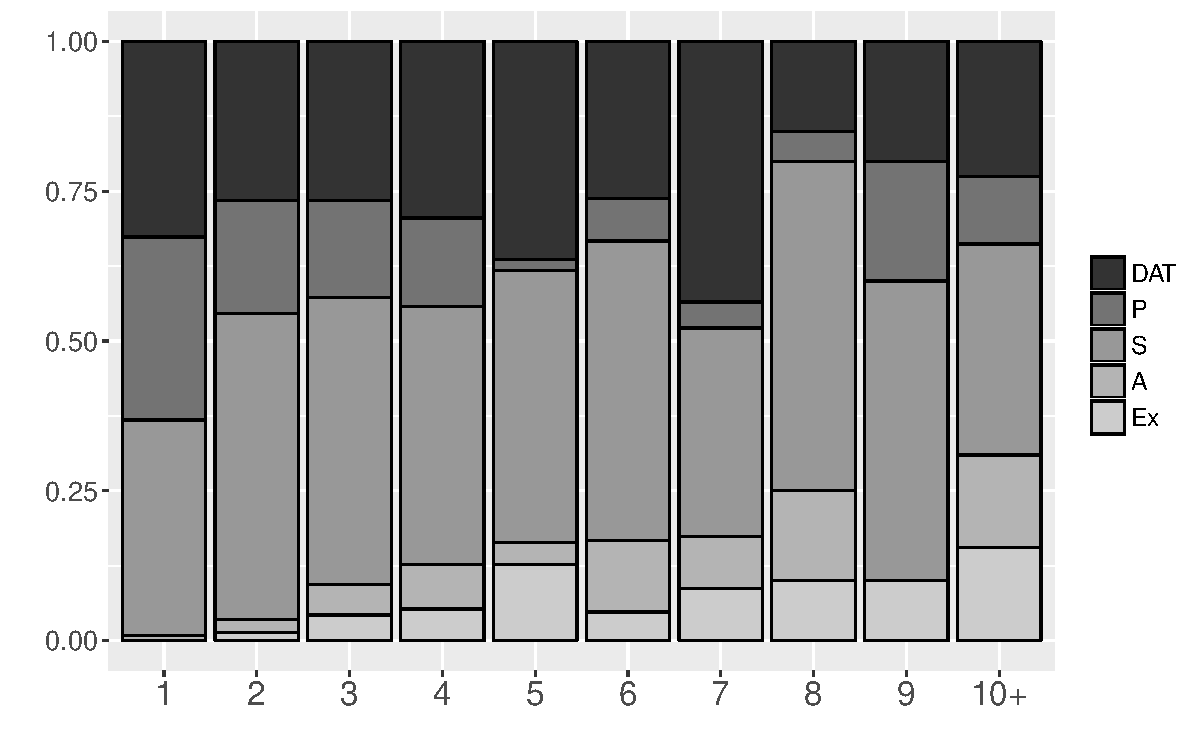
\includegraphics[width=0.8\textwidth]{figure/DiffASP.pdf}
	\caption{Distance from predicate vs.~grammatical functions}
	\label{WO:Prep:New:DiffASPF}
	\end{center}
\end{figure}


The following are example of non-anaphoric elements appearing close to the predicate.
\Next and \NNext are examples of non-anaphoric P occurring immediately before the predicate.
In \Next,
\ci{kyoomi} `interest' appear immediately before the predicate \ci{moti} `have',
and, in \NNext,
\ci{aidenthithii} `identity' in line a, \ci{inoti} `life' in line b, and \ci{ti} `blood' in line c appear right before the preciates \ci{kake} `risk' and \ci{nagasi} `bleed', respectively.
Non-anaphoric Ps are typically abstract concepts like \ci{kyoomi} `interest' in \Next, \ci{aidenthithii} `identity' in \NNext[a], and \ci{inoti} `life' in \NNext[b], or
indefinite like \ci{ti} `blood' in \NNext[c].
%
\exg. de ee sono ri-too-no hoo-ni sono \EM{kyoomi-o} \ul{moti} hazime-masi-te \\
		then \ab{fl} \ab{fl} remote-island-\ab{gen} direction-\ab{dat} \ab{fl} interest-\ci{o} have start-\ab{plt}-and \\
	`(We) are started to be interested in remote islands (in Hawaii).'
	\src{S00F0014: 149.92-153.33}
%S00F0014|00149920L|149.919959|153.334445|L|で(0.325)(F えー)(F その)離島の方に(F その)興味を持ち始めまして|/テ節/|

\ex.\label{S00M0199_inoti}
 \ag. tasuu-no serubia-zin-ga minzoku-no ee \EM{aidenthithii-o} \ul{kake}-te \\
 	many-\ab{gen} Serbia-people-\ci{ga} ethnic-\ab{gen} \ab{fl} identity-\ci{o} risk-and \\
	`Serbian people bet their identity, and'
 \bg. \EM{inoti-o} \ul{kake}-te \\
 		life-\ci{o} risk-and \\
		`risked their lives, and'
 \bg. \EM{ti-o} \ul{nagasi}-ta-to iu \\
 		blood-\ci{o} bleed-\ab{past}-\ab{q} say \\
		`bled (in battles),'
 \bg. rekisi-ga ee sono-go tenkai s-are-masu \\
 	history-\ci{ga} \ab{fl} that-later progress do-\ab{pass}-\ab{plt} \\
	`the history went on this way.'
	\src{S00M0199: 343.53-351.77}
%S00M0199|00337016L|337.015835|351.772351|L|その時(0.488)(F えー)(F ま)その聖地(0.157)を(0.142)守るという意味で(F あのー)このコソボ平原において(0.422)(F えー)多数のセルビア人が民族の(0.204)(F えー)アイデンティティーを賭けて命を賭けて血を流したという(0.379)歴史が(0.17)(F えー)その後(0.167)展開されます|[文末]|

Non-anaphoric S elements also appear immediately before the predicate.
They tend to be abstract or indefinite like non-anaphoric Ps.
In \Next,
\ci{kanzi} `impression' is the only argument of the predicate \ci{tigau} `differ' and hence is S,
which is an abstract concept.
This appears immediately before the predicate.
%
\ex.\label{S00F0014_kanzi}
 \ag. sono kontorasuto-toiuno-wa nanka totemo koo ekizotikku-to-iu-ka \\
 	that contrast-\ci{toiuno}-\ci{wa} somehow very such exotic-\ab{quot}-say-\ab{q} \\
	`The contrast (the color of black and blue) is very exotic, I would say,'
 \bg. husigina \EM{kanzi}-ga \ul{si}-masi-te \\
 		mysterious impression-\ci{ga} do-\ab{plt}-and \\
		`the impression was mysterious.'
		\src{S00F0014: 1042.88-1047.03}
%S00F0014|01042882L|1042.88247|1047.031717|L|そのコントラストというのは何かとてもこうエキゾチックと言うか不思議な感じがしまして|/テ節/|
%
%\ex.
% \ag. iya risu-nisite-wa tyotto sippo-no \EM{kanzi}-ga tigau-na-to \\
% 		no squirrel-for-\ci{wa} a.bit tail-\ab{gen} impression-\ab{nom} different-\ab{fp}-\ab{quot} \\
%		`No, the impression of (the animal's) tail is different from that of squirrels,'
% \bg. omot-te-ta-n-desu-ne \\
% 	think-\ab{prog}-\ab{nmlz}-\ab{cop}.\ab{plt}-\ab{fp} \\
%	`(I) was thinking like that.'
%	\src{S00F0014: 635.38-639.92}
%S00F0014|00635381L|635.381427|639.920666|L|いやリスにしてはちょっと尻尾の感じが違うなと(0.352)思ってたんですね|[文末]|

In \Next,
\ci{hito} `person' is indefinite and appears before the predicate.
\exg. naka-ni-wa byooin-okuri-ni naru \EM{hito}-mo \ul{i}-masi-ta-kedomo \\
		inside-\ab{dat}-\ci{wa} hospital-send-to become person-also exist-\ab{plt}-\ab{past}-though \\
		`Some people were sent to the hospital (lit. People who were sent to the hospital also exist).'
		\src{S05M1236: 578.30-581.49}
%S05M1236|00578305L|578.304793|581.489255|L|中には病院送りになる(0.445)<笑>人もいましたけども|/並列節ケドモ/|


%%----------------------------------------------------
\subsection{Motivations for focus to appear close to predicate}\label{WO:PreP:Motivation}

%Why do non-anaphoric elements most frequently appear close to the predicate?
I argue that the information-structure continuity principle \ref{IScontinuityP} is also at work here, which is repeated below as \Next for the purpose of convenience.
%
\ex. \label{IScontinuityP2}\tl{Information-structure continuity principle}:
 A unit of information structure is continuous in a clause;
 i.e., elements which belong to the same unit are adjacent with each other.

I assume that
most frequently the predicate is in the domain of focus \cite{lambrecht94},
optionally with one focus element.
Since the predicate and the new element are in the same domain of focus,
they appear together most frequently.

In fact, few studies pay attention to the information status (and namely information structure) of predicates.%
	\footnote{
	\citeA{hopperthompson80} is an important exception.
	}
Unfortunately this study is not an exception.
Typically definite markers such as \ci{the} in English and \ci{der} in German attach to nouns, not to verbs.
Also topic markers such as \ci{wa} in Japanese typically attach to nouns.
Therefore, nouns have attracted more attention than verbs.
Typically verbs are followed by tense or aspect markers, subordinate-clause markers, realis vs.\ irrealis markers, and so on.
I believe that these verbal markers are also related to information structure,
but this is beyond the scope of this study.

However,
it is obvious that argument-focus structure,
where the predicate is not in the domain of focus,
is the least frequent type among all three types (predicate-focus, sentence-focus, and argument-focus structures).
Especially the corpus employed in this study is monologues,
there are expected to be even fewer examples of argument-focus structures
because argument-focus structure typically appears as the answer to a question of \ci{who/what} as shown in \Next,
where the capital letters indicate prominence.
%
\ex.
 \a.[Q:] Who went to school?
 \b.[A:] [The CHILDREN]$_{F}$ [went to school]$_{T}$.
 \hfill{\cite[][p.~121]{lambrecht94}}

Since there are no (explicit) questions in monologues,
there are few argument-focus structure.

Another context in which sentences of argument-focus structure appear is ``A not B'' context.
In monologue, ``A not B'' context typically appears in self-repair,
which is also rare in our relatively smooth monologues.
Therefore, it is not unreasonable to assume that the predicate is in the domain of focus most of the time,
and I argue that the information-structure continuity principle \ref{IScontinuityP2} explains why new elements (i.e., focus elements) tend to appear immediately before the predicate.

One piece of evidence that supports the information-structure continuity principle is the fact that
it is difficult for presupposed elements to appear immediately before the predicate,
intervening the focus domain.
Compare \Next[A] and \Next[A$^{\prime}$],
which are assumed to be the answers to the question \Next[Q].%
	\footnote{
	Note that they are not a perfect minimal pair because of the accusative marker of \ci{o}.
	The presence or absence of \ci{o} is determined by word order and
	information structure is a kind of side effect in this case.
	See the discussion in \S \ref{CasePar} for more detail.
	}
In \Next[A],
the presupposed elements \ci{taroo-ni} `to Taro' and \ci{hanako-ni} `to Hanako' are intervening the domain of focus `gave a travel ticket' and `gave a cake'.
Therefore this sentence is not acceptable.
Contrarily, in \Next[A$^{\prime}$],
the presupposed elements do not intervene the domain of focus and hence this is acceptable.
%
\ex.
 \a.[Q:] What did you do for Taro and Hanako for their birthdays?
 \bg.[A:] ?[ryokoo-ken-o]$_{F}$ [taroo-ni]$_{T}$ [age-te]$_{F}$ [keeki-o]$_{F}$ [hanako-ni]$_{T}$ [tukut-te age-ta]$_{F}$-yo \\
 			travel-ticket-\ci{o} Taro-\ab{dat} give-and cake-\ci{o} Hanako-\ab{dat} make-and give-\ab{past}-\ab{fp} \\
			`(I) gave travel tickets to Taro and gave cake to Hanako.'
 \bg.[A$^{\prime}$:] [taroo-ni]$_{T}$ [ryokoo-ken age-te]$_{F}$ [hanako-ni]$_{T}$ [keeki tukut-te age-ta]$_{F}$-yo \\
 			Taro-\ab{dat} travel-ticket give-and Hanako-\ab{dat} cake make-and give-\ab{past}-\ab{fp} \\
			`(I) gave travel Taro travel tickets and gave Hanako cake.'

A more natural context for \Last[A] is where Q asks
what A did for the travel ticket and the cake.
\citeA{kuno78} proposes that
the pre-predicate position is for new elements,
but he limits this principle to cases
where the predicate is given.
%
\ex.
 In cases where the predicate is given,
 the position immediately before the predicate is the position for new.
 \hfill{\cite[][p.~60, translated by the current author]{kuno78}}

I argue that this observation also applies to cases where the predicate is new.

Moreover,
as will be discussed in Chapter \ref{Intonation},
the domain of focus is uttered in a single intonation unit,
whereas the topic is uttered separately from the domain of focus.
Figure \ref{S00M0199_aidenthithiF} to \ref{S00F0014_kanziF} show
the pitch contours of examples \ref{S00M0199_inoti} and \ref{S00F0014_kanzi} we discussed in the last section.
As we can see,
there is no pause between the predicate and the previous element and
the pitch range is larger in the elements than in the predicates.
In Figure \ref{S00M0199_tiF},
it is difficult to see the pitch range because \ci{ti} `blood' does not have accent nucleus.
From the first lowering of \ci{na} in \ci{nagasi-ta} `bled' being cancelled,%
	\footnote{
	The pitch accent of \ci{nagasi-ta} is LHLL.
	}
one can see that
\ci{ti-o} `blood-\ci{o}' and \ci{nagasi-ta} `bleed' form a single intonation unit.


\begin{figure}
%\begin{minipage}{0.5\textwidth}
	\begin{center}
	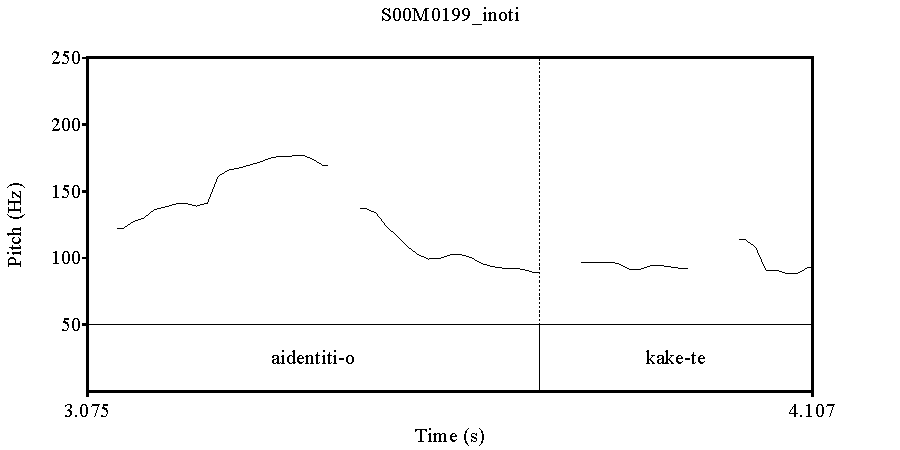
\includegraphics[width=0.6\textwidth]{sounds/S00M0199_aidenthithi.pdf}
	\caption{Pitch contour of a in \ref{S00M0199_inoti}}
	\label{S00M0199_aidenthithiF}
	\end{center}
%\end{minipage}
\end{figure}
\begin{figure}
%\begin{minipage}{0.5\textwidth}
	\begin{center}
	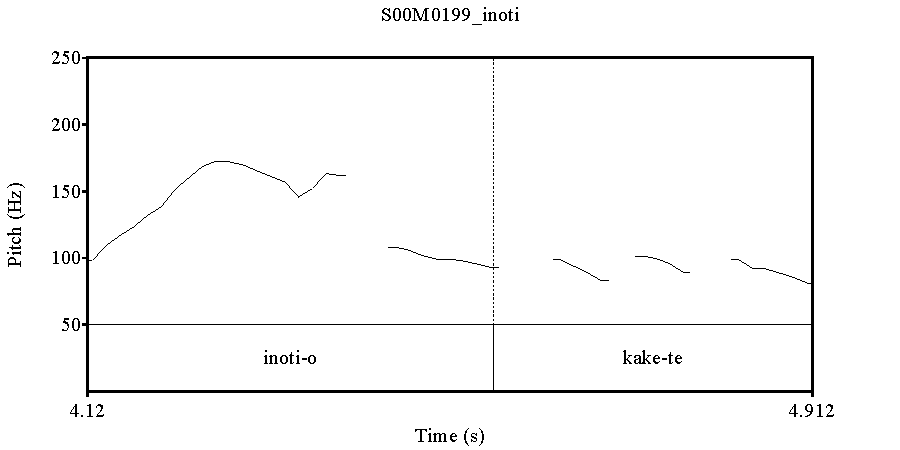
\includegraphics[width=0.6\textwidth]{sounds/S00M0199_inoti.pdf}
	\caption{Pitch contour of b in \ref{S00M0199_inoti}}
	\label{S00M0199_inotiF}
	\end{center}
%\end{minipage}
\end{figure}
\begin{figure}
%\begin{minipage}{0.5\textwidth}
	\begin{center}
	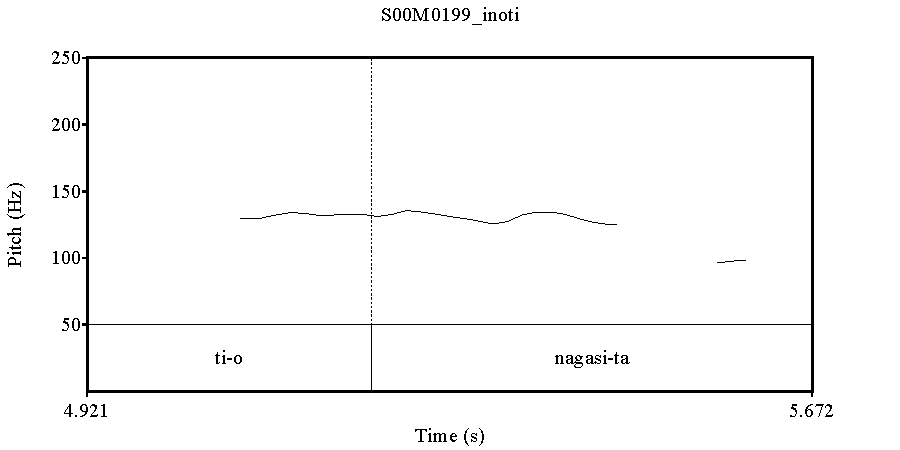
\includegraphics[width=0.6\textwidth]{sounds/S00M0199_ti.pdf}
	\caption{Pitch contour of c in \ref{S00M0199_inoti}}
	\label{S00M0199_tiF}
	\end{center}
%\end{minipage}
\end{figure}
\begin{figure}
%\begin{minipage}{0.5\textwidth}
	\begin{center}
	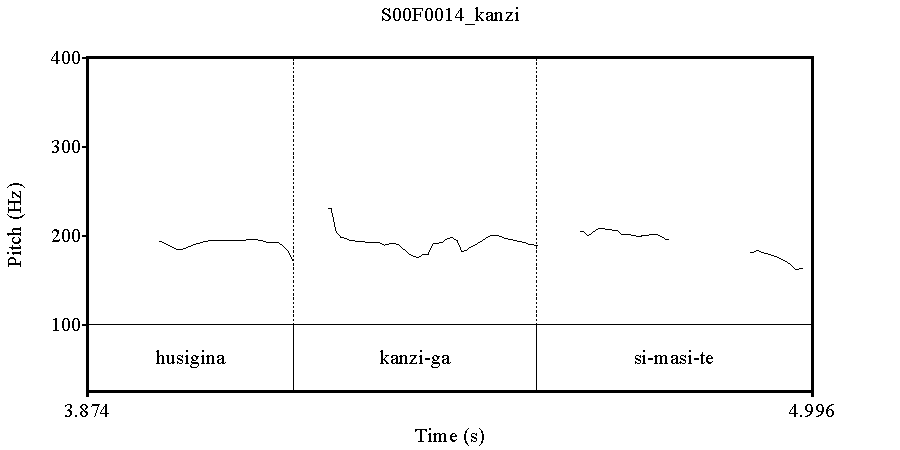
\includegraphics[width=0.6\textwidth]{sounds/S00F0014_kanzi.pdf}
	\caption{Pitch contour of b in \ref{S00F0014_kanzi}}
	\label{S00F0014_kanziF}
	\end{center}
%\end{minipage}
\end{figure}

%%----------------------------------------------------
\subsection{Summary of pre-predicate elements}

The results of this section showed that
new, namely focus, elements tend to appear right before the predicate.
A similar claim has been made by \citeA{kuno78} and \citeA{endo14}
through constructed examples.
This study supported their claim by examining natural occurring utterances.
I also discussed motivations for focus to appear right before the predicate.

%%----------------------------------------------------
%%----------------------------------------------------
\section{Discussion}\label{WODiscussion}

This section first discusses possible confounding effects on word order in Japanese,
especially in association with basic word order (\S \ref{WO:Dis:Confounding}).
Second,
I discuss Giv{\'{o}}n's topicality hierarchy (\S \ref{WO:Dis:Givon}).
I provide some counter-examples of this hierarchy and
propose to modify it.
Finally, 
I discuss the implications of this study's findings toward word order typology (\S \ref{WO:Dis:WOTypology}).



%%----------------------------------------------------
\subsection{Possible confounding effects}\label{WO:Dis:Confounding}

\begin{figure}
%\begin{minipage}{0.5\textwidth}
	\begin{center}
	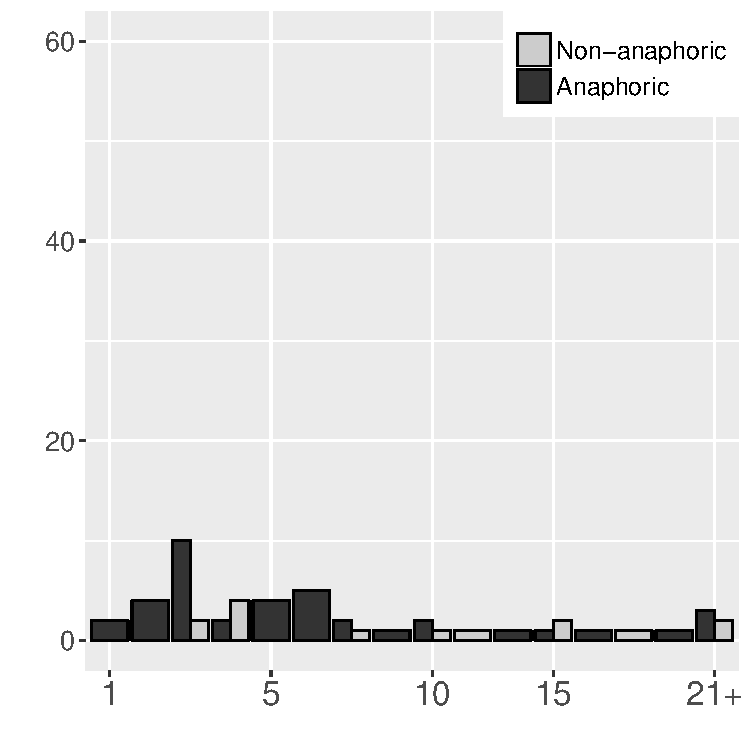
\includegraphics[width=0.6\textwidth]{figure/DEPositionASPA.pdf}
	\caption{Word order of A}
	\label{DEPositionASPAF}
	\end{center}
%\end{minipage}
\end{figure}
\begin{figure}
%\begin{minipage}{0.5\textwidth}
	\begin{center}
	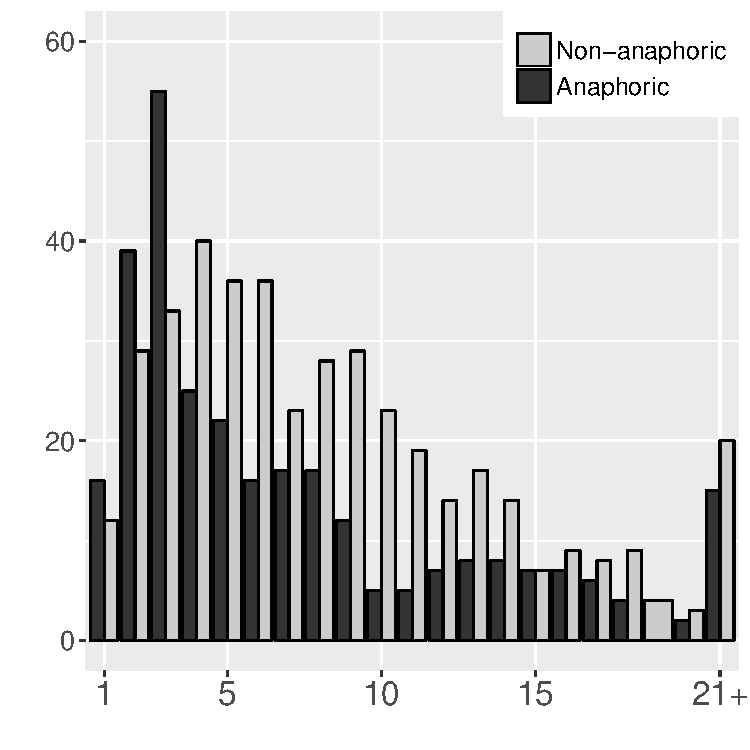
\includegraphics[width=0.6\textwidth]{figure/DEPositionASPS.pdf}
	\caption{Word order of S}
	\label{DEPositionASPSF}
	\end{center}
%\end{minipage}
\end{figure}
\begin{figure}
%\begin{minipage}{0.5\textwidth}
	\begin{center}
	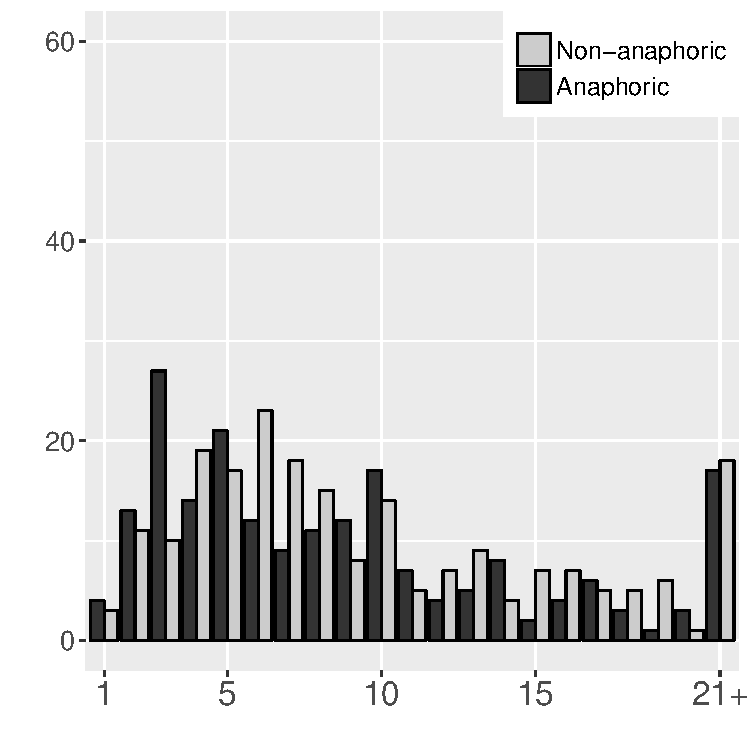
\includegraphics[width=0.6\textwidth]{figure/DEPositionASPP.pdf}
	\caption{Word order of P}
	\label{DEPositionASPPF}
	\end{center}
%\end{minipage}
\end{figure}
\begin{figure}
%\begin{minipage}{0.5\textwidth}
	\begin{center}
	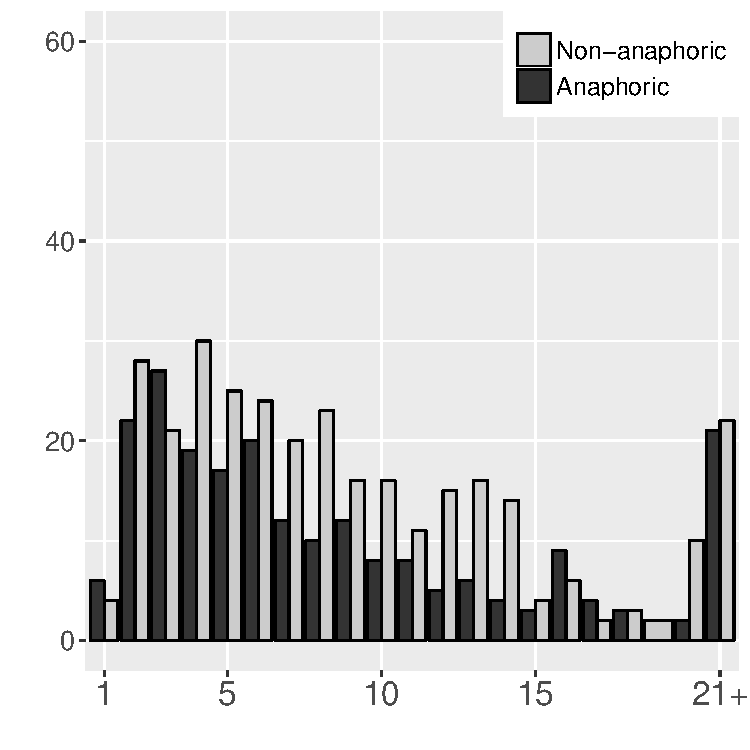
\includegraphics[width=0.6\textwidth]{figure/DEPositionASPDAT.pdf}
	\caption{Word order of dative}
	\label{DEPositionASPDATF}
	\end{center}
%\end{minipage}
\end{figure}


It is necessary to take other features into account
to see the exact effect of topichood and focushood on word order.
Especially, the effect of ``basic word order'' should not be ignored.
%I did not employ any statistical analysis because
%there are still not enough data in my corpus.
Here I provide some evidence to support my argument that
information structure contributes to word order in spoken Japanese.
Figure \ref{DEPositionASPAF} to \ref{DEPositionASPDATF} show
word order and information status of each type of grammatical function (A, S, P, and dative).
These figures indicate that
anaphoric elements of all grammatical function types are still more likely to appear earlier in a clause than new elements.
A and S are more likely to appear earlier in a clause than P because of the basic word order.
However, my argument still holds for the same grammatical function types.
In case with new elements,
one can see the effect of basic word order;
the peak of S is 4,
which means the 4th position is the most popular for new S (Figure \ref{DEPositionASPSF}),
whereas the peak of P is 6, which means the 6th position is the most popular for new P (Figure \ref{DEPositionASPPF}).
The distribution of A is not clear because there are few examples.
But the trend still seems to hold for A.

%%----------------------------------------------------
\subsection{Giv\'on's topicality hierarchy and word order}\label{WO:Dis:Givon}

\citeA{givon83} proposes a hierarchy of topicality \Next (terminology modified by the author).
``RD'' refers to referential distance,
which is one of the approximations to measure topicality.
Low RD means high topicality,
while high RD means low topicality.
%
\ex.\label{TopicHierarchy}
 \a.[$\uparrow$] High RD
 \b. Referential indefinite NPs
 \b. Cleft/focus constructions
 \b. Y-moved NPs (`contrastive topicalization')
 \b. Preposed definite NPs
 \b. Neutral-ordered definite NPs
 \b. Postposed definite NPs
 \b. Stressed/independent pronouns
 \b. Unstressed/bound pronouns or grammatical agreement
 \b. Zero anaphora
 \b.[$\downarrow$] Low RD
 \hfill{\cite[][p.~7]{givon83}}

Here I point out two counter-examples against this hierarchy.
First,
as has already been shown in Table \ref{RDPostT} and \ref{RDPreT},
which are repeated as Table \ref{RDPostT2} and \ref{RDPreT2} for convenience,
the average RD of elements in the clause-initial position (20.9) is lower than that in the second (23.0) or third positions (41.1).
To see this more in detail,
I divided the result of Table \ref{RDPreT2} based on grammatical function.
This is shown in Table \ref{RDASP}.
Regardless of whether the element is A, S, or P,
the overall tendency is that
the elements closer to the predicate have higher average RD.%
 \footnote{
 For now I do not have an explanation for S in the second position.
 It is necessary to test whether the difference between Ss in the first and the second positions are statistically significant or not.
 }
%%% 2Sに関しては説明が必要
The topicality hierarchy \ref{TopicHierarchy} predicts that
clause-initial elements (d in \ref{TopicHierarchy}) is lower RD than elements in the neutral-ordered position (e in \ref{TopicHierarchy}).%
	\footnote{
	I assume that all elements that have antecedents (and namely RDs) are definite.
	}
Especially P is against the topicality hierarchy \ref{TopicHierarchy},
according to which P in the second or third positions should have lower RD than P in the first position because the neutral position of P is the second or third positions in Japanese.
But this is not the case.
At least in Japanese,
the data show that
elements closer to the predicate have higher RDs
because the pre-predicate position is for focus and hence new elements.

\begin{table}[bht]
%\begin{minipage}{0.5\textwidth}
\centering
\caption{RD of post-predicate elements}
\begin{tabular}{lrr}
\toprule
  & Single-contour & Double-contour \\
\midrule
RD & 6.9 & 39.7 \\
\bottomrule
\end{tabular}
\label{RDPostT2}
%\end{minipage}
\end{table}
\begin{table}
%\begin{minipage}{0.5\textwidth}
\centering
\caption{RD of pre-predicate elements (based on argument order)}
\begin{tabular}{lrrrr}
\toprule
  &  1  & 2 & 3 \\
\midrule
RD & 20.9 & 23.0 & 41.1 \\
\bottomrule
\end{tabular}
\label{RDPreT2}
%\end{minipage}
\end{table}

\begin{table}
%\begin{minipage}{0.5\textwidth}
\centering
\caption{RD of pre-predicate elements (based on grammatical function)}
\label{RDASP}
\begin{tabular}{lrrr}
\toprule
		& 1	& 2	& 3 \\
\midrule
%	Ex	& 15.2	& 15.0 & --	\\
	A	& 10.3	& 47.3	& -- \\
	S	& 22.5	& 21.7	& 73.5 \\
	P	& 22.4	& 36.6	& 49.1 \\
\bottomrule
\end{tabular}
%\end{minipage}
\end{table}

Second,
the average RD of zero pronouns is as high as that of postposed NPs
according to Table \ref{RDPostExpTypeT} and \ref{RDPreExpTypeT}.
This is against the topicality hierarchy \ref{TopicHierarchy}
because it states that
preposed definite NPs (d in \ref{TopicHierarchy}) and neutral-ordered definite NPs (e in \ref{TopicHierarchy}) have
higher RDs than
postposed definite NPs.
As discussed above,
elements are postposed for some interactional purpose and/or intonational reason.


\begin{table}
%\begin{minipage}{0.5\textwidth}
\centering
\caption{RD of postposed elements of single-contour type (based on expression type)}
\begin{tabular}{lrr}
\toprule
  & Pronoun & NP \\
\midrule
RD & 15.1 & 5.0 \\
\bottomrule
\end{tabular}
\label{RDPostExpTypeT}
%\end{minipage}
\end{table}
\begin{table}
%\begin{minipage}{0.5\textwidth}
\centering
\caption{RD of pre-predicate elements (based on expression type)}
\begin{tabular}{lrrr}
\toprule
     & Zero & Pronoun & NP \\
\midrule
 RD  & 5.0  & 5.8     & 27.8 \\
\bottomrule
\end{tabular}
\label{RDPreExpTypeT}
%\end{minipage}
\end{table}

The final point is an additional suggestion of \ref{TopicHierarchy} rather than a counter-example.
The RD of postposed elements of double-contour type is much higher than Giv\'on predicts.
As will be argued in Chapter \ref{Intonation},
a unit of information structure corresponds to a unit of intonation.
Since postposed elements of single-contour type by definition belong to the same intonation unit as the main predicate,
the predicate and the postposed element form a single unit (construction) and postposed elements are relatively homogeneous and are relatively easy to characterize.
However,
postposed elements of double-contour type are heterogeneous as discussed above and are difficult to characterize
because the element itself corresponds to a single unit.
The motivations for such elements to be uttered are heterogeneous.
The functions of such postposed elements are determined by the sequence of conversation.


%%----------------------------------------------------
\subsection{Information structure and word order typology}\label{WO:Dis:WOTypology}

Since most frequent focus elements are patients according to the correlating features \ref{ISFeatures},
which is repeated as \Next,
the information-structure continuity principle \ref{IScontinuityP} predicts that cross-linguistically
P (the patient-like argument in a transitive clause) and V (the predicate) tend to appear together most frequently and,
if the word order is fixed in the language in question,
P and V tend to appear together.
%
\ex.
\begin{tabular}{lll}
	 & topic & focus \\
	a. & presupposed & asserted \\
	b. & evoked & brand-new \\
	c. & definite & indefinite \\
	d. & specific & non-specific \\
	e. & animate & inanimate \\
	f. & agent & patient \\
	g. & inferable & non-inferable \\
%	h. & entity & proposition \\
\end{tabular}
%

In fact this has already been claimed and tested in \citeA[Chapter 4]{tomlin86}.
Tomlin proposes this claim as Verb-Object Bonding.
%
\ex. \tl{Verb-Object Bonding (VOB):}
	the object of a transitive verb is more tightly bounded to the verb
	than is its subject.
	\hfill{\cite[][p.~74]{tomlin86}}
%``[i]n general the object of a transitive clause is syntactically and semantically more tightly `bound' to the verb than is the subject of a transitive clause'' (p.~73).

He also states that
``[e]xactly why there should be such a bond between a transitive verb and its object is not entirely clear'' (ibid.).
I propose the information-structure continuity principle
for the motivation of such bond.
He enumerates many cross-linguistic pieces of evidence that support VOB.
I introduce a few of them to keep the discussion simple.

First,
in many languages,
there exists some clause-level phonological behavior
(reductions or sandhis) which occur between object and verb,
but not between subject and verb (op.~cit., p.~97).
In French, for example,
liaison does not occur between the subject and the transitive verb,
but it does between the object and the verb \cite[see also][]{selkirk72}.
There is no liaison between the subject \ci{les gens} and the verb \ci{ach\`{e}tent} as in \Next,
whereas there can be liaison between the verb \ci{donnerons} and the object \ci{une pomme} as in \NNext.
%
\ex.
 \a. \glll
	les gens ach\`{e}tent beaucoup de \c{c}a \\
	\tp{le} \tp{Z\~a} \tp{aSEt} \tp{boku} \tp{d@} \tp{sa} \\
	the people buy much of that \\
	`Those people buy a lot of that.' \hfill{(no liaison)}
 \b. *\tp{le} \tp{Z\~a} \tp{zaSEt} \tp{boku} \tp{d@} \tp{sa} 
 		 \hfill{(*liaison)}

\ex.
 \a. \glll
	nous donnerons une pomme \`a notre m\`ere \\
  	\tp{nu} \tp{dOn@r\~o} \tp{zyn} \tp{pOm} \tp{a} \tp{notr} \tp{mEr} \\
	we give.\ab{3}\ab{pl} a apple to our mother \\
	`We will give an apple to our mother.'
	\hfill{(liaison)}
\begin{flushright}
\cite[][pp.~98-99, transcription modified based on standard French]{tomlin86}
\end{flushright}

Another case is Yoruba (Niger-Congo) vowel deletion \cite[from][]{bamgbose64}.
In verb-noun sequences of this language,
when the object begins with a vowel,
the last vowel of the verb is sometimes deleted.
This happens between verb and object, but not between subject and verb.
%
\ex.
 \ag. \tp{gb\'e} + \tp{od\'o} $\to$ \tp{gb'\'od\'o} \\
		brought + motor \\
 \bg. \tp{jE} \tp{iy\'On} $\to$ \tp{j'iy\'On} \\
 		eat pounded.yam \\
 \bg. \tp{Se} \tp{\`ow\`o} $\to$ \tp{S'\`ow\`o} \\
 		do trade \\
		\hfill{\cite[][pp.~29--30]{bamgbose64}}

These phonological phenomena in French and Yoruba suggest that
the object and predicate are bound tighter than the subject and predicate.
In a similar manner,
in Japanese,
the focus element and the predicate form a single intonation unit,
but the topic element and the predicate do not,
as we will see in Chapter \ref{Intonation}.

The second piece of evidence that supports VOB is noun incorporation.
In Mokilese (Oceanic), for example,
there is a set of verbs into which an indefinite object may be incorporated \cite[from][]{harrison76}.
\Next[a] is a transitive clause with definite object,
which is not incorporated into the verb,
whereas \Next[b] is a clause with indefinite object,
which is incorporated into the verb.
Note that the incorporate object \ci{rimeh} `bottle' in \Next[b] is between the verb and the aspect suffix \ci{la}.
%
\ex.
 \ag. ngoah audoh-\EMi{la} \EM{rimeh}-i \\
		\ab{1}\ab{sg} fill-\ab{pfv} bottle-this \\
		`I filled this bottle.'
 \bg. ngoah audohd \EM{rimeh}-\EMi{la} \\
		\ab{1}\ab{sg} fill bottle-\ab{pfv} \\
		`I filled bottles.'
		\hfill{\cite[162]{harrison76}}

Similarly,
compare \Next[a] and \Next[b].
\Next[a] is a case where the object \ci{suhkoah} `tree' is definite and is not incorporated,
while \Next[b] is a case where the object is indefinite and is incorporated into the verb.
\ex.
 \ag. ngoah poadok-\EMi{di} \EM{suhkoah}-i \\
 	\ab{1}\ab{sg} plant-\ab{pfv} tree-this \\
	`I planted this tree'
 \bg. ngoah poad \EM{suhkoah}-\EMi{di} \\
 	\ab{1}\ab{sg} plant tree-\ab{pfv} \\
	`I planted trees.'
	\hfill{(ibid.)}

As \citeA{mithun84} observes,
in some languages patient S can also be incorporated into verbs
but languages allows patient S-incorporation also allows P-incorporation (See also \citeA{baker88}).
Namely, there is a universal hierarchy as in \Next.
The last two (agent S and A) are in brackets because
they are not attested.
%
\ex. \label{NIhierarchy}P $>$ patient S ($>$ agent S $>$ A)

In Southern Tiwa (Tanoan), for example,
the patient Ss `dipper' and `snow' are incorporated as in \Next,
while the agent Ss such as `dog' cannot be incorporated as in \NNext.
	\ex. \ag. \tp{l-\EM{k'uru}-k'euwe-m} \\
			{\sc B}-\EM{dipper}-old-\ab{pres} \\
			`The dipper is old.'
		\bg. \tp{we-\EM{fan}-lur-mi} \\
			{\sc C}.\ab{neg}-\EM{snow}-fall-\ab{pres}.\ab{neg} \\
			`Snow isn't falling. (It is not snowing.)'  \hfill{(patient S)}
		\b.[] \hfill{\cite{allenetal84,baker88}}
	
	\ex. \ag. \tp{\EM{khwien}-ide} \tp{{\O}-teurawe-we} \\
			\EM{dog}-{\sc suf} {\sc A}-run-\ab{pres} \\
			`The dog is running.'
		\bg. *\tp{{\O}-\EM{khwien}-teurawe-we} \\
			{\sc A}-\EM{dog}-run-\ab{pres} \\
			`The dog is running.'
			\hfill{(agent S)}
		\b.[] \hfill{\cite{allenetal84,baker88}}

In Japanese,
\citeA{kageyama93} reports that
patient S and P (in his terminology, internal arguments) are widely incorporated into verbs and form noun-verb compounds.
He also reports the existence of agent S and A (external arguments) incorporated into verbs,
but claims that they are exceptional.
%%% 例を追加
The hierarchy of noun incorporation \ref{NIhierarchy} is similar to the hierarchy of zero-marking in Japanese.
This is because
they are both hierarchy based on focus structure (see also \S \ref{Disc:HardConst}).

Finally, VOB and the information-structure continuity principle with correlating features of information structure \ref{ISFeatures} predict that
cross-linguistically,
P and V appear together most frequently.
Table \ref{wals-81} shows the order of subject (S in the table, A in our term), object (O in the table, P in our term), and verb \cite{wals-81}.
``[O]ne order is considered dominant if text counts reveal it to be more than twice as common as the next most frequent order; if no order has this property, then the language is treated as lacking a dominant order for that set of elements '' \cite{wals-s6}.
The table shows that
SOV and SVO are the most popular dominant word order among all other possibilities as predicted,
while the next popular order is VSO,
which is against our prediction.
However, note that, in deciding which word order is dominant in a language,
Dryer included only
``a transitive clause, more specifically declarative clauses in which both the subject and object involve a noun (and not just a pronoun)'' \cite{wals-81}.
Therefore, this dominant word order might not be of predicate-focus structure.
Since both of the full noun phrases can be new,
the clause might be of sentence-focus structure.
\citeA{dryer97} (as well as \citeA{wals-81}) points out that
transitive clauses with full lexical nouns do not occur frequently;
it is more common that
one of the two arguments is pronominal,
which is more likely to be of predicate-focus structure.
For now,
cross-linguistic examination of word orders controlling information structure is very difficult
and I leave this problem for future studies.

\begin{table}
%\begin{minipage}{0.5\textwidth}
\centering
\caption{Order of subject, object, and verb \cite{wals-81}}
\label{wals-81}
\begin{tabular}{lr}
	\toprule
	Word Order & \# of Lgs \\
	\midrule
	SOV &	565 \\
	SVO &	488 \\
	VSO &	95 \\
	VOS &	25 \\
	OVS &	11 \\
	OSV &	4 \\
	No dominant order &	189 \\
	\bottomrule
\end{tabular}
\end{table}



% 「太郎が本は読んでるよ」ContrastiveならOKの理由


%%%----------------------------------------------------
%\subsection{Kuno's information order theory}

%%% 「[太郎は]T [何回]F [ヨーロッパに行った]Tの?」




%%----------------------------------------------------
%%----------------------------------------------------
\section{Summary}

%%----------------------------------------------------
\subsection{Summary of this chapter}

This chapter analyzed associations between word order and information structure in spoken Japanese.
I made it clear that
shared topics appear clause-initially,
while strongly evoked topics appear post-predicatively.
Also, new, i.e., focus, elements appear immediately before the predicate.
Based on these findings,
I proposed the information-structure continuity principle,
in addition to from-old-to-new principle and persistent-element-first principle.


%%----------------------------------------------------
\subsection{Remaining issues}

As I briefly discussed in \S \ref{WO:Dis:Confounding},
information structure is not the only feature contributing to word order in spoken Japanese.
It is necessary to employ statistical analyses.











